\documentclass[a5paper,oneside]{amsart}
\usepackage[scale={.9,.9}]{geometry}
\usepackage{mathrsfs}
\theoremstyle{plain}
\newtheorem{theorem}{Theorem}
\newtheorem{lemma}{Lemma}
\newtheorem{corollary}{Corollary}
\newtheorem{proposition}{Proposition}
\newtheorem{conjecture}{Conjecture}
\theoremstyle{definition}
\newtheorem{problema}{Problema}
\newtheorem{ejercicio}{Ejercicio}
\newtheorem*{definition}{Definition}
\newtheorem*{remark}{Remark}
\usepackage{listings}
\usepackage{graphicx}
\lstset{
language=R,
basicstyle=%\scriptsize
\ttfamily,
commentstyle=\ttfamily\color{gray},
numbers=none,
numberstyle=\ttfamily\color{gray}\footnotesize,
stepnumber=1,
numbersep=5pt,
backgroundcolor=\color{white},
showspaces=false,
showstringspaces=false,
showtabs=false,
frame=none,
tabsize=4,
captionpos=b,
breaklines=true,
breakatwhitespace=false,
title=\lstname,
escapeinside={},
keywordstyle={},
morekeywords={}
}
\title[Problemas de Procesos I]{Problemas Resueltos de Procesos Estoc\'asticos I\\ Semestre 2013-II\\ Posgrado en Ciencias Matem\'aticas\\ Universidad Nacional Aut\'onoma de M\'exico}
\author{Jos\'e Adri\'an Ord\'oñez G\'omez}
%\address{}
\usepackage[colorlinks,citecolor=blue,urlcolor=blue]{hyperref}
%\setlength{\textwidth}{17.2cm} % was 18.2
%\setlength{\textheight}{23cm} % was 23
%\setlength{\torgin}{-1cm} % was 0
%\setlength{\oddsidemargin}{-0.6cm}
%\setlength{\evensidemargin}{-0.6cm}

%\setlength{\textwidth}{18.9cm} % was 18.2
%\setlength{\textheight}{26.73cm} % was 23
%\setlength{\topmargin}{1cm} % was 0
%\setlength{\oddsidemargin}{0cm} %
%\setlength{\evensidemargin}{.8cm}
%% Arreglar pues ahora utilizas papel A4.

%Operadores

\DeclareMathOperator{\ivp}{IVP} %
\DeclareMathOperator{\sgn}{sgn} %
\DeclareMathOperator{\md}{mod}
\DeclareMathOperator{\ima}{Im}%
\DeclareMathOperator{\id}{Id} %
\DeclareMathOperator{\homo}{Hom} %
\DeclareMathOperator{\inter}{Int}
\DeclareMathOperator*{\Lim}{lim}
\DeclareMathOperator*{\Limsup}{lim\ sup}
\DeclareMathOperator*{\Liminf}{lim\ inf}
\DeclareMathOperator*{\Min}{m\text{\ii}n}
\DeclareMathOperator{\Aff}{Aff}
\DeclareMathOperator{\Affb}{\overline{\Aff}}
\DeclareMathOperator{\sdfd}{dfd}
\DeclareMathOperator{\scdfd}{dfd}
\DeclareMathOperator{\Beta}{B}
\DeclareMathOperator{\pd}{PD}
\DeclareMathOperator{\supp}{supp}
\DeclareMathOperator{\diam}{diam}
\newcommand{\ind}{\operatornamewithlimits{\perp}}
\DeclareMathOperator{\av}{Abs}
\DeclareMathOperator{\cb}{CB}
\DeclareMathOperator{\cbi}{CBI}
\DeclareMathOperator{\gwi}{GWI}
\DeclareMathOperator{\gw}{GW}
\newcommand{\rtree}{$\re$\nbd tree}
\newcommand{\leb}{\text{Leb}}
%Notaci�n



%Delimitadores
\newcommand{\ceil}[1]{\ensuremath{\lceil #1 \rceil}}
%\renewcommand{\floor}[1]{\ensuremath{\lfloor #1 \rfloor}}

%Formato
\newcommand{\defin}[1]{{\bf #1}}
\newcommand{\mc}[1]{\ensuremath{\mathscr{#1}}}
\newcommand{\bb}[1]{\mathbb{#1}}


%Notation

\newcommand{\card}[1]{\ensuremath{\left| #1 \right|}}
\newcommand{\lccb}{LCCB}
\newcommand{\pss}{S}
\newcommand{\compact}{K}
\newcommand{\psm}{\rho}
\newcommand{\ps}{\paren{\pss,\psm}}
\newcommand{\pse}{x}
\newcommand{\psep}{y}
\newcommand{\psepp}{z}
\newcommand{\saps}{\B_{\pss}}
\newcommand{\bre}{\B_{\re}}
\newcommand{\sko}{D}
\newcommand{\trees}{T}
\newcommand{\C}{C}
\newcommand{\refm}{\mu}
\newcommand{\den}{p}
\newcommand{\psd}[1]{\mc{P}_{#1}}
\newcommand{\s}{\ensuremath{\sigma}}
\newcommand{\bden}{M}
\newcommand{\hh}[1]{{\bf H#1}}
\newcommand{\ball}[2]{\imf{B_{#1}}{#2}}
\newcommand{\mmc}[1]{\imf{\tilde\omega}{#1}}
\newcommand{\rg}[1]{\ensuremath{\imf{\mathbb{G}}{#1}}}




\newcommand{\dfd}{\ensuremath{\stackrel{\sdfd}{=}}}
\newcommand{\deq}{\ensuremath{\stackrel{d}{=}}}

\newcommand{\ley}[2]{\ensuremath{\imf{\mc{L}^{#2}}{#1}}}
\newcommand{\leyc}[3]{\ensuremath{\imf{\mc{L}^{#3}}{#1\left|#2\right.}}}
\newcommand{\cond}[2]{\left.\vphantom{#2}#1\ \right| #2}

\newcommand{\e}{\ensuremath{\mathbf{e}}}
\newcommand{\esf}{\ensuremath{\mc{S}^{\downarrow}}}
%\newcommand{\ps}[1]{\mathscr{P}\paren{#1}}
\newcommand{\fun}[3]{\ensuremath{#1:#2\to #3}}
\newcommand{\fund}[3]{\ensuremath{#1:#2\mapsto #3}}
\newcommand{\set}[1]{\ensuremath{\left\{ #1\right\} }}
\newcommand{\sets}[1]{\ensuremath{{\mathbf #1}}}
\newcommand{\paren}[1]{\ensuremath{\left( #1\right) }}
\newcommand{\bra}[1]{\ensuremath{\left[ #1\right] }}
\newcommand{\seq}[1]{\ensuremath{ #1 _1,\ldots ,#1 _n }}
\newcommand{\sm}[3]{\left[ #1\right]_{#2}^{#3}}
\newcommand{\cde}{\Rightarrow}
\newcommand{\cdfd}{\ensuremath{\stackrel{\scdfd}{\cde}}}
\newcommand{\convo}[2]{\ensuremath{#2^{\!* #1}}}

\newcommand{\tl}[1]{\ensuremath{\hat{#1}}}

\newcommand{\matt}[3]{#1_{#2\, #3}}
\newcommand{\sip}{\bb{P}}
\newcommand{\jump}[2]{\ensuremath{\Delta #1_{#2}}}
\newcommand{\cadlag}{c\`adl\`ag}
\newcommand{\se}{\ensuremath{\bb{E}}}
\newcommand{\ssa}{\ensuremath{\mathscr{F}}}
\newcommand{\si}{{\ensuremath{\bf{1}}}}
\newcommand{\sbr}{\ensuremath{\mc{B}_{\re}}}
%\newcommand{\siind}{\ensuremath{\perp}}
\newcommand{\sigam}{\ensuremath{\Gamma}}
\newcommand{\smc}{\ensuremath{m}}
\newcommand{\sfleche}{S^{\downarrow}_f}

\newcommand{\gafun}[1]{\sigam \paren{#1}}
\newcommand{\poi}[1]{\ensuremath{\mc{P}\!_{#1}}}
\newcommand{\ber}[1]{\ensuremath{\mc{B}\!_{#1}}}
\newcommand{\fcpoi}[1]{\ensuremath{\hat{\mc{P}}\!_{#1}}}
%\newcommand{\ind}{\siind}
\newcommand{\condind}[3]{\ensuremath{#1\ind_{#3}#2}}
\newcommand{\sig}[1]{$\sigma$-\nobreakdash #1}
\newcommand{\sa}{\ensuremath{\sigma}\nbd field}
\newcommand{\realtree}{\ensuremath{\re}\nbd tree}
\newcommand{\eps}{\ensuremath{ \varepsilon}}
\newcommand{\na}{\ensuremath{\mathbb{N}}}
\newcommand{\en}{\ensuremath{\mathbb{Z}_+}}
\newcommand{\eti}{\ensuremath{\mc{U}}}
\newcommand{\etic}{\ensuremath{\mathbb{U}}}
\newcommand{\z}{\ensuremath{\mathbb{Z}}}
\newcommand{\re}{\ensuremath{\mathbb{R}}}
\newcommand{\ra}{\ensuremath{\mathbb{Q}}}
\newcommand{\com}{\ensuremath{\mathbb{C}}}
\newcommand{\con}[1]{\ensuremath{\overline{#1}}}
\newcommand{\proba}[1]{\ensuremath{\sip\! \left( #1 \right)}}
\newcommand{\probas}[2]{\ensuremath{#1\! \left( #2 \right)}}
\newcommand{\probac}[2]{\ensuremath{\sip\! \left( #1 \, | #2 \right)}}
\newcommand{\esp}[1]{\ensuremath{\se\! \left( #1 \right)}}
%\newcommand{\espc}[2]{\ensuremath{\se\! \left( #1 | #2 \right)}}
\newcommand{\espc}[2]{\ensuremath{\imf{\se}{\cond{#1}{#2}}}}
\newcommand{\var}[1]{\ensuremath{\text{Var}\! \left( #1 \right)}}
\newcommand{\cov}[1]{\ensuremath{Cov\! \left( #1 \right)}}
\newcommand{\abs}[1]{\hspace{.25mm}\left|#1\right|\hspace{.25mm}}
\newcommand{\ila}[2]{\ensuremath{\int #1\, d#2}}
\newcommand{\ilas}[3]{\ensuremath{\int_{#1} #2\, d#3}}
\newcommand{\il}[3]{\ensuremath{\int #1\, \imf{#2}{d#3}}}
\newcommand{\is}[4]{\ensuremath{\int_{#1} #2\, \imf{#3}{d#4}}}
\newcommand{\lp}[2]{\ensuremath{\mc{L}_#1\!\paren{#2} }}
\newcommand{\lpc}[4]{\ensuremath{\mc{L}_#1\!\paren{ #2 , #3 , #4 }}}
\newcommand{\ip}[1]{\ensuremath{\int #1\, d\sip }}
\newcommand{\ips}[2]{\ensuremath{\int_{#1} #2\, d\sip}}
\newcommand{\F}{\ssa}
\newcommand{\uF}{\ssa^u}
\newcommand{\G}{\ensuremath{\mc{G}}}
\newcommand{\h}{\ensuremath{\mc{H}}}
\newcommand{\B}{\ensuremath{\mc{B}}}
\newcommand{\f}[1]{\ssa_{#1}}
\newcommand{\fx}[2]{\ssa_{#1}^{#2}}
\newcommand{\indi}[1]{\si_{#1}}
\newcommand{\imi}[2]{#2^{-1}\!\paren{#1}}
\newcommand{\ooo}{\ensuremath{ \omega  } }
\newcommand{\oo}{\ensuremath{ \Omega  } }
\newcommand{\p}{\ensuremath{ \sip  } }
\newcommand{\q}{\ensuremath{ \bb{Q}  } }
\newcommand{\ofp}{\ensuremath{ \paren{ \Omega ,\F ,\p } } }
\newcommand{\med}[2]{\ensuremath{\paren{#1}{#2}}-medible}
\newcommand{\vat}{\ensuremath{\fun{X}{\oo}{\re}}\ }
\newcommand{\pix}[1]{\ensuremath{\sip}_{\! #1}}
\newcommand{\px}[2]{\ensuremath{\sip_{\! #1}\!\paren{#2}}}
\newcommand{\pxc}[3]{\ensuremath{\sip_{\! #1}\!\left( #2 | #3 \right)}  }
\newcommand{\br}{\sbr}
\newcommand{\sag}[1]{\sigma\!\paren{#1}}
\newcommand{\cs}[1]{\ensuremath{#1}-p.s.}
\newcommand{\ore}{ \ensuremath{\overline{\re}}}
\newcommand{\fungen}[1]{\ensuremath{\varphi_{#1}}}%Comando para la notaciÛn de funciÛn generadora.
\newcommand{\cbin}[2]{\ensuremath{\paren{\begin{array}{c}#1\\#2\end{array}}}}
\newcommand{\fa}[2]{\ensuremath{{#1}^{\paren{#2}}}}
\newcommand{\dnor}[2]{\ensuremath{N(#1,#2)}}
\newcommand{\mb}{movimiento browniano}
\newcommand{\moc}[3]{\smc^{#3}(#1,#2)}
\newcommand{\clo}[1]{\ensuremath{\overline{#1}}}
\newcommand{\inte}[1]{\ensuremath{\inter #1}}
\newcommand{\fro}[1]{\ensuremath{\partial\paren{ #1}}}
\newcommand{\cd}[2]{\ensuremath{#1\stackrel{\mc{D}}{\to}#2}}
\newcommand{\pr}[3]{\ensuremath{#1_{#2}\!\paren{#3}}}
\newcommand{\oi}[1]{\ensuremath{\mc{O}\paren{#1}}}
\newcommand{\mw}{\ensuremath{\mathbb{P}}}
\newcommand{\me}{\ensuremath{\pi}}


\newcommand{\nbd}{\nobreakdash -}
\newcommand{\ii}{\'{\i}}
\newcommand{\n}{\~n}
\newcommand{\imf}[2]{\ensuremath{#1\!\paren{#2}}}
\newcommand{\floor}[1]{\ensuremath{\lfloor #1\rfloor}}
\newcommand{\proint}[2]{\ensuremath{\langle #1,#2\rangle}}
\newcommand{\vp}{\ensuremath{\varphi}}
\newcommand{\noru}[1]{\ensuremath{\|#1\|}}
\newcommand{\gen}[1]{\ensuremath{|#1 |}}
\newcommand{\vc}[1]{\ensuremath{\langle #1\rangle}}
\newcommand{\pc}[2]{\ensuremath{\langle#1,#2\rangle}}
\newcommand{\vcd}[1]{\ensuremath{\left[#1\right]}}

\newcommand{\sml}{\ensuremath{\nu}}
\newcommand{\ml}[1]{\ensuremath{\imf{\sml}{#1}}}
\newcommand{\va}[2]{\ensuremath{\imf{V_{#1}}{#2}}}
\newcommand{\clase}[1]{\ensuremath{\mc{C}^{#1}}}
\newcommand{\marte}[2]{\ensuremath{\imf{\mc{E}^{#2}}{#1}}}

\newcommand{\dencero}[1]{\ensuremath{\left. \frac{\partial }{\partial #1}\right|_{#1=0} }}
%\newcommand{\premin}[1]{\ensuremath{\stackrel{\leftarrow}{#1}}}
%\newcommand{\postmin}[1]{\ensuremath{\stackrel{\rightarrow}{#1}}}
\newcommand{\premin}[1]{\ensuremath{{#1}^{\leftarrow}}}
\newcommand{\postmin}[1]{\ensuremath{{#1}^{\rightarrow}}}



%Ambientes (Environments)

\newenvironment{esn}{\begin{displaymath}}{\end{displaymath}}
\newenvironment{ecn}{\begin{equation}}{\end{equation}}
\newenvironment{listeo}{\begin{list}{\alph{enumi})}{\usecounter{enumi}}}{\end{list}}
\newenvironment{numerai}{\begin{list}{\roman{enumi})}{\usecounter{enumi}}}{\end{list}}
%\usepackage[colorlinks,citecolor=blue,urlcolor=blue]{hyperref}
\begin{document}
\maketitle


\begin{problema}
Sean $\paren{X_n}_{n\in\na}$ un proceso estoc\'astico con valores reales y $A\subset\re$ un boreliano. Pruebe que si\begin{esn}
T_0=0\quad\text{y}\quad T_{n+1}=\min\set{k>T_n: X_k\in A}
\end{esn}entonces $T_n$ es un tiempo de paro para toda $n$ y $T_n\to \infty$ puntualmente conforme $n\to\infty$. 

\defin{Categor\'ias: } Tiempos de paro
\end{problema}
P.D. $T_n$ es tiempo de paro.

Demostraci\'on

Por inducci\'on.

Caso $n=1$

Sea $k\in \na$

\begin{align}
\{T_1=k \} &=\set{ X_0\notin A, X_1\notin A,..., X_k\in A, } \notag
\end{align}

Como $\set{X_i\notin A}\in \F_i$ $\forall i\in \set{1, 2,..., k-1}$ , $\set{X_k \in A}\in \F_k$ y $\F_i\subseteq \F_k$ para todo $i \in \set{1,2,..., k-1}$ ya que $\F_n$ es una filtraci\'on
$\Rightarrow$ $\set{T_1=k}\in \F_k$ $\Rightarrow$ $\forall k \in \na$ $\set{T_1=k}\in \F_k$

Por lo tanto $T_1$ es un tiempo de paro.

Supongamos caso $n=m$. $T_m$ es un tiempo de paro, es decir:

$\set{T_m=k}\in \F_k$ $\forall k\in \na$.

P.D Caso $n=m+1$

Sea $k \in \na$
\begin{align}
\{T_{m+1}=k \} &=\bigcup_{i=m}^{k-1}\set{ T_m=i, X_{i+1}\notin A, X_{i+1}\notin A,..., X_k\in A, } \notag
\end{align}

Por hipotesis de inducci\'on $\set{T_m=i} \in \F_i$ para $i \in \set{m, ...,k-1}$. Adem\'as $\set{X_i\notin A}\in \F_i$ $\forall i\in \set{m+1, m+2,..., k-1}$, $\set{X_k \in A}\in \F_k$   y $\F_i\subseteq \F_k$  $\forall i \in \set{m,m+1,..., k-1}$ ya que $\F_n$ es una filtraci\'on
$\Rightarrow$ $\set{T_m=k}\in \F_m$ $\Rightarrow$ $\forall k \in \na$ $\set{T_m=k}\in \F_k$.

Por lo tanto $T_m$ es un tiempo de paro.

Por lo tanto $T_n$ es un tiempo de paro para toda $n\in \na$.

Ahora veamos que por la definici\'on del tiempo de paro $T_n\geq n$, ya que para que suceda  $T_n$ al menos el  proceso tuvo que haber estado $n$ veces en el conjunto $A$.

$\Rightarrow$ $\lim_{n\rightarrow \infty} T_n \geq \lim_{n\rightarrow \infty} n=\infty$

$\Rightarrow$ $\lim_{n\rightarrow \infty} T_n =\infty$.

\begin{problema}[Lo que siempre tiene una posibilidad razonable de suceder lo har\'a; (casi seguramente)-- y pronto]

Suponga que \(T\) es un tiempo de paro tal que para alg\'un \(N\in\na\) y \(\varepsilon>0\) se tiene que para toda \(n\in\na\):
 $$
 \p (T\leq N+ n|\F_n)>\varepsilon \text{ casi seguramente}
 $$
Al verificar la desomposici\'on
 $$
\p (T>kN)= \p (T>kN,T>(k-1)N),
 $$pruebe por inducci\'on que para cada \(k=1,2,\ldots\):
 $$
\p (T>kN)\leq \paren{1-\eps}^k. 
 $$Pruebe que \( \esp{T}<\infty \).
 
 \defin{Categor\'ias:} Tiempos de paro.
\end{problema}

Demostraci\'on

Para verificar la descomposici\'on notemos que:
\begin{esn}
\set{T>kN}=\set{T>kN,T>(k-1)N},
\end{esn}

Esto es debido a que si el tiempo de paro $T$ no ha sucedido en un tiempo mayor a $kN$ tampoo ha sucedido en un tiempo mayor a $(k-1)N$.

Por lo tanto $\p (T>kN)= \p (T>kN,T>(k-1)N)$.

Ahora verificaremos la igualdad:
\begin{esn}
\p (T>kN)\leq \paren{1-\eps}^k.
\end{esn}

Para $k=1$ tenemos que:
\begin{align}
\p (T\leq N|\F_0) &>\varepsilon \notag \\
\p (T> N|\F_0)&\leq 1-\varepsilon \notag \\
\espc{\indi{T> N}}{\F_0} &\leq  1-\varepsilon \notag \\
\esp{\espc{\indi{T> N}}{\F_0}} &\leq \esp{ 1-\varepsilon} \notag \\
\proba{T> N} &\leq 1-\varepsilon. \notag
\end{align}

Ahora supongamos que se cumple para $k=n$:
\begin{esn}
\p (T>kN)\leq \paren{1-\eps}^k.
\end{esn}

P.D. $\p (T>(k+1)N)\leq \paren{1-\eps}^{k+1}.$

Utilizando la descomposici\'on tenemos que:

\begin{align}
\proba{T>(k+1)N}&= \proba{T>(k+1)N, T>kN} \notag \\
&=\esp{\indi{T>(k+1)N}\indi{T>kN}} \notag \\
&=\esp{\espc{\indi{T>(k+1)N}\indi{T>kN}}{\F_{Nk}}} \notag  
\intertext{Ya que $\indi{T>kN}$ es $\F_kN$-medible: }
&=\esp{\indi{T>kN}\espc{\indi{T>(k+1)N}}{\F_{Nk}}}\notag 
\intertext{Como $\probac{T_{(k+1)N}>(k+1)N}{\F_{Nk}}>1-\varepsilon$: }
&\leq\esp{\indi{T>kN}(1-\varepsilon)}\notag 
\intertext{Utilizando hipotesis de inducci\'on:}
&\leq (1-\varepsilon)^k(1-\varepsilon)=(1-\varepsilon)^{k+1} \notag
\end{align}

Por lo tanto $\p (T>kN)\leq \paren{1-\eps}^k$ para toda $k\in \na$.

P.D. $\esp{T}<\infty$

Sabemos que $\esp{T}=\sum_{k=1}^{\infty}\proba{T\geq k}$. Por lo anterior sabemos que $\proba{T>kN} \leq \paren{1-\eps}^k $, entonces para cada $m\in\na$  podemos encontrar un $k$ tal que $Nk\leq m\leq (k+1)N$. De donde $\proba{T\geq M}\leq \proba{{T\geq kN}}$ para $Nk\leq m\leq (k+1)N$, entonces $\sum_{m=kN}^{(k+1)N}\proba{T\geq m}\leq N\proba{{T\geq kN}}$.Sustituyendo tenemos que:
\begin{esn}
\esp{T}=\sum_{m=1}^{\infty}\proba{T\geq m}\leq N\sum_{k=1}^{\infty}\proba{{T\geq kN}}\leq N\sum_{k=1}^{\infty}\leq \paren{1-\eps}^k=N/\epsilon<\infty.
\end{esn}

Por lo tanto $\esp{T}<\infty$.


\begin{problema}
\emph{Tomado de Mathematical Tripos, Part III, Paper 33, 2012, \url{http://www.maths.cam.ac.uk/postgrad/mathiii/pastpapers/}}

Sean $\paren{X_i,i\in\na}$ variables aleatorias independientes con $\proba{X_i=\pm 1}=1/2$. Sean $S_0=0$ y $S_n=\sum_{i=1}^n X_i$. 
\begin{enumerate}
\item Sea $T_1=\min\set{n\geq 0:S_n=1}$. Explique por qu\'e $T_1$ es un tiempo de paro y calcule su esperanza.
Demostraci\'on
Por  el ejercicio 1 si definimos a $A=1$, $T_1$  concuerda con la definci\'on del ejercicio 1.
Por lo tanto $T_1$ es tiempo de paro.

Para el c\'alculo de la esperanza notemos que $T_1\wedge T_{-n}$ es un tiempo de paro tal que $T_1\wedge T_{-n}\rightarrow T_1$. Ademas utilizando el problema de la ruina sabemos que $\esp{T_1\wedge T_{-n}}=n$. Notemos ahora que la sucesion de variables aleatorias $T_1\wedge T_{-n}$ es mon\'otona, debido a que $T_1\wedge T_{-n}=min\set{k\geq 1: S_k=1 \textrm{ \'o } S_k=-n}$ y $\set{k\geq 1: S_k=1 \textrm{ \'o } S_k=-(n+1)}\subseteq\set{k\geq 1: S_k=1 \textrm{ \'o } S_k=-n}$,  entonces $T_1\wedge T_{-n+1}=min\set{k\geq 1: S_k=1 \textrm{ \'o } S_k=-(n+1)} \geq min\set{k\geq 1: S_k=1 \textrm{ \'o } S_k=-n}=T_1\wedge T_{-n}$. Por lo tanto utilizando el teorema de convergencia mon\'otona tenemos que:
\begin{esn}
\esp{T_1}=\lim_{n\rightarrow \infty}\esp{T_1\wedge T_{-n}}=\lim_{n\rightarrow \infty} n= \infty
\end{esn}

Por lo tanto $\esp{T_1}=\infty$
\item Mediante el inciso anterior, construya una martingala que converge casi seguramente pero no lo hace en $L_1$.

La martingala que proponemos es $S_{T_1\wedge n}$ que converge a $S_{T_1}$, hay que demostrar que efectivamente es martingala:

\begin{enumerate}
\item $S_{T_1\wedge n}$ es adaptada debido a que $S_{T_1\wedge n}=\sum_{i=1}^{n}\indi{T\geq i} X_i$, sabemos que $X_i$ son $\F_i$-medibles y $\indi{T\geq i}$ es $\F_{i-1}$-medibles para toda $i\in\set{1,2,...,n}$. Por lo tanto $S_{T_1\wedge n}$ es $\F_n$-medible.

\item $S_{T_1\wedge n}\in L_1$ ya que es la suma finita de variables aleatorias que pertenecen a $L_1$.

\item La propiedad de martingala:
\begin{align}
\espc{S_{T_1\wedge n}}{\F_{n-1}} &= \espc{\sum_{i=1}^{n}\indi{T_1\geq i} X_i}{\F_{n-1}} \notag \\
&=\sum_{i=1}^{n} \espc{\indi{T_1\geq i} X_i}{\F_{n-1}} \notag \\
&=\sum_{i=1}^{n-1} \espc{\indi{T_1\geq i} X_i}{\F_{n-1}}+ \espc{\indi{T_1\geq n} X_n}{\F_{n-1}} \notag \\
&=\sum_{i=1}^{n-1} \espc{\indi{T_1\geq i} X_i}{\F_{n-1}}+ \espc{\indi{T_1> n-1} X_n}{\F_{n-1}} \notag
\intertext{Como $X_i,\indi{T_1\geq i}$ son $\F_{n-1}$-medibles y $\indi{T_1> n-1}$ es $\F_{n-1}$-medibles:}
&=\sum_{i=1}^{n-1}\indi{T_1\geq i} X_i+\indi{T_1> n-1}\espc{X_n}{\F_{n-1}} \notag
\intertext{ya que $X_n$ es independiente de $\F_{n-1}$:}
&=\sum_{i=1}^{n-1}\indi{T_1\geq i} X_i+\indi{T_1> n-1}\esp{X_n} \notag \\
&=\sum_{i=1}^{n-1}\indi{T_1\geq i} X_i \notag \\
&=S_{T_1\wedge (n-1)}\notag
\end{align}

Por lo tanto $\espc{S_{T_1\wedge n}}{\F_{n-1}}=S_{T_1\wedge (n-1)}$.
\end{enumerate}

Ahora como $T_1\wedge n$ es un tiempo de paro acotado y $S_{n}$ es una martingala por el teorema de muestreo opcional de Doob tenemos que:

\begin{esn}
\esp{S_{T_1\wedge n}}=\esp{S_1}=0.
\end{esn}

Por otro lado tenemos que $\esp{S_{T_1}}=1$.

Por lo tanto $S_{T_1\wedge n}$ converge a $S_{T_1}$ pero $\esp{S_{T_1\wedge n}}$ no converge a $\esp{S_{T_1}}$.

\item Sea $M_n$ la martingala obtenida al detener a $-S$ en $T_1$. Utilice la soluci\'on al Problema de la Ruina para probar que $\proba{\max_n M_n\geq M}=1/(M+1)$ para todo $M\geq 1$. Concluya que \(\esp{\max_m M_m}=\infty\) y que por lo tanto \(\esp{\max_{m\leq n}M_n}\to\infty\) conforme \(n\to\infty\). Finalmente, deduzca que no puede haber una desigualdad tipo Doob cuando \(p=1\).

Demostraci\'on

Sea $M\geq 1$ entonces

\begin{align}
\proba{max_{n} M_n \geq M}&=1-\proba{max_{n}M_n<M} \notag
\intertext{Pero $\set{max_n M_n<M}=\set{T_1<T_{-M}}:$}
&=1-\proba{T_1<T_{-M}} \notag
\intertext{Utilizando la soluci\'on del problema de la ruina:}
&=1-\frac{M}{M+1} \notag \\
&=1/(M+1). \notag
\end{align} 

Calculando la esperanza tenemos que:

\begin{esn}
\esp{\max_m M_m}=\sum_{M=1}^\infty \proba{max_{n} M_n \geq M}=\sum_{M=1}^\infty 1/(M+1)=\infty .
\end{esn}

Como $\max_{m\leq n}M_n$ es una variable aleatoria mon\'otona que converge $\max_{n}M_n$ entonces $\lim_{n\rightarrow \infty}\esp{\max_{m\leq n}M_n}=\esp{\max_{n}M_n}=\infty$.

Finalmente la desigualdad de Doob no se cumple para $p=1$ ya que como $\esp{\max_{m\leq n}M_n}\to\infty$ no podemos encontrar una constante que lo acote por arriba, es decir que no existe $C$ tal que:
\begin{esn}
\esp{\max_{m\leq n}M_n}\leq C \esp{{M_n}}.
\end{esn}

\item Sea $T=\min\set{n\geq 2:S_n=S_{n-2}+2}$ y $U=T-2$. ?`Son $T$ y $U$ tiempos de paro? Justifique su respuesta.

$T$ si es un tiempo de paro.

Demostraci\'on
Por inducci\'on
\begin{esn}
\set{T=2}=\set{X_1=1, X_2=1},
\end{esn}

Como $\set{X_1=1}\in\F_1\subseteq\F_2$ y $\set{X_2=1}\in\F_2$ entonces $\set{T=2}\in \F_2$.

Supongamos que para toda  $k\leq n$ se cumple que $\set{T=k}\in \F_k$.

P.D. $\set{T=n+1}\in \F_{n+1}$

Podemos expresar a $\set{T=n+1}$ de la siguiente manera:
\begin{esn}
\set{T=n+1}=\bigcap_{i=k}^{n}(\set{T\neq i})\bigcap \set{X_m=1, X_{m+1}=1},
\end{esn}

Por hipotesis de inducci\'on sabemos que $\set{T=k}\in \F_k$ para toda $k\leq n$ $\Rightarrow$ $\set{T\neq i}\in  \F_k\subseteq\F_{n+1}$ para toda $k\leq n$. Adem\'as $\set{X_m=1}\in\F_k\subseteq\F_{n+1} $ y $\set{X_{m+1}=1}\in\F_{n+1} $.

Por lo tanto $\set{T=n+1}\in \F_{n+1}$.

Por lo tanto $T$ es tiempo de paro.

$U$ no es tiempo de paro ya que $\set{U=n}=\set{T-2=n}=\set{T=n+2}\in\F_{n+2}$ pero $\set{T=n+2}\notin\F_{n+2}$.

\item Para la variable $T$ que hemos definido, calcule $\esp{T}$.

Para calcular la esperanza de $T$ utilizaremos la sugerencia del Williams la cual nos dice que imaginemos a un mono que escribe letras en una maquina de escribir con dos digitos, $1$ y $-1$, antes de que escriba una letra llega un apostador y apuesta un peso a que la letra que va escribir sera $1$, si acierta al apostador le duplican su dinero apostado y apostara toda su ganancia en el siguiente intento a que sera $1$ , si falla el apostador se retira y pierde todo su dinero y en cada unidad de tiempo llega un apostador nuevo con $1$ peso y apuesta a que el mono escribir\'a $1$, el juego termina cuando salen dos veces $1$ de manera consecutiva.

Definamos a la variable aleatoria:
\begin{esn}
Z_m^{n}=\textrm{ La cantidad de dinero que ha recibido el jugador $n$ al tiempo $m$}
\end{esn}

Luego entonces $Z_m^{n}$ queda definida de la siguiente manera:

$Z_m^{n}=0$ para $m<n$.

$Z_{m+1}^{(n)}=(Z_{m}^{n}+1)2X_{m+1}-1$ para $m\geq n$ 

$(X_{i})_{i=1}^{\infty}$ son variables aleatorias Bernoulli$(\frac{1}{2})$ independientes.

Notemos que $Z_m^{n}$  es martingala respecto a la filtraci\'on $\F_m=\sigma(X_1,X_2,.....X_m)$:
\begin{enumerate}
\item $Z_m^{n}$ es $\F_m$ adaptado ya ques es una variable aleatria formada por $X_{i}$ $i\in\{1,..,m\}$.
\item $Z_m^n\in L_1$ ya que $-1\leq Z_m^n\leq 3$ ya que 3 es la m\'axima ganancia que puede tener el jugador y $-1$ es la minima ganancia del jugador. Por lo tanto $-1\leq \esp{Z_m^n}\leq 3$.
\item Propiedad de martingala:
\begin{align}
\espc{Z_{m+1}^n}{\F_m}&=\espc{(Z_{m}^{n}+1)2X_{m+1}-1}{\F_m} \notag
\intertext{Como $Z_{m}^{n}$ es $\F_m$ medible:}
&=(Z_{m}^{n}+1)2\espc{X_{m+1}}{\F_m}-1 \notag
\intertext{Como $X_{m+1}$ es independiente de $\F_m$:}
&=(Z_{m}^{n}+1)2\esp{X_{m+1}}-1\notag \\
&=(Z_{m}^{n}+1)-1\notag \\
&=Z_{m}^{n}.\notag
\end{align}
\end{enumerate}

Por lo tanto $Z_m^{n}$ es martingala.

Luego entonce definimos a la variable aleatoria $Z_m=\sum_{n=1}^m Z_m^{n}$, esta nueva variable representa el dinero ganado por todos los jugadores hasta el tiempo $m$. Notemos que $Z_m$ es una martingala:
\begin{enumerate}
\item $Z_m$ es $\F_m$ medible ya que es la suma de las primeras $m$ martingalas y ellas ya son $\F_m$ medibles.
\item $Z_m\in L_1$ ya que es la suma finita de elementos en $L_1$-
\item La propiedad de marrtingalas se cumple ya que $Z_m^{n}$ es martingala para toda $m$.
\end{enumerate}

Por lo tanto $Z_m$ es martingala.

Con la definici\'on de $T$ construimos a la martingala $Z_{T \wedge n}$. Aplicando el teorema de muestreo opcional de Doob obtenemos que $\esp{Z_{T \wedge n}}=\esp{Z_1}=0$. Ademas la martingala esta acotada por $-T\leq<Z_{T \wedge n}<6$. Nos basta probar que $\esp{T}<\infty$, esto se sigue de:
\begin{esn}
\esp{T}=\sum_{k=1}^\infty \proba{T\geq k}< 2 \sum_{k=1}^\infty \proba{T> 2k}\leq 2\sum_{k=1}^n (1/4)^k<\infty.
\end{esn}

Por lo tanto $\esp{T}<\infty$.

Aplicando el teorema de convergencia dominada obtenemos que $\esp{Z_{T\wedge n}}\rightarrow\esp{Z_T}$. Por lo tanto $\esp{Z_T}=0$.Pero $Z_T$ es el dinero ganado por todos los jugadores al tiempo $T$, $Z_T=2^2-1+2-1-(T-2)$. Esto es debido a que la ganancia del primer jugador es $2^2-1$, la ganancia del segundo jugar en juego es $2-1$, y han perdido en total $T-2$ pesos  los demas jugadores.

Por lo tanto $\esp{T}=6$.

\end{enumerate}

\defin{Categor\'ias: } Tiempos de paro, problema de la ruina
\end{problema}

\begin{problema}[Extensiones del teorema de paro opcional]
Sea \(M=\paren{M_n,n\in\na}\) una (super)martingala respecto de una filtraci\'on \(\paren{\F_n,n\in\na}\) y sean \(S\) y \(T\) tiempos de paro.
\begin{enumerate}
                \item Pruebe que \(S\wedge T\), \(S+T\) y \(S\vee T\) son tiempos de paro.
                Demostraci\'on
                Podemos escribir a cada uno de los tiempos de paro de la siguiente manera:
                \begin{align}
                \set{S\wedge T \leq n}&=\set{S\leq n}\bigcup \set{T\leq n} \notag \\
                \set{S+t= n}&=\bigcup_{i=1}^{n} \set{S= n-i}\bigcap \set{T= i} \notag \\
                \set{S\vee T \leq n}&=\set{S\leq n}\bigcap \set{T\leq n} \notag 
                \end{align}
                Utilizando la hipotesis de que $S$ y $T$ son tiempos de paro tenemos el resultado.
                \item Sea \begin{esn}\F_T=\set{A\in\F:A\cap\set{T\leq n}\in\F_n\text{ para toda } n}\end{esn}es una \(\sigma\)-\'algebra, a la que nos referimos como la \(\sigma\)-\'algebra detenida en \(\tau\). Comente qu\'e puede fallar si \(T\) no es tiempo de paro. Pruebe que \(T\) es \(F_T\)-medible.
                
                $\set{T\leq k}\cap\set{T\leq n}=\set{T\leq min\set{k,n}}	 \in \F_{n\wedge k}\subseteq \F_n$
                
                Por lo tanto $T$ es $\F_T$-medible.
                
                \item Pruebe que si \(T\) es finito, entonces \(M_T\) es \(\F_T\)-medible.
                
                
                
                Sea $A$ un boreliano en $\re$. Basta mostrar que $\set{X_T\in A}\bigcap\set{T\leq n}\in \F_n$ para toda $n\in\na$. Tenemos que:
                \begin{align}
                \set{X_T\in A}\bigcap\set{T\leq n}&=\bigcup_{k=1}^{n}\set{X_T\in A}\bigcap\set{T=k}\notag \\
                &=\bigcup_{k=1}^{n}\set{X_k\in A}\bigcap\set{T=k} \notag
                \end{align}
                pero sabemos que $\set{X_k\in A}|\bigcap\set{T=k}\in \F_k$ para toda $k\in \na$. Por lo tanto $X_T$ es $\F_T $-medible.
                \item Pruebe que si \(S\leq T\leq n\) entonces \(\F_S\subset\F_T\). Si adem\'as \(T\) es acotado entonces \(X_S,X_T\in L_1\) y \begin{esn}\espc{M_T}{\F_S}\leq M_S.\end{esn}
                Demostraci\'on
                Sea $A\in \F_S$, entonces $A\bigcap\set{T\leq k}=A\bigcap\set{S\leq k}\set{T\leq k}$, ya que $S\leq T$ $\Rightarrow$ $\set{T\leq k}\subseteq \set{S\leq k}$. Como $A\in\F_S$ entonces $A\bigcap \set{S\leq F_k}$ para todo $k\in \na$ $\Rightarrow$ $A\bigcap\set{T\leq k}\in\F_k$ para todo $k\in \na$. Por lo tanto $F_S\subseteq F_T$.
                Como $T$ es acotado aplicando el teorema de muestreo opcional de Doob la $\esp{M_T}=\esp{M_S}=\esp{M_0}<\infty$, ya que $M$ es martingala $M_n\in L_1$. Por lo tanto $M_S,M_T\in L_1$.
                
                Ahora probaremos la igualdad $\espc{M_T}{\F_S}= M_S$ para el caso en el  que $M_n$ es martingala.
                Como $T$ es acotado notemos que:
                \begin{align}
                M_T-M_S&=\sum_{i=1}^{n}\indi{S\leq i\leq T}(M_i-M_{i-1}) \notag
                \intertext{Sea $A\in \F_S$:}
                \Rightarrow \esp{M_T-M_S\indi{A}}&=\esp{\sum_{i=1}^{n}\indi{S< i\leq T}(M_i-M_{i-1})\indi{A}} \notag \\
                &=\sum_{i=1}^{n}\esp{\indi{S<i\leq T}(M_i-M_{i-1})\indi{A}} \notag \\
                &=\sum_{i=1}^{n}\esp{\indi{\set{S<i}\bigcap A}(M_i-M_{i-1})\indi{i\leq T}} \notag \\
                &=\sum_{i=1}^{n}\esp{\indi{\set{S<i}\bigcap A}(M_i-M_{i-1})\indi{i\leq T}} \notag \\
                &=\sum_{i=1}^{n}\esp{\espc{{\indi{\set{S<i}\bigcap A}(M_i-M_{i-1})\indi{i\leq T}}}{F_{i-1}}} \notag
                \intertext{Por definci\'on de $F_S$ sabemos que $\indi{\set{S<i}\bigcap A}$ es $F_{i-1}$-medible: }
                 &=\sum_{i=1}^{n}\esp{\indi{\set{S<i}\bigcap A}\indi{i\leq T}\espc{{(M_i-M_{i-1})}}{F_{i-1}}} \notag
                 \intertext{Como $M$ es martingala $\espc{{(M_i-M_{i-1})}}{F_{i-1}}=0$:}
                 &=0 \notag
                \end{align}
                Por lo tanto $\esp{M_T\indi{A}}=\esp{M_S\indi{A}}$. 
                
                Por lo tanto $\espc{M_T}{\F_S}= M_S$.
                \item Si \(X=\paren{X_n,n\in\na}\) es un proceso estoc\'astico \(\paren{\F_n}\)-adaptado y tal que \(X_n\in L_1\) y tal que para cualesquiera tiempos de paro acotados \(S\) y \(T\) se tiene que \(\esp{X_S}=\esp{X_T}\) entonces \(X\) es una martingala. Sugerencia: considere tiempos de paro de la forma \(n\indi{A}+(n+1)\indi{A^c}\) con \(A\in\F_n\).
                
                Demostraci\'on
                
                Por hip\'otesis sabemos que $X_n$ es adaptado y $X_n\in L_1$, solo nos basta la probar la propiedad de martingala. Como $\esp{X_S}=\esp{X_T}$ para cualesquiera tiempos de paro acotados en particular nos tomamos $T=n\indi{A}+(n+1)\indi{A^c}$ con $A\in\F_n$ y $S=n+1$ entonces $\esp{(X_T)}=\esp{X_{n+1}}$ $\Rightarrow$ $\esp{(X_T)}-\esp{X_{n+1}}=0$. Calculando la $\esp{(X_T)}$ tenemos que:
                \begin{align}
                \esp{(X_T)}&=\esp{X_n\indi{A}}+\esp{X_{n+1}\indi{A^c}} \notag \\
                &=\esp{X_n\indi{A}}+\esp{X_{n+1}(1-\indi{A})} \notag \\
                &=\esp{X_n\indi{A}}+\esp{X_{n+1}}-\esp{X_{n+1}(\indi{A})} \notag 
                \intertext{Sustituyendo en $\esp{(X_T)}-\esp{X_{n+1}}=0$:}
                0&=\esp{X_n\indi{A}}+\esp{X_{n+1}}-\esp{X_{n+1}(\indi{A})}-\esp{X_{n+1}} \notag \\
                \esp{X_{n+1}(\indi{A})}&=\esp{X_n\indi{A}} \notag
                \end{align}
                
                Por lo tanto $\espc{X_{n+1}}{\F_n}=X_n$.
                
                Por lo tanto $X_n$ es martingala.
                \item Pruebe que el proceso $M^T$ obtenido al detener a $M$ al instante $T$ y dado por $M^T_n=M_{T\wedge n}$ es una martingala respecto de $\paren{\F_{T\wedge n},n\geq 0}$ pero tambi\'en respecto de $\paren{\F_{n},n\geq 0}$. Sugerencia: basta probar el resultado respecto de $\paren{\F_n}$ y para esto es \'util el inciso anterior.
                
                Demostraci\'on
                
                Para ver que $M^T_n=M_{T\wedge n}$ es martingala respecto a  $\paren{\F_{T\wedge n},n\geq 0}$ tenemos que:
                \begin{enumerate}
                \item Ya que $T\wedge n$ es un tiempo de paro acotado, utilizando el inciso (4) obtenemos que $M_{T\wedge n}\in L_1$.
                \item Como $T\wedge n$ es finito, utilizando el inciso (3) tenemos que $M_{T\wedge n}$ es $\F_{T\wedge n}$-medible.
                \item Ya que $T\wedge (n-1) \leq T\wedge n$  y son tiempos de paro acotados, utilizando el inciso (4) obtenemos que $\espc{M_{T\wedge n}}{\F_{T\wedge (n-1)}}=M_{T\wedge (n-1)}$.
                \end{enumerate}
                
                Por lo tanto $M_{T\wedge n}$ es una martingala respecto a $F_{T\wedge n}$.
                
                Para ver que $M^T_n=M_{T\wedge n}$ es martingala respecto a  $\paren{\F_{n},n\geq 0}$ tenemos que:
                \begin{enumerate}
                \item  Ya que $T\wedge n$ es un tiempo de paro acotado, utilizando el inciso (4) obtenemos que $M_{T\wedge n}\in L_1$.
                \item $M_{T\wedge n}=\sum_{i=1}^T \indi{k=i} M_k$ como $M_n$ es martingala entonces $M_i$ es $\F_i$-medible, para todo $i\leq n$ tenemos que $M_i$ es $\F_n$-medible. Ademas $\indi{k=i}$ son $F_i$ medibles , para todo $i\leq n$ tenemos que $\indi{k=i}$ es $\F_n$-medible. Por lo tanto $M_{T\wedge n}$ es $\F_n$-medible.
                \item Si nos tomamos dos tiempos de paro acotados $S,U$, utilizando el teorema de muestreo opcional de Doob obtenemos que $\esp{M_{T \wedge U}}=\esp{M_0}=\esp{M_{T \wedge S}}$.
                \end{enumerate}
                
                Por lo tanto  utilizando el inciso (5) obtenemos que $M_{T\wedge n}$ es una martingala con respecto a $\F_n$.
\end{enumerate}

\defin{Categor\'ias: }Tiempos de paro, Muestreo opcional
\end{problema}

\begin{problema}
Sea \(S_n=X_1+\cdots+X_n\) una caminata aleatoria con saltos \(X_i\in \{-1,0,1,\ldots\}\). Sea \(C_p\) una variable aleatoria geom\'etrica de par\'ametro \(p\) independiente de \(S\) y definimos $$ M_p=-\min_{n\leq C_p} S_n. $$El objetivo del ejercicio es determinar la distribuci\'on de \(M_p\).

(A las caminatas aleatorias como \(S\) se les ha denominado Skip-free random walks Para aplicaciones de este tipo de procesos. Tambi\'en aparecen en el estudio de Procesos Galton-Watson. Este ejercicio es el resultado b\'asico del estudio de sus extremos, denominado teor\'ia de fluctuaciones.)

\begin{enumerate}
\item Sea$$g(\lambda)=E(e^{- \lambda X_1}).$$Pruebe que \(g(\lambda)\in (0,\infty)\) y que$$M_n=e^{-\lambda S_n}g(\lambda)^{-n},n\geq 0$$es una martingala.

Primero notemos que $e^{- \lambda X_1}>0$ entonces $\esp{e^{- \lambda X_1}}>0$. Ademas como $X_1>-1$ entonces $e^{-\lambda X_1}<e^{\lambda}$. Por lo tanto $\esp{e^{-\lambda X_1}}<e^{\lambda}$ entonces $g(\lambda)\in (0,\infty)$. Por  las notas sabemos que $M_n=e^{-\lambda S_n}g(\lambda)^{-n},n\geq 0$ es martingala.



\item Pruebe que \(g\) es log-convexa al aplicar la desigualdad de H\"older. Pruebe que si \(P(X_1=-1)>0\) (hip\'otesis que se utilizar\'a desde ahora) entonces \(g(\lambda)\to\infty\) conforme \(\lambda\to\infty\). Utilice esta informaci\'on para esbozar la gr\'afica de \(g\). Defina \( f(s)=\inf \{ \lambda>0:g(\lambda)^{-1} < s\} \). Note que \(1/g\circ f=Id\) en \((0,1)\). Pruebe que si \(g(\lambda)>1\), la martingala \(M\) es acotada hasta el tiempo de arribo de \(S\) a \(-k\) dado por $$ T_k =\min \{n\in\na:S_n=-k\} $$(donde se utiliza la convenci\'on \(\inf\emptyset=\infty\) ). Aplique el teorema de muestreo opcional de Doob para mostrar que$$E(s^{T_k})=e^{-k f(s)} .$$Justifique MUY bien por qu\'e la f\'ormula es v�lida aun cuando \(T_k\) puede tomar el valor \(\infty\) y deduzca que de hecho \(\p (T_k=\infty)=0\).

Para probar que $g$ es log convexa tenemos que:

\begin{align}
log(g(t\lambda_1 X_1+(1-t)\lambda_2 X_1))&= log(\esp{e^{t\lambda_1 X_1+(1-t)\lambda_2 X_1}}) \notag \\
&=  log(\esp{e^{t\lambda_1 X_1}e^{(1-t)\lambda_2 X_1}}) \notag 
\intertext{Aplicando desigualdad de Holder:}
&\leq log(\esp{e^{\lambda_1 X_1}}^t \esp{e^{(1-t)\lambda_2 X_1}}^{1-t}) \notag \\
&= log(\esp{e^{\lambda_1 X_1}}^t)+log( \esp{e^{(1-t)\lambda_2 X_1}}^{1-t}) \notag \\
&=tlog(\esp{e^{\lambda_1 X_1}})+(1-t)log( \esp{e^{(1-t)\lambda_2 X_1}}) \notag
\end{align}

Por lo tanto g es log convexa.

Si \(P(X_1=-1)>0\) entonces:
\begin{esn}
g(\lambda)=\esp{e^{-\lambda X_1}}=\sum_{k=-1}^\infty e^{-\lambda k}\proba{X=k}\geq e^\lambda \proba{X=-1}>0
\end{esn}

Tomando limites de ambos lados de la desigualdad se obtiene que $g(\lambda)\rightarrow \infty$.

Sea $s\in (0,1)$ y supongamos que $a=f(s)$, por definici\'on de infimo $a$ es una cota inferior, entonces para toda $n$ se tiene que: $\frac{1}{s}<g(a+\frac{1}{n})$. Tomando el limite se obtiene que $\frac{1}{s}\leq g(a)$. Supongamos que $g(a)<\frac{1}{s}$. Por continuidad de $g$ sabemos que exite una vecindad  tal que para todo $x$ en esa vecindad $g(x)>\frac{1}{s}$. Tomamos $x=a-\epsilon/2$ entonces tendriamos que $a\leq x=a-\epsilon/2<a$, lo cual es una contradicci\'on. Por lo tanto $1/s=a$. Sea $a=f(s)$ y $g(f(s))=1/s$, esto implica que $\frac{1}{g(f(s))}=s$. Por lo tanto $1/g\circ f=I$.

Si suponemos que $g(\lambda)>1$, por definici\'on de $T_k$ si $n\leq T_k$ entonces $S_n\geq -k$, ya que $S_n$ solo disminuye en una unidad, entonces $e^{-\lambda S_n}\leq e^\lambda k$. Por lo tanto $M_n\leq e^{\lambda k}/g(\lambda)<e^{\lambda k}$.

Si nos fijamos en la martingala $M_{T_k\wedge n}$, notamos que $M_{T_k\wedge n}<e^{\lambda k}$. Por el teorema de convergencia acotada $\esp{M_{T_k\wedge n}}\rightarrow\esp{ M_{T_k}}$ conforme $n\rightarrow \infty$. Por teorema de muestreo opcional de Doob $\esp{M_{T_k\wedge n}}=\esp{M_1}=1$, luego entonces $1=\esp{M_{T_k}}=\esp{e^{-\lambda S_k g(\lambda)^{-T_k}}}$. Haciendo el cambio de variable $\lambda =f(s)$ tenemos que :
\begin{esn}
1=e^{\lambda k}\esp{g(\lambda)^{-T_k}}=e^{f(s) k}\esp{s^{-T_k}}.
\end{esn}

Por lo tanto $E(s^{T_k})=e^{-k f(s)}$.

\item Argumente que$$ P(M_p\geq n)=P(T_n\leq C_p)=E((1-p)^{T_n})$$ para demostrar que \(M_p\) tiene distribuci\'on geom\'etrica de par\'ametro \(1-e^{-f(1-p)}\)

Fijemonos que:
\begin{align}
\{M_p\geq n\} &= \{\min_{k\leq C_p} S_k \geq n\} \notag \\
&= \{\min_{k\leq C_p} S_k \leq -n\} \notag \\
&=\{\min\{ k\in \na : S_k=-n \}\leq C_p \} \notag \\
&= \{T_n\leq C_p \} . \notag
\end{align}

Por lo tanto $\proba{\{M_p\geq n\}}=\proba{ \{T_n\leq C_p \}}$.

Luego entonces:

\begin{align}
\proba{ \{T_n\leq C_p \}}&= \sum_{k=1}^\infty \probac{T_n\leq C_p}{T_n=k}\proba{T_n=k}\notag \\
&= \sum_{k=1}^\infty \proba{k\leq C_p}\proba{T_n=k} \notag \\
&= \sum_{k=1}^\infty \sum_{j=k}^\infty \proba{C_p=k}\proba{T_n=k} \notag \\
&= \sum_{k=1}^\infty \sum_{j=k}^\infty (1-p)^j p\proba{T_n=k} \notag \\
&= \sum_{k=1}^\infty\proba{T_n=k}p(1/p +(1-(1-p)^k))/p \notag \\
&= \sum_{k=1}^\infty\proba{T_n=k}(1-p)^k \notag \\
&=\esp{(1-p)^{T_n}} \notag
\end{align} 

Por lo tanto $\proba{ \{T_n\leq C_p \}}=\esp{(1-p)^{T_n}}$.

Sabemos por el inciso anterior que $\esp{(1-p)^{T_n}}=e^{-k f(1-p)}$, entonces:
\begin{align}
\proba{\{M_p= n\}}&=\proba{\{M_p\leq n\}}-\proba{\{M_p\leq n-1\}}\notag \\
&=1-\proba{\{M_p\geq n+1\}}-1+\proba{\{M_p\geq n\}}\notag \\
&=e^{-n f(1-p)}-e^{-(n+1) f(1-p)}\notag \\
&=e^{-n f(1-p)}(1-e^{-f(1-p))}.\notag
\end{align}

Por lo tanto $M_p$ tiene una distribuci\'on geom\'etrica con parametro $1-e^{-f(1-p))}$.

\item Tome el l�mite conforme \(p\to 0\) para mostrar que la variable aleatoria $$M=-\min_{n\geq 0}S_n$$tiene una distribuci\'on geom\'etrica de par\'ametro \(1-e^{-f(1)}\). Interprete esto cuando \(f(1)=0\).
\end{enumerate}

\defin{Categor\'ias:} Caminatas aleatorias, muestreo opcional, fluctuaciones.
\end{problema}

\begin{ejercicio}\mbox{}
\begin{enumerate}
\item Instale \href{www.octave.org}{Octave} en su computadora
\item \'Echele un ojo a la documentaci�n
\item Ejecute el siguiente c\'odigo linea por linea:
\item Lea las secciones sobre \href{http://www.gnu.org/software/octave/doc/interpreter/Simple-Examples.html#Simple-Examples}{simple examples}, \href{http://www.gnu.org/software/octave/doc/interpreter/Ranges.html#Ranges}{ranges}, \href{http://www.gnu.org/software/octave/doc/interpreter/Random-Number-Generation.html#Random-Number-Generation}{random number generation} y \href{http://www.gnu.org/software/octave/doc/interpreter/Comparison-Ops.html#Comparison-Ops}{comparison operators} y escriba su interpretaci\'on de lo que hace el c\'odigo anterior. Nota: est\'a relacionado con uno de los ejemplos del curso.
\item Vuelva a correr el c\'odigo varias veces y escriba sus impresiones sobre lo que est\'a sucediendo.
\end{enumerate}

\begin{figure}
\centering
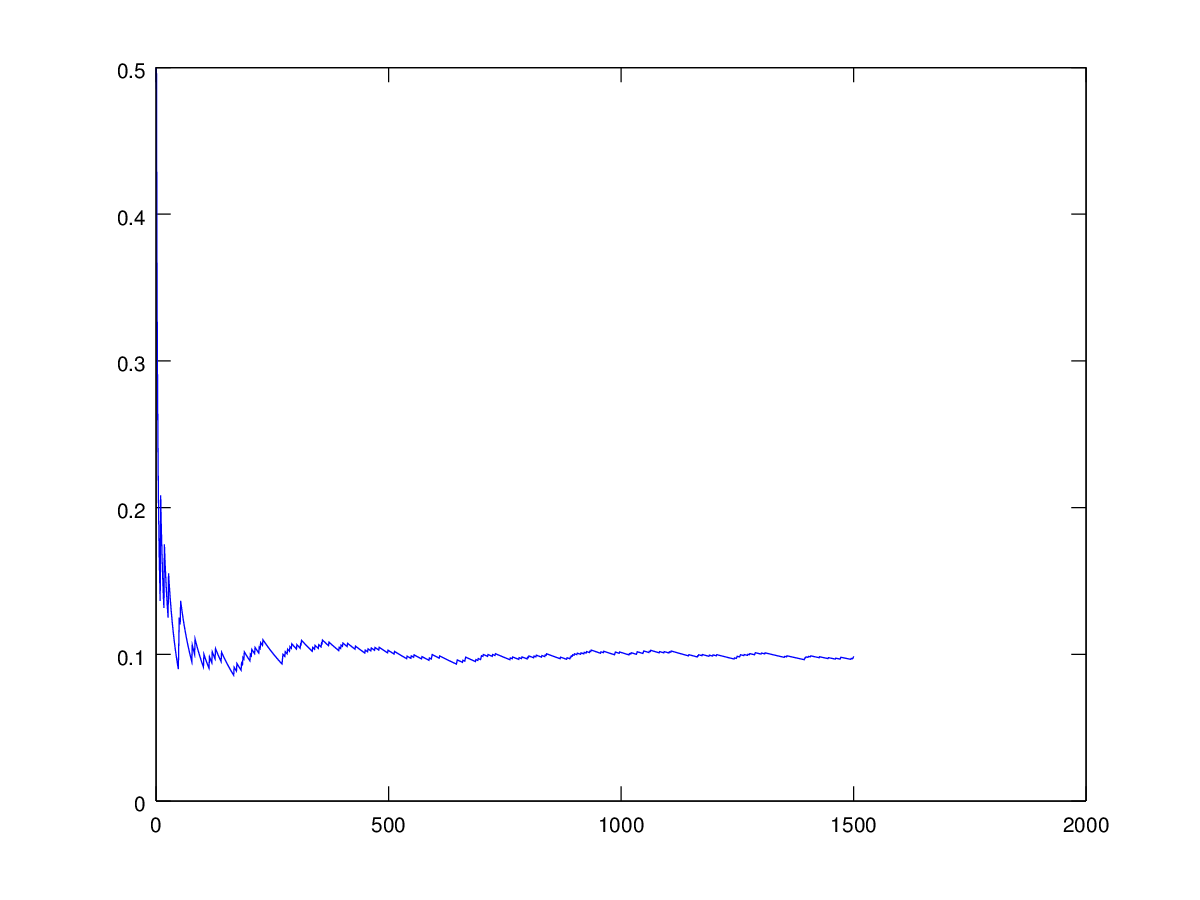
\includegraphics[width=0.7\textwidth]{poyla.png}
\caption{Urna de Poyla}
\label{Urna de Poyla}
\end{figure}


En esta gr\'afica se muestra la simulaci\'on de las urnas de Poyla. Como vimos en clase la proporci\'on de bolas rojas convergen, en esta gr\'afica se ilustra como la proporci\'on se tiende a estabilizar. Esto se debe al teorema de convergencia de martingalas ya que la martingala es positiva.

\end{ejercicio}

\begin{problema}[Ejercicios sueltos sobre martingalas]
\mbox{}\begin{enumerate}
\item Sea $\paren{X_n,n\geq 0}$ una sucesi\'on $\paren{\F_n}$-adaptada. Pruebe que\begin{esn}
\sum_{k=1}^n X_k-\espc{X_k}{\F_{k-1}}, \quad n\geq 0
\end{esn}es una $\paren{\F_n}$-martingala.

Demostraci\'on.

Denotemos a $M_n=\sum_{k=1}^n X_k-\espc{X_k}{\F_{k-1}}, \quad n\geq 0$.
\begin{enumerate}
\item Como $X_k$ es  $\F_k$-medible para todo $k\leq n$ entonces $X_k$ es $\F_n$-medible,ya que $X$ es $\F_n$-adaptada. Tambien sabemos por definici\'on de esperanza condicional que $\espc{X_k}{\F_{k-1}}$ es $\F_{k-1}$-medible, entonces $\espc{X_k}{\F_{k-1}}$ es $\F_n$-medible para todo $k\leq n$. Por lo tanto $M_n$ es $\F_n$-medible.
\item Por hip\'otesis $X_k\in L_1$ esto tambien nos indica que $\espc{X_k}{\F_{k-1}}\in L_1$, como $M_n$ es suma finita de variables aleatorias en $L_1$ entonces $M_n\in L_1$.

\item Propiedad de Martingala:
\begin{align}
\espc{M_n}{\F_{n-1}}&= \espc{\sum_{k=1}^n X_k-\espc{X_k}{\F_{k-1}}}{\F_{n-1}} \notag \\
&=\sum_{k=1}^n\espc{ X_k-\espc{X_k}{\F_{k-1}}}{\F_{n-1}} \notag \\
&=\sum_{k=1}^n\espc{ X_k}{\F_{n-1}}-\espc{\espc{X_k}{\F_{k-1}}}{\F_{n-1}} \notag
\intertext{Ya que $X_{k}$ es $\F_{n-1}$-medible para todo $k\leq n-1$}
&=\espc{ X_n}{\F_{n-1}}+\sum_{k=1}^{n-1} X_k-\sum_{k=1}^n\espc{\espc{X_k}{\F_{k-1}}}{\F_{n-1}} \notag
\intertext{Como $\espc{X_k}{\F_{k-1}}$ es $\F_{n-1}$-medible para toda $k\leq n$}
&=\espc{ X_n}{\F_{n-1}}+\sum_{k=1}^{n-1} X_k-\sum_{k=1}^n\espc{X_k}{\F_{k-1}} \notag \\
&=\sum_{k=1}^{n-1} X_k-\sum_{k=1}^{n-1}\espc{X_k}{\F_{k-1}} \notag \\
&=M_{n-1} \notag
\end{align}

Por lo tanto $M_n$ es martingala.
\end{enumerate}

\item{Descomposici\'on de Doob para submartingalas}: Sea Sea \(X=\paren{X_n}_{n\in\na}\) una submartingala. Pruebe que \(X\) se puede descomponer de manera \'unica como \(X=M+A\) donde \(M\) es una martingala y \(A\) es un proceso previsible con \(A_0=0\). Sugerencia: Asuma que ya tiene la descomposici\'on y calcule esperanza condicional de \(X_{n+1}\) dada \(X_n\). 

Como $X_n$ es submartingala podemos utilizar el inciso anterior para construir una martingala que dependa de $X_n$. A esa la denotaremos como $M_n=\sum_{k=1}^n X_k-\espc{X_k}{\F_{k-1}}+X_0$, al añadirle el $X_0$ sigue siendo martingala el proceso. Si suponemos que ya conocemos la descomposici\'on tenemos que:
\begin{esn}
X_n=M_n+A_n=\sum_{k=1}^n X_k-\espc{X_k}{\F_{k-1}}+X_0+A_n
\end{esn}
Despejando a $A_n$ tenemos que:
\begin{esn}
A_n=\sum_{k=1}^n \espc{X_k}{\F_{k-1}}-X_{k-1}
\end{esn}
Efectivamente $A_n$ es un proceso previsible ya que $\espc{X_k}{\F_{k-1}},X_{k-1}$ son $\F_{n-1}$-medibles.

Como $X_n$ es sub-martingala entonces $\espc{X_k}{\F_{k-1}\geq X_{k-1}}$. Por lo tanto $A_n$ es un proceso positivo. Por lo tanto las $A_n$ son crecientes.

La unicidad se da ya que si existen dos descomposiciones $M_n^1,A_n^1,M_n^2, A_n^2$ y si definimos $Y_n=M_n^1-M_n^2=A_n^1-A_n^2$. Por una parte tenemos que cumple la propiedad de Martingala y por otra parte cumple la propiedad de previsibilidad, es decir:
\begin{align}
\espc{Y_n}{\F_{n-1}}&=Y_{n-1} \notag \\
\espc{Y_n}{\F_{n-1}}&=Y_{n} \notag
\intertext{Si restamos las ecuaciones tenemos que:}
0&=Y_{n}-Y_{n-1} \notag \\
0&=A_{n}^{1}-A_{n-1}^{1}-(A_{n}^{2}-A_{n-1}^{2})\notag
\intertext{Como $A_{0}^{1}=0=A_{0}^{2}$ entonces tenemos que:}
0&=A_{1}^{1}-A_{1}^{2} \notag \\
A_{1}^{1}&=A_{1}^{2} \notag
\intertext{Recursivamente $A_{n}^{1}=A_{n}^{2}$ $\Rightarrow$ $Y=0$:}
M_{n}^{1}&=M_{n}^{2} \notag
\end{align}

Por lo tanto la descomposici\'on es \'unica.
\item Sea \(S_n=\xi_1+\cdots+\xi_n\) donde las variables \(\xi\) son independientes y \(\xi_i\) tiene media cero y varianza finita \(\sigma_i^2\). Pruebe que si \(\sum_i \sigma_i^2<\infty\) entonces \(S_n\) converge casi seguramente y en \(L_2\) conforme \(n\to\infty\). Construya un ejemplo de variables aleatorias \(\xi_i\) tales que la serie \(\sum_i \xi_i\) sea casi seguramente absolutamente divergente y casi seguramente condicionalmente convergente (considere ejemplos simples!). Explique heur\'isticamente por qu\'e cree que suceda esto.
%Ser\'a que \sum_i\abs{x_i}=\infty casi seguramente si \sum_i\abs\esp{\xi_i}=\infty? 

Sea $\F_n=\sag{\xi_1,\ldots,\xi_n}$. Hemos visto anteriormente que $\paren{X_n}_{n=1}^\infty$ es una martingala respecto a $\paren{\F_n}_{n=1}^\infty$. Adem\'as por la desigualdad de Cauchy-Schwartz, sabemos que\begin{esn}
\esp{\abs{X_n}}\leq \paren{\esp{X_n^2}}^{1/2}=\esp{\paren{\sum_{i=1}^n\xi_i}^2}^{1/2}
\end{esn}y como las variables aleatorias $\paren{\xi_i}_{i-1}^\infty$ son independientes y tienen media cero, su segundo momento es igual a su varianza  y la varianza de la suma (que corresponde tambi\'en  a su segundo momento) es igual a la suma de las varianzas, por lo que\begin{esn}
\esp{\abs{X_n}}\leq \paren{\sum_{i=1}^n\var{\xi_i}}^{1/2}\leq \paren{\sum_{i=1}^\infty\var{\xi_i}}^{1/2}<\infty,
\end{esn}por lo que la martingala $\paren{X_i}_{i=1}^\infty$ satisface las condiciones del teorema de convergencia casi segura de martingalas y por lo tanto, converge casi seguramente a una variable aleatoria que pertenece a $ L_1$.

El ejemplo es el siguiente:

Sea $\xi_i$ una variable aleatoria que toma los valores -1 y 1 con probabilidad $1/2$ Definimos la serie
$X_n=\sum_{i=1}^n \xi_i /i$, esta serie es casi seguramente absolutamente divergente debido a que.
\begin{esn}
\sum_{i=1}^{\infty} \abs{\xi_i}/i=\sum_{i=1}^{\infty} 1 /i=\infty .
\end{esn}



\item Sean \(X\) y \(Y\) dos martingalas (respecto de la misma filtraci\'on) y tales que \(\esp{X_i},\esp{Y_i}<\infty\) para toda \(i\). Pruebe la siguiente f\'ormula de integraci\'on por partes: $$ \esp{X_nY_n}-\esp{X_0Y_0}=\sum_{i=1}^n \esp{\paren{X_i-X_{i-1}}\paren{Y_i-Y_{i-1}}} . $$

Demostraci\'on

\begin{align}
\sum_{i=1}^n \esp{\paren{X_i-X_{i-1}}\paren{Y_i-Y_{i-1}}}&= \sum_{i=1}^n \esp{X_iY_i-X_{i-1}Y_i-X_iY_{i-1}+X_{i-1}Y_{i-1}} \notag \\
&=\sum_{i=1}^n \esp{X_iY_i}-\esp{X_{i-1}Y_i}-\esp{X_iY_{i-1}}+\esp{X_{i-1}Y_{i-1}} \notag \\
&=\sum_{i=1}^n \esp{X_iY_i}-\esp{\espc{X_{i-1}Y_i}{\F_{i-1}}} \notag \\
&-\esp{\espc{X_iY_{i-1}}{\F_{i-1}}}+\esp{X_{i-1}Y_{i-1}} \notag 
\intertext{Como $X_{i-1},Y_{i-1}$ son $F_{i-1}$-medibles:}
&=\sum_{i=1}^n \esp{X_iY_i}-\esp{X_{i-1}\espc{Y_i}{\F_{i-1}}} \notag \\
&-\esp{Y_{i-1}\espc{X_i}{\F_{i-1}}}+\esp{X_{i-1}Y_{i-1}} \notag 
\intertext{Como $X_i,Y_i$ son martingalas:}
&=\sum_{i=1}^n \esp{X_iY_i}-\esp{X_{i-1}Y_{i-1}} \notag \\
&-\esp{Y_{i-1}X_{i-1}}+\esp{X_{i-1}Y_{i-1}} \notag \\
&=\sum_{i=1}^n \esp{X_iY_i}-\esp{X_{i-1}Y_{i-1}} \notag \\
&=\esp{X_nY_n}-\esp{X_{0}Y_{0}}.
\end{align}

\item{Desigualdad de Azema-Hoeffding}
        \begin{enumerate}
        \item Muestre que si \(Y\) es una variable aleatoria con valores en \([-c,c]\) y media cero entonces, para \(\theta\in\re\)
                        $$\esp{e^{\theta Y}}\leq\imf{\cosh}{\theta c}\leq \imf{\exp}{\frac{1}{2}\theta^2c^2}. $$
                        
                        Como $e^{\theta y}$ es una funci\'on convexa tenemos que:
                        \begin{esn}
                        e^{\theta y}\leq \frac{c-y}{2c}e^{-\theta c}+\frac{c+y}{2c}e^{\theta c}=\frac{e^{\theta c}+e^{-\theta c}}{2}+y(\frac{e^{\theta c}-e^{-\theta c}}{2c})
                        \end{esn}
                        Calculando la esperanza de ambos lados de la desiguañdad obtenemos que:
                        \begin{esn}
                        \esp{e^{\theta Y}}\leq \esp{\frac{e^{\theta c}+e^{-\theta c}}{2}+Y\frac{e^{\theta c}-e^{-\theta c}}{2c}}
                        \end{esn}
                        Como la $\esp{Y}=0$, se sigue el resultado $\esp{e^{\theta Y}}\leq \cosh\paren{\theta c}$.
                        
                        Para la segunda parte de la desigualdad, nos fijamos en la expansion de Taylor de $\cosh\paren{\theta c}$:
                        \begin{align}
                      \cosh\paren{\theta c}&=\sum_{k=1}^\infty \frac{\paren{\theta c}^{2k}}{2k!} \notag \\
                      &\leq \sum_{k=1}^\infty \frac{\paren{\theta c}^{2k}}{2^k\paren{k!}} \notag \\
                      &=e^{\frac{\theta^2c^2}{2}}.\notag
                        \end{align} 
                        
        \item Pruebe que si \(M\) es una martingala nula en cero tal que para algunas constantes \(\paren{c_n,n\in\na}\) se tiene que
                        $$\abs{M_n-M_{n-1}}\leq c_n\quad\forall n $$
                        entonces, para \(x>0\)
                        $$
                        \proba{\max_{k\leq n} M_k\geq x}\leq \imf{\exp}{\frac{x^2}{2\sum_{k=1}^n c_k^2}}.
                        $$
                        En esta parte utilizaremos una  desigualdad de Doob que viene en las notas y dice que para una sub-martingala $M_n$ se tiene:
                        			\begin{esn} 
                        			\lambda\p\paren{\max_{1\leq i \leq n}M_i^+>\lambda} \leq \esp{M_n^+}
                        			\end{esn}
                        			En nuestro caso $M_n$ es martingala por lo que $e^{\theta M_n}$ es una sub-martingala positiva, aplicando la desigualdad de la proposici\'on anterior a esta sub-martingala  y tomando $\lambda = e^{\theta x}$ obtenemos que:
                        			\begin{esn}
                        			 e^{\theta x}\proba{\max_{1\leq i \leq n} e^{\theta M_i}> e^{ \theta x}} \leq \esp{ e^{\theta M_n}}
                        			\end{esn}
                        			Como $\set{\max_{1\leq i \leq n} e^{\theta M_i}> e^{\theta x}}=\set{\max_{1\leq i \leq n}  M_i>  x}$, entonces:
                        			\begin{esn}
                        			\proba{\max_{1\leq i \leq n}  M_i>  x} \leq  e^{-\theta x} \esp{ e^{\theta M_n}}
                        			\end{esn}
                        			Acotando a la martingala $M_n$ la cual es nula en $0$:
                        			\begin{align}
                        			\abs{M_n}&=\abs{\sum_{i=1}^{n}M_i-M_{i-1}}\notag \\
                        			&\leq \sum_{i=0}^{n}\abs{M_i-M_{i-1}}\notag \\
                        			&\leq\sum_{i=0}^{n}c_i=c^* \notag
                        			\end{align}
                        			Entonces $\abs{M_n}$ es acotada por $c^*$ por lo que podemos aplicar la desigualdad del ejercicio anterior
                        			\begin{esn}
                        			 \esp{ e^{\theta M_n}} \leq e^{\frac{1}{2}\theta^2(c^*)^2}
                        			\end{esn}
                        			Por lo tanto $\p\paren{\max_{1\leq i \leq n}  M_i>  x} \leq  e^{-\theta x} e^{\frac{1}{2}\theta^2(c^*)^2}$.Tomando a $\theta=\frac{x}{(c^*)^2}>0$, entonces
                        			\begin{align}
                        			\p\paren{\max_{1\leq i \leq n}  M_i>  x} &\leq exp\paren{-\frac{1}{2}\frac{x^2}{(c^*)^2}} \notag \\  &=exp\paren{\frac{-x^2}{2\paren{\sum_{i=1}^{n}c_i}^2}}\notag \\
                        			\end{align}
        \end{enumerate}
\end{enumerate}
\end{problema}
\begin{problema}
Sea $S_n=\sum_{i=1}^n X_i$ donde $X_1,X_2,\ldots$ son iid. Sea\begin{esn}
\imf{\phi}{\lambda}=\esp{e^{\lambda S_n}}\in (0,\infty].
\end{esn}
\begin{enumerate}
\item Pruebe que si existen $\lambda_1<0<\lambda_2$ tales que $\imf{\phi}{\lambda_i}<\infty$ entonces $\imf{\phi}{\lambda}<\infty$ para toda $\lambda\in [\lambda_1,\lambda_2]$. Sugerencia: escriba $\lambda=a\lambda_1+(1-a)\lambda_2$ para alg\'un $a\in [0,1]$ y aplique la desigualdad de H\"older. A partir de ahora se asume la premisa de este inciso.

Sea $\lambda\in [\lambda_1,\lambda_2]$ entonces $\exists$ $a\in [0,1]$ $\lambda=a\lambda_1+(1-a)\lambda_2$.

\begin{align}
\imf{\phi}{\lambda}&=\esp{e^{\lambda S_n}} \notag \\
&= \esp{e^{\paren{a\lambda_1+(1-a)\lambda_2} S_n}} \notag \\
&= \esp{e^{\paren{a\lambda_1}S_n}e^{(1-a)\lambda_2 S_n}} \notag
\intertext{Aplicando la desigualdad de Holder:}
&\leq \esp{e^{\paren{\lambda_1}S_n}}^a\esp{e^{\lambda_2 S_n}}^{1-a} \notag
\end{align}

Como la $\esp{e^{\paren{\lambda_1}S_n}}^a,\esp{e^{\lambda_2 S_n}}^{1-a}<\infty$ tenemos que $\imf{\phi}{\lambda}<\infty$ para toda $\lambda \in [\lambda_1,\lambda_2]$.

\item Pruebe que $\esp{\abs{S_n}^k}<\infty$ para toda $k\geq 0$. 

Sea $\lambda \in [\lambda_1,\lambda_2]$, definimos $X_m=\sum_{k=0}^{m}\frac{\abs{\lambda S_n}^k}{k!}$. Expresando como serie de taylor a $e^{\abs{\lambda S_n}}$ tenemos que:
\begin{align} 
\esp{e^{\abs{\lambda S_n}}}&=\esp{\lim_{m \rightarrow \infty}\sum_{k=0}^{m}\frac{\abs{\lambda S_n}^k}{k!}}\notag \\
&=\esp{\lim X_m}
\intertext{Como $X_m$ es una sucesi\'on creciente, ya que los terminos de la suma son positivos, se tiene  por el teorema de la convergencia mon\'otona que:}
&=\lim_{m \rightarrow \infty}\esp{X_m}\notag\\
&=\sum_{k=0}^{\infty}\frac{\abs{\lambda}^k \esp{\abs{S_n}^k}}{k!}\notag 
\end{align} 


Entonces:
\begin{align}
\esp{e^{\abs{\lambda S_n}}}&=\esp{e^{\lambda S_n}\indi{\lambda S_n \geq 0}}+\esp{e^{-\lambda S_n}\indi{\set{\lambda S_n <0}}} \notag \\
&\leq \esp{e^{\lambda S_n}}+\esp{e^{-\lambda S_n}} \notag
\intertext{Por inciso anterior tenemos que:}
&=\phi(\lambda)+\phi(-\lambda) < \infty. \notag
\end{align}


Por lo tanto $\sum_{k=0}^{\infty}\frac{\abs{\lambda}^k \esp{\abs{S_n}^k}}{k!}\ < \infty$.

Por lo tanto $\esp{\abs{S_n}^k} < \infty$ para toda $k\in \na$.

\item Sea $M^\lambda_t=e^{\lambda S_t}/\imf{\phi}{\lambda}$. Argumente que si $M^n$ es el proceso dado por\begin{esn}
M^n_t=\left.\frac{\partial^n}{\partial \lambda^n}\right|_{\lambda=0}M^\lambda_t,
\end{esn}entonces $M^n$ es una martingala para toda $n$.

Para demostrar esto primero mostraremos que el operador derivada sale de la esperanza condicional de una martingala  si la derivada de la martingala esta acotada. En general esto tambien sucede para el caso de variables aleatorias que no necesariamente son martingalas.

Si definimos $X_n=n\paren{M_t^{\lambda+\frac{1}{n}}-M_t^{\lambda}}$ y cuando $n \rightarrow \infty$ entonces $X_n$ converge a $\frac{\partial^1}{\partial \lambda^1}M^\lambda_t$. Por hip\'otesis tenemos que $\abs{\frac{\partial^1}{\partial \lambda^1}M^\lambda_t} < m(\omega)$ donde $m:\Omega \rightarrow R$ es integrable y notemos que:

\begin{align}
\abs{X_n}&=n\abs{\paren{M_t^{\lambda+\frac{1}{n}}-M_t^{\lambda}}}\notag \\ &=n\abs{\int_{\lambda}^{\lambda+\frac{1}{n}}\frac{\partial^1}{\partial \lambda^1}M^\lambda_t d\lambda} \notag \\ 
&\leq n\int_{\lambda}^{\lambda+\frac{1}{n}} \abs{\frac{\partial^1}{\partial \lambda^1}M^\lambda_t} d\lambda \notag \\
&\leq  n\int_{\lambda}^{\lambda+\frac{1}{n}} m(\omega) d\lambda \notag \\
&= m(\omega)n\paren{\lambda +\frac{1}{n}-\lambda}=m(\omega) \notag
\end{align} 

Por lo tanto $X_n$ es dominada por $m(\omega)$.

Ahora aplicando el teorema de convergencia dominada para la integral 

\begin{align}
\espc{\frac{\partial^1}{\partial \lambda^1}M^\lambda_t}{\G}&=\espc{\lim_{n \rightarrow \infty}X_n}{\G} \notag \\
&=\lim_{n \rightarrow \infty}\espc{X_n}{\G}\notag \\
&=\lim_{n \rightarrow \infty}\espc{n\paren{M_t^{\lambda+\frac{1}{n}}-M_t^{\lambda}}}{\G} \notag \\
&=\lim_{n \rightarrow \infty}n\paren{\espc{M_t^{\lambda+\frac{1}{n}}}{\G}- \espc{M_t^{\lambda}}{\G}  }\notag \\ &=\frac{\partial^1}{\partial \lambda^1}\espc{M^\lambda_t}{\G} \notag
\end{align}

Ya demostrado esto procederemos a probar la propiedad de martingala por induccion sobre $n$. Para el caso $n=1$, sabemos que $M_t^\lambda$ es martingala por ejercicio 5 de la tarea. Entonces, suponiendo que existe una variablea leatoria $Y$ tal que $\abs{\frac{\partial^1}{\partial \lambda^1}M^\lambda_t}<Y$:

\begin{align}
\espc{\frac{\partial^1}{\partial \lambda^1}M^\lambda_t}{\F_{t-1}}&=\frac{\partial^1}{\partial \lambda^1}\espc{M^\lambda_t}{\F_{t-1}} \notag \\
\notag =\frac{\partial^1}{\partial \lambda^1}M^{\lambda}_{t-1} \notag
\end{align}

Suponiendo que el caso $n=k$ es martingala. Demostraremos caso $n=k+1$:
\begin{align}
\espc{\frac{\partial^{k+1}}{\partial \lambda^{k+1}}M^\lambda_t}{\F_{t-1}}&=\frac{\partial^1}{\partial \lambda^1}\espc{\frac{\partial^{k}}{\partial \lambda^{k}}M^\lambda_t}{\F_{t-1}} \notag
\intertext{Utilizando hipotesis de inducci\'on:}
&=\frac{\partial^1}{\partial \lambda^1}\frac{\partial^{k}}{\partial \lambda^{k}}M^\lambda_{t-1}\notag \\
&=\frac{\partial^{k+1}}{\partial \lambda^{k+1}}M^\lambda_{t-1}.\notag
\end{align}

Por lo tanto $\frac{\partial^{k+1}}{\partial \lambda^{k+1}}M^\lambda_t$ es martingala.

Por lo tanto $\frac{\partial^{n}}{\partial \lambda^{n}}M^\lambda_t$ es martingala para toda $n\in \na$.

En particular si se eval\'ua en $\lambda =0$ se obtiene el resultado.

\item Calcule las primeras $4$ martingalas resultantes si $\proba{X_i=\pm 1}=1/2$. Util\'icelas para calcular el valor de $\esp{T^2}$ donde\begin{esn}
T=\min\set{n\geq 0: S_n\in\set{-a,a}}
\end{esn}y $a>0$.

Si derivamos y evaluamos en $\lambda=0$, obtenemos que:
\begin{esn}
\left.\frac{\partial^{(k)}}{\partial \lambda^{k}}\right|_{\lambda=0} \phi(\lambda) =\left.\esp{\frac{\partial^{(k)}}{\partial \lambda^{k}} \right|_{\lambda=0}e^{\lambda S_n}} =\esp{S_n^k} < \infty
\end{esn}

Esto nos \'indica que podemos obtener los momentos de $S_n$. Como estamos en una caminata aleatoria obtenemos que:
\begin{align}
\esp{S_n}&=0= \left.\frac{\partial^{(1)}}{\partial\lambda^{1}} \right|_{\lambda=0}\phi(\lambda) \notag \\ \esp{S_n^2}&=n=\left.\frac{\partial^{(2)}}{\partial \lambda^{2}}\right|_{\lambda=0}\phi(\lambda) \notag \\ \esp{S_n^3}&=0=\left.\frac{\partial^{(3)}}{\partial \lambda^{3}}\right|_{\lambda=0} \phi(\lambda) \notag \\ \esp{S_n^4}&=3n^2-2n=\left.\frac{\partial^{(4)}}{\partial \lambda^{4}}\right|_{\lambda=0} \phi(\lambda)\notag
\end{align}
De aqui obtenemos las martingalas:
\begin{align}
M^1_t&=\left.\frac{\partial^1}{\partial \lambda^1}\right|_{\lambda=0}M^\lambda_t=S_t \notag \\ M^2_t&=\left.\frac{\partial^2}{\partial \lambda^2}\right|_{\lambda=0}M^\lambda_t=S_t^2-t \notag \\ M^3_t&=\left.\frac{\partial^3}{\partial \lambda^3}\right|_{\lambda=0}M^\lambda_t=S_t^3-3tS_t \notag \\
M^4_t&=\left.\frac{\partial^4}{\partial \lambda^4}\right|_{\lambda=0}M^\lambda_t=S_t^4-6tS_t^2+3t^2+2t \notag
\end{align}

Luego entonces podemos $S_T$  es una variable que toma un valor ya que $a=b$:
\begin{align}
\proba{S_T=-a}&=\frac{a}{2a} \notag \\
\proba{S_T=a}&=\frac{a}{2a} \notag
\end{align}
Entonces: 
\begin{align}
\esp{S_T}&=0 \notag \\
\esp{S_T^2}&=a^2 \notag \\
\esp{S_T^3}&=0 \notag \\
\esp{S_T^4}&=\frac{a^2(2a^3)}{2a}. \notag
\end{align}
Por el muestro opcional de Doob y como las martingalas obtenidas tiene media cero:
\begin{align}
0&=\esp{S_T^4-6TS_T^2+3T^2+2T}=\esp{S_T^4}-6\esp{TS_T^2}+3\esp{T^2}+2\esp{T}\notag \\
\Rightarrow\esp{T^2}&=\frac{6\esp{TS_T^2}-\frac{a^2(2a^3)}{2a}-2a^2}{3} \notag
\end{align}
Ya que $a=b$ entonces $S_T^2$ solo toma una valor que es $a^2$:
\begin {esn}
\esp{T^2}=\frac{6\esp{Ta^2}-\frac{a^2(2a^3)}{2a}-2a^2}{3}=\frac{a^2(5a^2-2)}{3}
\end{esn}
 

\end{enumerate}

\defin{Categor\'ias:} Caminatas aleatorias, muestreo opcional, ejemplos de martingalas. 
\end{problema}

\begin{problema}
Sea $M$ una $\paren{\F_n}$-martingala. Pruebe que si $T$ es un tiempo de paro finito entonces $\esp{M_T}=\esp{M_0}$ bajo cada una de las siguientes condiciones:
\begin{enumerate}
\item $M$ es acotada.

Si $M$ es acotada entonces $\abs{M_n}\leq K$ para toda $n\in\na$ esto implica que $M_{T\wedge n}$ tambien es acotada. Adem\'as como $T\wedge n$ es un tiempo de paro acotado por el teorema de muestreo opcional de Doob entonces $\esp{M_{T\wedge n}}=\esp{M_0}$. Ya que $M_{T\wedge n}$ converge a $M_T$, aplicande el teorema de convergencia acotada tenemos que $\esp{M_{T\wedge n}}$ converge a $\esp{M_{T}}$ pero la esperanza de $\esp{M_{T\wedge n}}=\esp{M_{0}}$ para toda $n\in \na$. Por lo tanto $\esp{M_T}=\esp{M_0}$.


\item $T$ es integrable y la sucesi\'on $\paren{M_n-M_{n-1}}$ es acotada.

Como la sucesi\'on $\paren{M_n-M_{n-1}}$ es acotada entonces $\abs{\paren{M_n-M_{n-1}}}\leq K$.
\begin{esn}
\abs{\paren{M_{T\wedge n}-M_{0}}}=\abs{\sum_{i=1}^{T\wedge n}\paren{M_i-M_{i-1}}}\leq\sum_{i=1}^{T\wedge n}\abs{\paren{M_i-M_{i-1}}}\leq T K.
\end{esn}

Entonces la sucesi\'on $M_{T\wedge n}-M_{0}$ dominada por $KT$. Utilizando el teorema de muestreo opcinal de Doob sabemos que $\esp{M_{T\wedge n}-M_{0}}=0$ para toda $n\in \na$. Podemos utiliar el teorema e convergencia dominada ya que $KT$ es integrable entonces $\esp{M_T-M_0}=0$. Por lo tanto $\esp{M_T}=\esp{M_0}$.
\item $\paren{M_{n\wedge T}}$ es uniformemente integrable.

Sabemos que $M_{n\wedge T}$ converge a $M_T$,  ademas como $M_{n\wedge T}$ es uniformemente integrable sabemos que $M_{T}$ es integrable y $\esp{M_{n\wedge T}}$ converge a $\esp{M_{T}}$. Pero por el teorema de muestreo opcional de Doob como $T\wedge n$ es un tiempo de paro acotado la $\esp{M_{T\wedge n}}=\esp{M_0}$. Por lo tanto $\esp{M_{T}}=\esp{M_0}$.

\end{enumerate}

\defin{Categor\'ias: } Muestreo opcional. 
\end{problema}

\begin{problema}
Sea $M$ una $\paren{\F_n}$-martingala con saltos acotados. Sean
\begin{esn}
C=\set{\limsup M_n=\liminf M_n\in\re}\quad\text{y}.
\end{esn}
Pruebe que $\proba{C\cup D}=1$. Deduzca que las caminatas aleatorias centradas con saltos acotados oscilan. Sugerencia: Para cada $K>0$ defina\begin{esn}
T=\min\set{n\geq 0: \abs{M_n}\geq K}
\end{esn}y aplique el teorema de convergencia de martingalas a $M^T$. 

Sea $M$ una caminata aleatoria no trivial con saltos integrables en $-1,0,1,\ldots$ y  media cero. Pruebe que $\proba{M\text{ converge en }\na}=0$ y  concluya que $\liminf M_n=-\infty$ casi seguramente. (Este resultado permitir\'a dar una prueba adicional de que un Galton-Watson cr\'itico se extingue).  Sugerencia: proceda como en el p\'arrafo anterior y pruebe la integrabilidad uniforme de $M_{T\wedge n},n\in\na$.

\defin{Categor\'ias: } Teoremas de convergencia de martingalas

Sea:
\begin{esn}
T_q=\min{\set{n>0: M_n\leq -q}}\textrm{ $q \in \mathbb{Q}$}
\end{esn}

$T_q$ es un tiempo de paro ya que:
\begin{esn}
\set{T_q=n}=\set{M_i\geq -q \text{ para todo $i\in\set{1,2,3,..,n-1}$}, M_n\leq -q}
\end{esn}
como $M_n$ es martingala entonces $\set{T_q=n}\in \F_n$.


Por hip\'otesis tenemos que  $\abs{M_i-M_{i-1}} < C$ para alg\'un $C>0$, de aqui obtenemos que $
M_{T_q\wedge n}\geq -q-C$   $\Rightarrow M_{T_q\wedge n} + q + C \geq  0 \textrm{ para toda n}$. Por ser
$M_{T_q\wedge n} $  martingala, entonces $M_{T_q\wedge n} + q + C$ es una martingala positiva. Por lo tanto $M_{T_q\wedge n}+q+C$   converge. Por lo tanto $M_{T_q\wedge n}$ converge. En el  conjunto  $\set{T_q=\infty}$ se tiene que $M_n$ converge. Si nos fijamos en el conjunto $\set{\liminf_n{M_n}>-\infty}$ tambi\'en $M_n$ converge ya que:
\begin{esn}
\bigcup_q\set{T_q=\infty}=\set{\liminf_n{M_n}>-\infty}.
\end{esn}
Utilizando el mismo argumento para el tiempo de paro $T_q=\min{\set{n>0: M_n \geq q}}$ obtenemos que en el conjunto $\limsup_n{M_n}=\infty$ $M_n$ converge. Por lo tanto $\proba{C\bigcup D}=1$.

Si tomamos una caminata aleatoria $S_n=\sum_{i=1}^{n}\xi_i$  con saltos acotados tenemos que:

\begin{align} 
&\proba{S_N=k,S_{N+1}=k,S_{N+2}=k,...,S_{N+n}=k} \notag \\
&=\proba{S_N=k}\proba{\xi_{N+1}=0,\xi_{N+2}=0,...,\xi_{N+n}=0}\notag \\
&=\proba{S_N=k}\proba{\xi_{1}=0}^n. \notag
\end{align}

Como es una caminata aleatoria no trivial $\proba{\xi_{1}=0}^n>0$ entonces Cuando $n\rightarrow\infty $ entonces notamos que $S_n$ no converge. Por lo tanto las caminatas aleatorias con saltos acotados oscilan.

Si tenemos una martingala que tienes saltos integrables y definimos el tempo de paro $T_q=\min \set{n>0 : \abs{M_n}>q}$, entonces tenemos que $\abs{M_{T_q\wedge n}}<\xi_{T_q\wedge n}+q$.De aqui:

\begin{align}
\abs{M_{T_q\wedge n}}\indi{M_{T_q\wedge n}>c}&<\paren{\xi_{T_q\wedge n}+q}\indi{\xi_{T_q\wedge n}>c}\notag \\
\Rightarrow\sup_n\esp{\abs{M_{T_q\wedge n}}\indi{M_{T_q\wedge n}>c}}&<\sup_n\esp{ \paren{\xi_{T_q\wedge n}+q}\indi{\xi_{T_q\wedge n}>c}}\notag \\
\Rightarrow\lim_{c\rightarrow \infty}\sup_n\esp{\abs{M_{T_q\wedge n}}\indi{M_{T_q\wedge n}>c}}&< \lim_{c\rightarrow \infty} \sup_n \esp{\paren{\xi_{T\wedge n}+q}\indi{\xi_{T_q\wedge n}>c}} \notag \\
&=\lim_{c\rightarrow \infty} q \proba{\xi_1 >c }+\esp{\xi_{1}\indi{\xi_{1}>c}}=0 \notag
\end{align}

Por lo tanto $M_{T_q\wedge n}$ es uniformemente integrable. Por lo tanto la martingala $M_{T_q\wedge n}$ converge.

Haciendo el mismo razonamiento que en el caso de saltos acotados tenemos que la martingala $M_n$ converge en el conjunto $\set{T_q=\infty}$. En caso contrario la martingala diverge.

Por lo tanto en el caso de martingalas con saltos integrables $\proba{C\bigcup D}=1$.

Por el mismo argumento que en el caso de las caminatas aleatorias con saltos acotados las caminatas aleatorias con satos integrables oscilan. Por lo tanto el $\liminf M_n=-\infty$ casi seguramente.

\end{problema}



\begin{problema}
Sean $X_1,X_2,\ldots$ variables aleatorias intercambiables:\begin{esn}
\paren{X_1,\ldots, X_n}\stackrel{d}{=}\paren{X_{\pi_1},\ldots, X_{\pi_n}}
\end{esn}para cada permutaci\'on $\sigma$ de $\set{1,\ldots,n}$. 
\begin{enumerate}
\item Para $\G,\h$ sub$\sigma$-\'algebras de $\F$ definimos a $\G\vee\h=\sag{\G\cup\h}$. Sea \begin{esn}
\G^n=\sag{\imf{f}{X_1,\ldots, X_n}: \fun{f}{\re^n}{\re}\text{ es sim\'etrica}}\vee\sag{X_{n+1},X_{n+2},\ldots}. 
\end{esn}Pruebe que $\G^n,n\geq 1$ es una filtraci\'on al rev\'es. Sea $\G$ su intersecci\'on.
\item Para cada $A\in\mc{B}_{\re}$, defina a\begin{esn}
\imf{\Xi_n}{A}=\frac{1}{n}\sum_{i=1}^n \indi{X_i\in A}.
\end{esn}Pruebe que\begin{esn}
\probac{X_1\in A}{\G^n}=\imf{\Xi_n}{A}. 
\end{esn}?`Por qu\'e puede definir a  $\imf{\Xi}{A}=\lim_{n\to\infty}\imf{\Xi_n}{A}$?


Si definimos las variables, $Y_1=\indi{\set{X_1 \in A}}$, $Y_2=\indi{\set{X_2 \in A}}$, ..., 
entonces $Y_i \in \set{0,1}$ y adem\'as  son intercambiables ya que:
\begin{align}
\proba{Y_1=i_1,... ,Y_n=i_n}&=\proba{\indi{X_1 \in A}=i_1,... , \indi{X_n \in A}=i_n} \notag \\
&=\proba{\indi{X_{\pi(1)} \in A}=i_1,... , \indi{X_{\pi(n)} \in A}=i_n} \notag \\
&= \proba{Y_{\pi(1)}=i_1,... ,Y_{\pi(n)}=i_n} \notag
\end{align}
Por teorema visto en clase sabemos que para cual quier funci\'on $h$ medible:
\begin{esn}
\espc{h(Y_1,...,Y_n)}{\G_n}=\espc{h(Y_{\pi(1)},...,Y_{\pi(n)})}{\G_n}
\end{esn}
Entonces si tomamos $h$ como $h(Y_1,\ldots,Y_n)=Y_1$ tenemos que:
\begin{esn}
\espc{Y_j}{\G_n}=\espc{Y_1}{\G_n}
\end{esn}
para toda $j \leq n$
Si definimos la funci\'on $f(Y_1,...,Y_n)=\frac{1}{n}\sum_{i=1}^{n}Y_i$ es sim\'etrica entonces $\frac{1}{n}\sum_{i=1}^{n}Y_i$ es $\G^n$-medible y adem\'as:
\begin{esn}
 \frac{1}{n}\sum_{i=1}^{n}Y_i=\espc{\frac{1}{n}\sum_{i=1}^{n}Y_i}{\G^n}=\frac{1}{n}\sum_{i=1}^{n}\espc{Y_i}{\G^n}=\espc{Y_1}{\G^n}
\end{esn}
Por lo tanto:
\begin{esn}
\imf{\Xi_n}{A}:= \frac{1}{n}\sum_{i=1}^{n}\indi{X_i\in A}=\espc{\indi{X_1 \in A}}{\G^n}=\p(X_1 \in A| \G^n)
\end{esn}
Ahora definamos:
\begin{esn}
M_n=\espc{Y_1}{\G^n}=\frac{1}{n}\sum_{i=1}^{n}\indi{X_i\in A},
\end{esn}
y demostremos que es martingala reversa:
\begin{enumerate}
\item Por construcci\'on $M_n$ es $\G_n$-medible
\item $M_n$ es integrable ya que:
\begin{esn}
\esp{\abs{M_n}}=\esp{\abs{\espc{Y_1}{\G^n}}}\leq \esp{\espc{\abs{Y_1}}{\G^n}} =\esp{\abs{Y_1}}<\infty
\end{esn}
Por lo tanto $M_n$ es integrable.
\item Propiedad de martingala reversa:
\begin{align}
\espc{M_n}{\G^{n+1}}&=\espc{\frac{1}{n}\sum_{i=1}^{n}\indi{X_i\in A}}{\G^{n+1}}\notag \\ 
&=\frac{1}{n}\sum_{i=1}^{n}\espc{Y_i}{\G^{n+1}}\notag \\
&=\espc{Y_1}{\G^{n+1}}\notag \\
&=M_{n+1} \notag
\end{align}
\end{enumerate}

Por lo tanto $M_n$ es martingala reversa. Por teorema visto en clase $M_n$ es uniformemente integrable y por tanto  converge casi seguramente y en $L_1$.
Por lo tanto podemos definir $\imf{\Xi}{A}=\lim_{n\to\infty}\imf{\Xi_n}{A}$

\item Al considerar a la martingala\begin{esn}
\frac{1}{n\paren{n-1}}\sum_{1\leq i<j\leq n}\indi{X_i\in A}\indi{X_j\in A},
\end{esn}pruebe que $\probac{X_1\in A,X_2\in A}{\G}=\probac{X_1\in A}{\G}\probac{X_2\in A}{\G}$. Extienda la afirmaci\'on de independencia condicional anterior a $X_1,\ldots, X_n$.

Por inciso anterior sabemos que:
\begin{esn}
\probac{X_1 \in A}{\G}=\espc{\indi{X_1 \in A}}{\G}=\espc{Y_1}{\G}=\lim_{n \rightarrow \infty}\frac{1}{n}\sum_{i=1}^{n}{\indi{X_i \in A}}
\end{esn}
Ahora si tomamos $h(Y_1,...,Y_n)=Y_2$ obtenemos que:
\begin{esn}
\probac{X_2 \in A}{\G}=\espc{\indi{X_2 \in A}}{\G}=\espc{Y_2}{\G}=\lim_{n \rightarrow \infty}\frac{1}{n}\sum_{i=1}^{n}{\indi{X_i \in A}}
\end{esn}
Ahora notemos que $f(Y_1,\ldots,Y_n)=\frac{1}{n\paren{n-1}}\sum_{1\leq i \neq j\leq n}Y_iY_j$ es sim\'etrica entonces $\frac{1}{n\paren{n-1}}\sum_{1\leq i \neq j\leq n}Y_iY_j$ es $\G^n$-medible. Entonces:
\begin{align}
\frac{1}{n\paren{n-1}}\sum_{1\leq i \neq j\leq n}Y_iY_j&=\espc{\frac{1}{n\paren{n-1}}\sum_{1\leq i \neq j\leq n}Y_iY_j}{\G^n} \notag \\
&=\espc{Y_1Y_2}{\G^n} \notag
\end{align}
sPor lo tanto $M_n=\frac{1}{n\paren{n-1}}\sum_{1\leq i \neq j\leq n}Y_iY_j $ es martingala reversa entonces converge casi seguramente y en $L_1$. $M_n$ converge a $M_\infty=\espc{Y_1Y_2}{\G^\infty}=\espc{Y_1Y_2}{\G}$. De aqui obtenemos que:
\begin{align}
\probac{X_1 \in A, X_2 \in A}{\G}&=\espc{Y_1Y_2}{\G}\notag \\
&=\lim_{n \rightarrow \infty}\frac{1}{n\paren{n-1}}\sum_{1\leq i \neq j\leq n}Y_iY_j \notag \\
&=\lim_{n \rightarrow \infty}\frac{1}{n\paren{n-1}}( \paren{\sum_{i=1}^{n}{Y_i}}\paren{\sum_{j=1}^{n}{Y_j}} -\sum_{i=1}^{n}Y_i^2) \notag
\intertext{Ya que $Y_i^2=\paren{\indi{X_i \in A}}^2=\indi{X_i \in A}=Y_i$:}
&=\lim_{n \rightarrow \infty}\frac{1}{n\paren{n-1}}(\paren{\sum_{i=1}^{n}{Y_i}}\paren{\sum_{j=1}^{n}{Y_j}-1})\notag \\
&=\lim_{n \rightarrow \infty}\frac{\sum_{i=1}^{n}{Y_i}}{n}\paren{\frac{ \sum_{i=1}^{n}{Y_i}}{n-1}-\frac{1}{n-1}}\notag \\
&=\lim_{n \rightarrow \infty}\paren{\frac{\sum_{i=1}^{n}{Y_i}}{n}}\paren {\paren{ \frac{ \sum_{i=1}^{n}{Y_i}}{n}} \paren{ \frac{n}{n-1}}-\frac{1}{n-1}}\notag \\
&=\paren{\lim_{n \rightarrow \infty}\frac{\sum_{i=1}^{n}{Y_i}}{n}}\paren{\paren{\lim_{n \rightarrow \infty}\frac{\sum_{i=1}^{n}{Y_i}}{n}}\paren{\lim_{n \rightarrow \infty}\frac{n}{n-1}}-\paren{\lim_{n \rightarrow \infty}\frac{1}{n-1}}}\notag \\
&=\paren{\lim_{n \rightarrow \infty}\frac{\sum_{i=1}^{n}{Y_i}}{n}}\paren{\lim_{n \rightarrow \infty}\frac{\sum_{i=1}^{n}{Y_i}}{n}}\notag \\
&=\probac{X_1 \in A}{\G}\probac{X_2 \in A}{\G} \notag
\end{align}

Por lo tanto:
\begin{esn}
\probac{X_1\in A,X_2\in A}{\G}=\probac{X_1\in A}{\G}\probac{X_2\in A}{\G}
\end{esn}


\end{enumerate}

\defin{Cagegor\'ias: }Teorema de convergencia de martingalas, teorema de de Finetti.
\end{problema}

\begin{ejercicio}
\mbox{}
\begin{enumerate}
\item Ejecute y explique la funci\'on del siguiente c\'odigo en Octave. Comente qu\'e teoremas del curso (y del curso de probabilidad) son importantes para interpretar la figura.

\item Ejecute y explique la funci\'on del siguiente c\'odigo en Octave. Incluya una gr\'afica en la que la longitud de la variable k sea mayor a 1000. (Puede modificar el programa...) En la gr\'afica observara un esbozo de la trayectoria de un proceso de ramificaci\'on continuo (en una escala distinta...).


\end{enumerate}
\end{ejercicio}

\begin{problema}
Sean $\F_1,\F_2,\ldots $ y $\G$ sub\sa s de $\F$. Decimos que $\F_1,\F_2,\ldots$ son condicionalmente independientes dada $\G$ si para cualquier $H_i$ que sea $\F_i$ medible y acotada se tiene que\begin{esn}
\espc{H_1\cdots H_n}{\G}=\espc{H_1}{\G}\cdots \espc{H_n}{\G}.
\end{esn}
\begin{enumerate}
\item ?`Qu\'e quiere decir la independencia condicional cuando $\G=\set{\oo,\emptyset}$?
\begin{proof}

Si $\G=\set{\oo,\emptyset}$ entonces $\espc{X}{\G}=\esp{X}$. Pir lo tanto la defininci\'on de de independecia condicional se convierte en la propiedad de independencia:
\begin{esn}
\esp{H_1...H_n}=\esp{H_1}...\esp{H_n}.
\end{esn}

\end{proof}

\item Pruebe que $F_1$ y $\F_2$ son condicionalmente independientes dada $\G$ (denotado $\condind{\F_1}{\F_2}{\G}$) si y s\'olo si para cualquier $H$ que sea $\F_1$-medible y acotada se tiene que\begin{esn}
\espc{H}{\F_2,\G}=\espc{H}{\G}.
\end{esn}

Primero supondremos $F_1$ y $\F_2$ son condicionalmente independientes dada $\G$. La demostraci\'on la haremos utilizando el lema de clases mon\'otonas. Definiremos a nuestro $\pi$-sistema $C=\set{A\bigcap B: A\in \G B\in \F_2}$, evientemente es $\pi$-sistema, nuestro $\lambda$-sistema $L=\set{A\in\sigma(F_2\bigcup\G):\esp{H\indi{A}}=\esp{\espc{H}{\G}\indi{A} } } $ donde $H$ es $\F_1$-medible. Primero demonstraremos que $C\subseteq L$, sea $A\bigcap B\in C$:

\begin{align}
\esp{H\indi{A\bigcap B}} &=\esp{H\indi{A}\indi{ B}}\notag \\
&=\esp{\espc{H\indi{A}\indi{ B}}{\G}}\notag \\
&=\esp{\indi{A}\espc{H\indi{ B}}{\G}} \notag \\
&=\esp{\indi{A}\espc{H}{\G}\espc{\indi{ B}}{\G}}\notag \\
&=\esp{\espc{\indi{A}\espc{H}{\G}\indi{ B}}{\G}}\notag \\
&=\esp{\espc{H}{\G}\indi{A}\indi{ B}}\notag
\end{align}

Por lo tanto $C\subseteq L$.

Ahora mostrartemos que $L$ es $\lambda$-sistema. Sea $(A_i)\in L$ creciente, entonces:
\begin{align}
\esp{H\indi{\bigcup_{i\in \na} A_i}} &= \lim_{n\rightarrow\infty}\esp{H\indi{A_n}} \notag \\
&=  \lim_{n\rightarrow\infty}\esp{\espc{H}{\G}\indi{A_n}} \notag \\
&= \esp{\espc{H}{\G}\indi{\bigcup_{n\in \na} A_n}} \notag 
\end{align}

Por lo tanto $\bigcup_{n\in \na} A_n\in L$.

Sea $A,B\in \na$ $A\subseteq B$, entonces:

\begin{align}
\esp{H\indi{B-A}} &=\esp{H (\indi{B}-\indi{A})} \notag \\
&=\esp{H \indi{B}}-\esp{H\indi{A}} \notag \\
&=\esp{\espc{H}{\G}\indi{B}}-\esp{\espc{H}{\G}\indi{A}}   \notag \\
&=\esp{\espc{H}{\G}\indi{B-A} } \notag 
\end{align}

Por lo tanto $B-A\in L$.

Por lo tanto $L$ es $\lambda$-sistema.

Utilizando el teorema de clases mon\'otonas se obtiene el resultado.

Ahora supondremos que para cualquier $H$ que sea $\F_1$-medible y acotada se tiene que
\begin{esn}
\espc{H}{\F_2,\G}=\espc{H}{\G}.
\end{esn}

Sea $A\in \G$ entonces:

\begin{align}
\esp{H_1H_2\indi{A}}&=\esp{\espc{H_1H_2\indi{A}}{\sigma \paren{\F_2\bigcup \G}}}\notag \\
&=\esp{H_2\indi{A}\espc{H_1}{\sigma \paren{\F_2\bigcup \G}}}\notag \\
&=\esp{H_2\indi{A}\espc{H_1}{\G}}\notag \\
&=\esp{\espc{H_2\indi{A}\espc{H_1}{\G}}{\G}}\notag \\
&=\esp{\indi{A}\espc{H_1}{\G}\espc{H_2}{\G}}\notag
\end{align}

Por lo tanto $F_1$ y $F_2$ son condicionalmente independientes dado $\G$.


\item Pruebe que $\F_1,\F_2,\ldots, $ son condicionalmente independientes dada $\G$ si y s\'olo si para cada $n\geq 1$, $\F_{n+1}$ es condicionalmente independiente de $\F_1,\ldots, \F_n$ dada $\G$.

\begin{proof}

Supongamos que $\F_1,\F_2,\ldots, $ son condicionalmente independientes dada $\G$. Utilizando el ejercicio anterior basta probar que para $H_{n+1}$ que sea $\F_{n+1}$ medible y acotada entonces:
\begin{esn}
\espc{H_{n+1}}{\sigma\paren{\F_1\cup...\cup\F_n\cup\G}}=\espc{H_{n+1}}{\G}
\end{esn}

Lo demostraremos utilizando el lema de clases mon\'otonas. Sea $\C=\set{A\in\sigma\paren{\F_1\cup...\cup\F_n\cup\G}: A=\bigcap_{i=1}^{n}\bigcap G, A_i\in\F_i,G\in\G}$, claramente es un $\pi$-sistema, y sea $L=\set{A\in\sigma\paren{\F_1\cup...\cup\F_n\cup\G}:\esp{H_{n+1}\indi{A}}=\esp{\espc{H_{n+1}}{\G}}\indi{A}} $, para checar que es $\lambda$-sistema se hace una prueba similar al inciso anterior. Solo nos falta probar que $\C \subseteq L$, sea $C\in \C$:

\begin{align}
\esp{H_{n+1}\indi{C}}&=\esp{H_{n+1}\indi{A_1}\indi{A_2}...\indi{A_n}\indi{G}} \notag \\
&=\esp{\indi{G} \espc{H_{n+1}\indi{A_1}\indi{A_2}...\indi{A_n}}{\G}}\notag
\intertext{Como $\F_1,\F_2,\ldots, $ son condicionalmente independientes dada $\G$:}
&=\esp{\indi{G}\espc{H_{n+1}}{\G} \espc{\indi{A_1}\indi{A_2}...\indi{A_n}}{\G}}\notag \\
&=\esp{ \espc{\indi{G}\espc{H_{n+1}}{\G}\indi{A_1}\indi{A_2}...\indi{A_n}}{\G}}\notag \\
&=\esp{\espc{\espc{H_{n+1}}{\G}\indi{C}}{\G}} \notag \\
&=\esp{\espc{H_{n+1}}{\G}\indi{C}} \notag
\end{align}

Por lo tanto $\C \subseteq L$.Utilizando el lema de clases mon\'otonas se obtiene el resultado para cualquier $A\in\sigma\paren{\F_1\cup...\cup\F_n\cup\G}$.

Ahora supondremos que para cada $n\geq 1$, $\F_{n+1}$ es condicionalmente independiente de $\F_1,\ldots, \F_n$ dada $\G$. La demostraci\'on se har\'a por inducci\'on, para el caso $n=1$ se cumple, ya que por la hip\'otesis sabemos que $\F_2$ es condicionalmente independiente de $\F_1$ dado $\G$. Ahora supongamos que $\F_1,...,\F_n$ son condicionalmente independientes. Por demostrar que $\F_1,...,\F_n,\F_{n+1}$ son condicionalmente independientes. Por el ejercicio anterior sabemos que:
\begin{esn}
\espc{H_{n+1}}{\sigma\paren{\F_1\cup....\cup \F_n\cup \G}}=\espc{H_{n+1}}{\G}.
\end{esn}

Sea $A\in\G$ entonces:

\begin{align}
\esp{H_1...H_{n+1}\indi{A}}&=\esp{\espc{H_1...H_{n+1}\indi{A}}{\sigma\paren{\F_1\cup....\cup \F_n\cup \G}}}\notag \\
&=\esp{H_1...H_{n}\indi{A}\espc{H_{n+1}}{\sigma\paren{\F_1\cup....\cup \F_n\cup \G}}}\notag \\
&=\esp{H_1...H_{n}\indi{A}\espc{H_{n+1}}{\G}}\notag \\
&=\esp{\espc{H_1...H_{n}\indi{A}\espc{H_{n+1}}{\G}}{\G}}\notag \\
&=\esp{\espc{H_{n+1}}{\G}\indi{A}\espc{H_1...H_{n}}{\G}}\notag
\intertext{Utilizando hip\'otesis de inducci\'on:}
&=\esp{\espc{H_{n+1}}{\G}\indi{A}\espc{H_1}{\G}...\espc{H_{n}}{\G}}\notag
\end{align}

Por lo tanto $\espc{H_1...H_{n+1}}{\G}=\espc{H_{n+1}}{\G}\espc{H_1}{\G}...\espc{H_{n}}{\G}$. Por lo tanto $\F_1,...,\F_n,\F_{n+1}$ son condicionalmente independientes.

\end{proof}

\end{enumerate}



\defin{Categor\'ias: } Esperanza condicional, Independencia condicional.
\end{problema}

\begin{problema}
Sea $\mu$ una distribuci\'on de progenie y defina $\tilde \mu_j=\mu_{j+1}$. Sea $S=\paren{S_n}$ una caminata aleatoria con distribuci\'on de salto $\tilde\mu$. Sea $k$ un entero no-negativo y defina recursivamente\begin{esn}
Z_0=k=C_0,\quad Z_{n+1}=k+S_{C_n}\quad\text{y} C_{n+1}=C_n+Z_{n+1}.
\end{esn}
\begin{enumerate}
\item Pruebe que $Z_n\geq 0$ para toda $n$ y que si $Z_n=0$ entonces $Z_{n+1}=0$.
\begin{proof}
Primero notemos que $S_n=\sum_{i=1}^{n}\tilde{\xi_i}$ donde $\tilde{\xi_i}$ toma valores en $\set{-1,0,1,2,...}$. Demostraremos por inducci\'on que $Z_n\geq 0$. Para $n=0$ $Z_0=k\geq 0$. Supongamos que $Z_n\geq 0$. Por demostrar que $Z_{n+1}\geq 0$.
\begin{align}
Z_{n+1}&= k+S_{C_n}\notag \\
&=k+S_{C_{n-1}+Z_n}\notag \\
&=k+S_{C_{n-1}}+\sum_{i=C_{n-1}+1}^{C_{n-1}+Z_n}\tilde{\xi_i}\notag \\
&=Z_n+\sum_{i=C_{n-1}+1}^{C_{n-1}+Z_n}\tilde{\xi_i}\notag
\intertext{Como $\tilde{\xi_i}$ toma valores en $\set{-1,0,1,2,...}$ tenemos que $\sum_{i=C_{n-1}+1}^{C_{n-1}+Z_n}\tilde{\xi_i}\geq -Z_n$: }
Z_n+\sum_{i=C_{n-1}+1}^{C_{n-1}+Z_n}\tilde{\xi_i}&\geq Z_n-Z_n=0\notag
\end{align}

Por lo tanto $Z_{n+1}\geq 0$.

Por lo tanto $Z_n\geq 0$ para toda $n\in\na$

Si $Z_n=0$ entonces $0=Z_n=k+S_{C_{n-1}}$, de aqui obtenemos que $S_{C_n}=-k$. Como $C_n=C_{n-1}+Z_n$ en tonces $C_n=C_{n-1}$.
\begin{align}
Z_{n+1}&=k+S_{C_n} \notag \\
&=k+S_{C_{n-1}} \notag \\
&=k-k\notag\\
&=0 \notag
\end{align}

Por lo tanto $Z_{n+1}=0$.
\end{proof}
\item Pruebe que $C_n$ es un tiempo de paro para la filtraci\'on can\'onica asociada a $S$.

\begin{proof}
Sabemos que $C_n=C_{n-1}+Z_n$,utilizando la formula recursivamente obtenemos que $C_n=k+\sum_{i=1}^{n}Z_i$.  Notemos que $\set{C_n=m}=\emptyset$ si $m<k$. Si $m\geq k$, como $Z_n\geq 0$ entonces $C_n$ es no decreciente. De aqui obtenemos que $S_{C_i}$ es $\F_m$-medible para $0\leq i\leq n$, ya que $C_i\leq k$ para $0\leq i\leq n$ y $S_{C_i}=\sum_{i=1}^{C_i}\tilde{\xi_i}$. Como $Z_i=k+S_{C_{i-1}}$ entonces $Z_i$ es $\F_m$- medible para $0\leq i\leq n$. Por lo tanto $\set{C_n=m}=\set{C_n=k+\sum_{i=1}^{n}Z_i=m}\in \F_m$. Por lo tanto $C_n$ es tiempo de paro.
\end{proof}

\item Pruebe que $Z$ es un proceso de Galton-Watson con ley de progenie $\mu$.
\begin{proof}
Para probar que es un proceso de Galton-Watson tenemos que ver que es un proceso que cumple con las siguientes caracter\'isticas: $X_0=k\geq 0$ y $X_{n+1}=\sum_{i=1}^{X_n}\xi_{i,n}$ donde $\xi_{i,n}$ son variables aleatorias con distribuci\'on $\mu$, $\mu=(\mu_k, k\geq 0)$ y $\mu_k$ es la probabilidad de tener $k$ hijos. 

Ya sabemos que $Z_0=k\geq 0$. Tambien sabemos que $Z_{n+1}=Z_n+\sum_{i=C_{n-1}+1}^{C_{n-1}+Z_n}\tilde{\xi_i}$, por definici\'on del proceso sabemos que $\tilde{\xi_i}=\xi_i-1$ donde $\xi_i$ se distribuye $\mu$ y $\xi_i$ toma valores en $\set{0,1,2,3,...}$ entonces $Z_{n+1}=Z_n+\sum_{i=C_{n-1}+1}^{C_{n-1}+Z_n}(\xi_i-1)=\sum_{i=C_{n-1}+1}^{C_{n-1}+Z_n}\xi_i$. Tomando a $\xi_{i,n}=\xi_{C_{n-1}+i}$ obtenemos que $Z_{n+1}=\sum_{i=1}^{Z_n}\xi_{i,n}$. Por lo tanto $Z$ es un proceso de Galton Watson.
\end{proof}
\item Pruebe que si $S$ alcanza $-1$ entonces existe $n$ tal que $Z_n=0$. Deduzca que si la media de $\mu$ es $1$ entonces $Z$ se extingue. (Sugerencia: utilice un ejercicio anterior sobre martingalas con saltos acotados hacia abajo.) 
\end{enumerate}

\begin{proof}
Como $\mu=1$ entonces $\esp{\xi}=1$ esto nos indica que $\esp{\tilde{\xi}+1}=1$, por lo tanto $\esp{\tilde{\xi}}=0$. Entoces $S_n$ es una caminata alaeatoria no trivial con media cero, por ejercicio anterior de la tarea sabemos que la caminata oscila. Por lo tanto $\liminf S_n=-\infty$. Por lo tanto  existe $n$ tal que $S_{C_n}=-k$. Por lo tanto el proceso se $Z$ extingue.
\end{proof}

\defin{Categor\'ias: } Caminatas aleatorias, Procesos de Galton-Watson%, Propiedad de Markov fuerte.
\end{problema}


\begin{problema}
El objetivo de este ejercicio es ver ejemplos de cadenas de Markov $X$ y de funciones $f$ tales que $\imf{f}{X}=\paren{\imf{f}{X_n},n\in\na}$ sean o no cadenas de Markov.
\begin{enumerate}
\item Considere el hipercubo $n$-dimensional $E=\set{0,1}^n$. A $E$ lo pensaremos como la composici\'on de la primera de dos urnas que tienen en total $n$ bolas etiquetadas del $1$ al $n$. Si $x=\paren{x_1,\ldots, x_n}\in E$, interpretaremos $x_i=1$ como que la bola $i$ est\'a en la urna $1$. Considere el siguiente experimento aleatorio: inicialmente la composici\'on de las urnas est\'a dada por $x$ y a cada instante de tiempo escogemos una bola al azar y la cambiamos de urna. Modele esta situaci\'on por medio de una cadena de Markov $X$ en $E$. Sea $\fun{f}{E}{\set{0,\ldots, n}}$ dada por $\imf{f}{x}=\sum_i x_i$. Pruebe que $\imf{f}{X}=\paren{\imf{f}{X_n},n\in\na}$ es una cadena de Markov cuya matriz de transici\'on determinar\'a.
\begin{proof}

El espacio de estados esta conformado por vectores de $\Re^{n}$ donde cada entrada toma valores en $\set{0,1}$. Dado $k\in E$ solo existen $n$ estados a los cuales es posible cambiarse, ya que cada cada entrada del vector $k$ nos dice si la la bola se encuentra o no se encuentra en la urna y en cada unidad de tiempo solo se puede cambiar la localizaci\'on de una bola. Por lo tanto la probabilidad de transicion queda de la siguiente manera:

\begin{esn}
p_{i,j}=\indi{\set{i-j=e_k}\cup\set{i-j=e_{-k}}}\frac{1}{n}\geq 0.
\end{esn}
Y adem\'as:
\begin{esn}
\sum_j p_{i,j}=\sum \indi{\set{i-j=e_k}\cup\set{i-j=e_{-k}}}\frac{1}{n}=1.
\end{esn}

Como empezamos en el estado $x_0$ la distribuci\'on $\nu(j)=\indi{j=x_0}$.

Lo que nos determina  $\imf{f}{x}=\sum_i x_i$ es el numero de bolas totales que hay en la urna. Por lo tanto este modelo es el mismo que el de la urnda de Ehrenfest. Por lo tanto $\imf{f}{x}$ es una cadena de Markov con matriz de transici\'on:
\begin{esn}
p_{i,j}=\indi{j=i+1}\frac{n-i}{n}+\indi{j=i-1}\frac{i}{n}
\end{esn}

\end{proof}


\item Sea $\paren{S_n}_{n\in\na}$ una cadena de Markov con espacio de estados $\z$ y matriz de transici\'on

\begin{esn}
P_{i,i+1}=p\quad P_{i,i-1}=1-p
\end{esn}
donde $p\in [0,1]$. D\'e una condici\'on necesaria y suficiente para que $\paren{\abs{S_n},n\in\na}$ sea una cadena de Markov.


\begin{proof}

Notemos que:

\begin{esn}
p_{0,1}=\probac{S_1=1}{S_0=0}=1.
\end{esn}

Para calcular $p_{i,i+1}$ tenemos que:

\begin{align}
p_{i,i+1}&=\probac{\abs{S_{n+1}}=i+1}{\abs{S_n}=i} \notag \\
&=\probac{S_{n+1}=i+1}{\abs{S_n}=i}+\probac{S_{n+1}=-i-1}{\abs{S_n}=i}  \notag
\intertext{Calculemos  $\probac{S_{n+1}=i+1}{\abs{S_n}=i}$:}
\probac{S_{n+1}=i+1}{\abs{S_n}=i}&= \frac{\proba{S_{n+1}=i+1,\abs{S_n}=i}}{\proba{\abs{S_n}=i}} \notag \\
&= \frac{\proba{S_{n+1}=i+1,S_n=i}+\proba{S_{n+1}=i+1,S_n=-i}}{\proba{\abs{S_n}=i}} \notag \\
&=\frac{\probac{S_{n+1}=i+1}{S_n=i}\proba{S_n=i}}{\proba{\abs{S_n}=i}}\notag \\
&=\frac{p\proba{S_n=i}}{\proba{\abs{S_n}=i}}\notag
\intertext{Analogamente podemos obtener que $\probac{S_{n+1}=-i-1}{\abs{S_n}=i}=\frac{(1-p)\proba{S_n=-i}}{\proba{\abs{S_n}=i}}$ y sustituyendo obtenemos que:}
p_{i,i+1}&=\frac{p\proba{S_n=i}+(1-p)\proba{S_n=-i}}{\proba{\abs{S_n}=i}}. \notag
\end{align}

Utilizando el resultado del libro "introducci\'on a los procesos estoc\'astocos" y suponiendo que la caminata aleatoria comienza en $x_0$:

Si los n\'umeros $n$ y $i-x_0$ son ambos pares o ambos impares, entonces para $-n\leq i - x_0 \leq n$,
\begin{esn}
\probac{S_n=i}{S_0=x_0}={n \choose \frac{1}{2}(n+i-x_0)}p^{\frac{1}{2}(n+i-x_0)}(1-p)^{\frac{1}{2}(n-i+x_0)}
\end{esn}
en otro caso la probabilidad es cero.


Condicionando que la caminata aleatoria inicia en $x_0$, es decir que $\proba{S_n=i}=\probac{S_n=i}{S_0=x_0}$, podemos sustituir el resultado anterior obteniendo que:

\begin{align}
p_{i,i+1}&==\frac{p{n \choose \frac{1}{2}(n+i-x_0)} p^{\frac{1}{2}(n+i-x_0)} (1-p)^{\frac{1}{2}(n-i+x_0)}}{\p(\abs{S_{n}}=i)} \notag \\
&+ \frac{(1-p){n \choose \frac{1}{2}(n-i-x_0) }p^{\frac{1}{2}(n-i-x_0)} (1-p)^{\frac{1}{2}(n+i+x_0)}}{\p(\abs{S_{n}}=i)} \notag
\end{align}

Para el denominador utilizamos el hecho de que  $\proba{\abs{S_{n}}=i}=\proba{S_n=i}+\proba{S_n=-i}$  utilizando de nuevo la proposici\'on y factorizando  $p^{\frac{1}{2}(n-x_0)}(1-p)^{\frac{1}{2}(n+x_0)} $ se tiene que:
\begin{align}
\probac{\abs{S_{n+1}}=i+1}{\abs{S_{n}}=i}=\frac{{n \choose \frac{1}{2}(n+i-x_0)} p^{\frac{1}{2}i+1} q^{-\frac{1}{2}i} + {n \choose \frac{1}{2}(n-i-x_0)}p^{-\frac{1}{2}i} q^{\frac{1}{2}i+1}}{ {n \choose \frac{1}{2}(n+i-x_0)} p^{\frac{1}{2}i} q^{-\frac{1}{2}i}+{n \choose \frac{1}{2}(n-i-x_0)} p^{-\frac{1}{2}i} q^{\frac{1}{2}i}} \notag
\end{align}
donde $q=1-p$.

Notemos que 
$\frac{{n \choose \frac{1}{2}(n-i-x_0)}}{{n \choose \frac{1}{2}(n+i-x_0)}}  =\frac{\paren{\frac{1}{2}(n-i+x_0)}!\paren{\frac{1}{2}(n+i-x_0}!}{\paren{\frac{1}{2}(n+i+x_0)}!\paren{\frac{1}{2}(n-i-x_0)}!}$. Si $x_0=0$ entonces $\frac{{n \choose \frac{1}{2}(n-i-x_0)}}{{n \choose \frac{1}{2}(n+i-x_0)}}=1$. Por lo tanto si la caminata aleatoria comienza en $x_0=0$ tenemos que:
\begin{esn}
\probac{\abs{S_{n+1}}=i+1}{\abs{S_{n}}=i}=\frac{p^{\frac{1}{2}i+1}q^{-\frac{1}{2}i}+p^{-\frac{1}{2}i}q^{\frac{1}{2}i+1}}{p^{\frac{1}{2}i}q^{-\frac{1}{2}i}+p^{-\frac{1}{2}i}q^{\frac{1}{2}i}},
\end{esn}
lo cual no depende de $n$. Por lo tanto $\abs{S_n}$ es una cadena de Markov homogenea si $x_0=0$.

\end{proof}

\end{enumerate}

\defin{Categor\'ias:} proyecciones de cadenas de Markov
\end{problema}


\begin{problema}
Sean $\p$ y $\q$ dos medidas de probabilidad en el espacio can\'onico $E^\na$ para sucesiones con valores en un conjunto a lo m\'as numerable $E$. Decimos que $\q$ es \defin{localmente absolutamente continua} respecto de $\p$ si para cada $n\in\na$, $\q|_{\F_n}\ll\p|_{\F_n}$. Sea\begin{esn}
D_n=\frac{d \q|_{\F_n}}{d \p|_{\F_n}}.
\end{esn}
\begin{enumerate}
\item Pruebe que $D$ es una martingala bajo $\p$. Pruebe que si $D$ es uniformemente integrable entonces $\q\ll\p$. 
\begin{proof}
\begin{enumerate}
\item $D_n$  por el teorema de Radon-Nykodin es $\F_n$-medible.
\item Por el teorema de Radon-Nykodin $D_n\in [0,\infty)$ y es integrable respecto a $\p$, entonces:
\begin{align}
\esp{\abs{D_n}}&=\esp{D_n} \notag \\
&=\int_{\Omega}D_n d\p\notag \\
&=\q \paren{\Omega}=1. \notag
\end{align}
Por lo tanto $D_n$ es integrable.
\item Propiedad de Martingala:

Sea $A\in \F_n$ entonces $A\in F_{n+1}$ ya que $F_n$ es filtraci\'on. Luego entonces:
\begin{align}
\esp{D_n\indi{A}}&= \int_{A} D_n d\p \notag \\
&=\q\paren{A}\notag \\
&=\int_{A} D_{n+1} d\p \notag \\
&=\esp{D_{n+1}\indi{A}}. \notag
\end{align}

Por lo tanto $\espc{D_{n+1}}{\F_n}=D_n$.
\end{enumerate}

Por lo tanto $D_n$ es martingala.

Si $D_n$ es uniformemente integrable entonces $D_n$ converge a $D_\infty$ casi seguramente y en $L_1$. Tambi\'en sabemos que $D_n =\espc{D_\infty}{\F_n}$. Utlizaremos el lema de clases mon\'otonas para demostrar qque $\q\paren{A}=\int_{A}D_{\infty}$ para toda $A\in\sigma\paren{\cup_{n=1}^{\infty}\F_n}$.Definiremos a  $\pi=\set{A\in\sigma\paren{\cup_{n=1}^{\infty}\F_n} :A\in \cup_{n=1}^{\infty}\F_n}$ y a $\lambda=\set{A\in\sigma\paren{\cup_{n=1}^{\infty}\F_n}: \q\paren{A}=\int_{A}D_{\infty} }$.

Para ver que $\pi$ es un $\pi$-sistema notemos que:

Sea $A,B\in \pi$ entonces existe $n$ y $m$ tal que $A\in \F_n$ y $B\in\F_m$ sin perdida de genrealidad supongamos que $n\leq m$ entonces $A\in \F_m$ y de aqui obtenemos que $A\cap B\in \F_m$. Por lo tanto $A\cap B\in \pi$. Por lo tanto $\pi$ es $\pi$-sistema.

Veamos que $\lambda$ es $\lambda$-sistema:

Sea $A,B\in \lambda$ tal que $A\subseteq B$, entonces:

\begin{align}
\q\paren{B\backslash A}&=\q \paren{B}-\q \paren{A} \notag \\
&=\int_{B}D_\infty d\p-\int_{A}D_\infty d\p \notag \\
&=\int_{B\backslash A} D_\infty  d\p \notag
\end{align}

Por lo tanto $B\backslash A\in \lambda$.

Sea $A_n\in \lambda$ tal que $A_n\subseteq A_{n+1}$, entonces:

\begin{align}
\q\paren{\cup_{n=1}^{\infty} A_n}&=\lim\limits_{n\rightarrow\infty}\q{A_n} \notag \\
&=\lim\limits_{n\rightarrow\infty} \int \indi{A_n}D_\infty d\p \notag
\intertext{Por teorema de convergencia mon\'otona:}
&=\int\lim\limits_{n\rightarrow\infty} \indi{A_n}D_\infty d\p \notag \\
&=\int \indi{\cup_{n=1}^{\infty}A_n}D_\infty d\p \notag \\
&=\int_{\cup_{n=1}^{\infty}A_n}D_\infty d\p \notag
\end{align}

Por lo tanto $\cup_{n=1}^{\infty}A_n\in \lambda$.

Por lo tanto $\lambda$ es un $\lambda$-sistema.

Ahora notemos que $\pi\subseteq\lambda$, sea $A\in \pi$ entonces existe $n$ tal que $A\in\F_n$. Como $D_n$ es unformemente integrable entonces $D_n=\espc{D_\infty}{\F_n}$. De aqui obtenemos que:
\begin{align}
\esp{D_n\indi A}&= \esp{\espc{D_\infty}{F_n}\indi{A} }\notag \\
&= \esp{\espc{D_\infty \indi{A}}{F_n} } \notag \\
&= \esp{D_\infty \indi{A}} \notag
\intertext{Luego entonces:}
\q\paren{A}&=\int_A D_n  d\p \notag \\
&=\int_A D_\infty d\p \notag
\end{align}

Por lo tanto $\pi\subseteq\lambda$.

Utilizando el lema de clases monotonas obtenemos que para todo $A\in \sigma\paren{\cup_{n=1}^{\infty}\F_n}$:
\begin{esn}
\q(A)=\int_A D_\infty d\p.
\end{esn}

Por lo tanto $\q\ll\p$.
\end{proof}
\item Pruebe que si $T$ es un tiempo de paro finito entonces $\q|_{\F_T}\ll\p|_{\F_T}$. 

\begin{proof}

Recordemos que $\F_T=\set{A\in \F: A\cap\set{T\leq n}\in\F_n \forall n\in\na}$. Por ejercicio 4 sabemos que $D_T$ es $\F_T$-medible. Adem\'as tenemos que:
\begin{align}
\int_A D_T D\p&= \int_A \sum_{n=1}^{\infty}D_n\indi{T=n}d\p \notag
\intertext{Por teorema de convergencia mon\'otona tenemos que:}
&= \sum_{n=1}^{\infty}\int_A D_n\indi{T=n}d\p \notag\\
&=\sum_{n=1}^{\infty}\int_{\set{T=n}\cap A} D_n{\set{T=n}\cap A}d\p \notag\\
\intertext{Pero sabemos que ${\set{T=n}\cap A}\in \F_n$, entonces:}
&=\sum_{n=1}^{\infty}\q\paren{\set{T=n}\cap A} \notag\\
&=\q\paren{\cup_{n=1}^\infty\set{T=n}\cap A} \notag\\
&=\q\paren{A}. \notag
\end{align}

Por lo tanto $\q\paren{A}=\int_A D_T D\p$.

Por lo tanto $\q|_{\F_T}\ll\p|_{\F_T}$.

\end{proof}

\item Sea $\p^p$ la distribuci\'on de una caminata aleatoria simple que comienza en $0$ y va de $k$ a $k+1$ con probabilidad $p$, donde $p\in (0,1)$. Pruebe que $\p^p$ es localmente absolutamente continua respecto de $\p^{1/2}$ y encuentre la martingala $D_n$ asociada.

\begin{proof}
Sea $A=\set{X_1=x_1,...,X_n=x_n}\in \F_n$, entonces tenemos que:
\begin{align}
\p^{1/2}\paren{X_1=x_1,...,X_n=x_n}&=\paren{\frac{1}{2}}^n \notag
\intertext{y}
\p^p \paren{X_1=x_1,...,X_n=x_n}&= p^k q^{n-k} \notag
\intertext{Expresando a $\p^p$ en terminos de $\p^{1/2}$:}
&=(2q)^n\paren{\frac{p}{q}}^k\paren{\frac{1}{2}}^n. \notag
\intertext{Entonces:}
\p^p \paren{A}&=(2q)^n\paren{\frac{p}{q}}^k\paren{\frac{1}{2}}^n \notag
\intertext{Como estamos en una caminata aleatoria simple y el n-\'esimo estado es $x_n$, entonces el numero de saltos hacia arriba esta determinado como $k=\frac{x_n+n}{2}$,  de aqui:}
&=(2q)^n\paren{\frac{p}{q}}^{\frac{x_n+n}{2}}\paren{\frac{1}{2}}^n \notag \\
&=E^{1/2}[(2q)^n\paren{\frac{p}{q}}^{\frac{X_n+n}{2}}\indi{A}] \notag
&=\int_{A}(2q)^n\paren{\frac{p}{q}}^{\frac{X_n+n}{2}}\p^{1/2}.
\end{align}

Como queremos que sea valido para todo $A\in\F_n$, utilizaremos el teorema de las clases monotonas con $\pi=\set{A\in\F_n:A=\set{X_1=x_1,...,X_n=x_n}}$, claramente es un $\pi$-sistema, y a $\lambda=\set{A\in\F_n:\p^{p}\paren{A}=\int_{A}(2q)^n\paren{\frac{p}{q}}^{\frac{X_n+n}{2}}\p^{1/2} } $. Por lo anterior demostramos que $\pi\subseteq\lambda$, solo nos falta demostrar que $\lambda$ es un $\lambda$-sistema:
\begin{enumerate}
\item Sea $A,B\in\F_n$ tal que $A\subseteq B$ entonces:
\begin{align}
\p^p\paren{B\backslash A}&=\p^p(B)-\p^p(A) \notag \\
&=\int_B (2q)^n\paren{\frac{p}{q}}^\frac{X_n+n}{2} d\p^{\frac{1}{2}} -\int_A(2q)^n\paren{\frac{p}{q}}^\frac{X_n+n}{2} d\p^{\frac{1}{2}}\notag \\
&=\int_{B\backslash A} (2q)^n\paren{\frac{p}{q}}^\frac{X_n+n}{2} d\p^{\frac{1}{2}}.\notag 
\end{align}
Por lo tanto $B\backslash A\in \lambda$.
\item Sea $A_k\in\F_n$ tal que $A_k\subseteq A_{k+1}$ entonces:
\begin{align}
\p^p\paren{\cup_{k=1}^{\infty}A_k}&=\lim_{k\rightarrow\infty}\p^p\paren{A_k} \notag \\
&=\lim_{k\rightarrow\infty}\int_{A_k} (2q)^n\paren{\frac{p}{q}}^{\frac{X_n+n}{2}}d\p^{1/2} \notag\\
&=\lim_{k\rightarrow\infty}\int (2q)^n\paren{\frac{p}{q}}^{\frac{X_n+n}{2}}\indi{A_k}d\p^{1/2}\notag
\intertext{Como $(2q)^n\paren{\frac{p}{q}}^{\frac{X_n+n}{2}}\indi{A_k}\uparrow (2q)^n\paren{\frac{p}{q}}^{\frac{X_n+n}{2}}\indi{\cup_{k=1}^\infty A_k}$, por teorema de convergencia mon\'otona tenemos que:}
&=\int (2q)^n\paren{\frac{p}{q}}^{\frac{X_n+n}{2}}\indi{\cup_{k=1}^\infty A_k}d\p^{1/2}\notag \\
&=\int_{\cup_{k=1}^\infty A_k} (2q)^n\paren{\frac{p}{q}}^{\frac{X_n+n}{2}}d\p^{1/2}.\notag
\end{align}
Por lo tanto $\cup_{k=1}^\infty A_k\in\lambda$.
\end{enumerate}

Por lo tanto $\lambda$ es un $\lambda$-sistema.

Por lo tanto por el lema de las clases mon\'otonas se tiene que para todo $A\in\F_n$  $\p^{p}\paren{A}=\int_{A}(2q)^n\paren{\frac{p}{q}}^{\frac{X_n+n}{2}}\p^{1/2}$. Como $(2q)^n\paren{\frac{p}{q}}^{\frac{X_n+n}{2}}$ es $\F_n$-medible entonces la martingala asociada es  $D_n=\p^{p}\paren{A}=\int_{A}(2q)^n\paren{\frac{p}{q}}^{\frac{X_n+n}{2}}\p^{1/2}$ y $\p^p$ es absolutmanete continua con respecto a $\p^{\frac{1}{2}}$.

\end{proof}

\item Para $a,b>0$, sea $T=\min\set{n\in\na: X_n\in \set{-a,b}}$. Pruebe que $T$ y $X_T$ son independientes bajo $\p^{1/2}$. Al utilizar la continuidad absoluta local, pruebe que $T$ y $X_T$ tambi\'en son independientes bajo $\p^p$. Utilice alguna martingala de ejercicios anteriores para calcular $\esp{T^2}$.

Se probara la independencia de $X_T$ con $T$ cuando $a=b$. Recordemos que $\proba{X_T=a}=\frac{1}{2}$. Por lo tanto solo nos basta con demostrar $\probac{X_T=a}{T=k}=\frac{1}{2}$. Entonces tenemos que:

\begin{align}
\p^{\frac{1}{2}}\paren{X_T=a|T=k} &=\frac{\p^{\frac{1}{2}}(X_T=a,T=k)}{\p^{\frac{1}{2}}(T=k)} \notag \\
&=\frac{\p^{\frac{1}{2}}(X_k=a,T=k)}{\p^{\frac{1}{2}}(T=k)} \notag
\end{align}
El evento $\set{X_k=a,T=k}$  es igual al evento de que la primer visita al estado $a$ sea en el paso k, denotando a $\rho_{0,a}(k)$ como la probabilidad de que la caminata alcance por primera vez al estado $a$ en el paso $k$, tenemos que  :
\begin{esn}
\p^{\frac{1}{2}}\paren{X_T=a|T=k}=\frac{\rho_{0,a}(k)}{\p^{\frac{1}{2}}(T=k)}
\end{esn}
Analogamente tenemos que  para el caso $T=-a$:
\begin{align}
\p^{\frac{1}{2}}\paren{X_T=-a|T=k}&=\frac{\rho_{0,-a}(k)}{\p^{\frac{1}{2}}(T=k)} \notag
\intertext{Ya que $X_T$ toma los valores $\set{-a,a}$: }
\p^{\frac{1}{2}}\paren{X_T=a|T=k}+\p^{\frac{1}{2}}\paren{X_T=-a|T=k}&=1  \notag \\
\frac{ \rho_{0,a}(k)}{\p^{\frac{1}{2}}(T=k)}+\frac{ \rho_{0,-a}(k)}{\p^{\frac{1}{2}}(T=k)}&=1 \notag
\end{align}


Por lo tanto $\p^{\frac{1}{2}}(T=k)=\rho_{0,a}(k)+\rho_{0,-a}(k)$. Entonces sustituyendo:
\begin{esn}
\p^{\frac{1}{2}}\paren{X_T=a|T=k}=\frac{\rho_{0,a}(k)}{\rho_{0,a}(k)+\rho_{0,-a}(k)}
\end{esn}

Notemos que:

\begin{align}
\rho_{0,a}(k)&=\sum_{i_1,\ldots,i_{k-1}\neq a} \p^{\frac{1}{2}}_0  \paren{X_1=i_1,\ldots, X_{k-1}=i_{k-1}, X_k=a} \notag \\
&=\sum_{i_1,\ldots,i_{k-1}\neq a}\paren{\frac{1}{2}}^k \notag
\intertext{y tambien:}
\rho_{0,-a}(k)&=\sum_{i_1,\ldots,i_{k-1}\neq -a} \p^{\frac{1}{2}}_0 \paren{X_1=i_1,\ldots , X_{k-1}=i_{k-1},X_k=-a} \notag \\
&=\sum_{i_1,\ldots,i_{k-1}\neq -a}\paren{\frac{1}{2}}^k \notag
\end{align}

Como $\sum_{i_1,\ldots,i_{k-1}\neq a}1$ nos indica el n\'umero de las distintas trayectorias de la caminata aleatoria de $0$ a $a$ en k pasos  pero por simetr\'ia  es igual a $\sum_{i_1,\ldots,i_{k-1}\neq -a}1$  que es el n\'umero de las distintas trayectorias de la caminata de aleatoria $0$ a $-a$ entonces $\rho_{0,a}(k)=\rho_{0,-a}(k)$.De aqui obtenemos que $\p^{\frac{1}{2}}\paren{X_T=a|T=k} =\frac{\rho_{0,a}(k)}{\rho_{0,a}(k)+\rho_{0,-a}(k)}=\frac{1}{2}$.

Por lo tanto:
\begin{align}
\p^{\frac{1}{2}}\paren{X_T=a|T=k}&=\frac{1}{2}=\p^{\frac{1}{2}}\paren{X_T=a} \notag
\intertext{Analogamente:}
\p^{\frac{1}{2}}\paren{X_T=-a|T=k}&=\frac{1}{2}=\p^{\frac{1}{2}}\paren{X_T=-a}\notag
\end{align}


Por lo tanto $X_T$ y $T$ son independientes.

Solo nos falta demostrar que $X_T$ y $T$ son independientes bajo $\p^{p}$. Primero recordemos que $T$ es tiempo de paro finito entonces $\p^p|_{\F_T}\ll\p^{\frac{1}{2}}|_{\F_T}$ por el inciso 2. Tambien sabemos que $X_T$ y $T$ son $\F_T$-medibles entonces $\set{X_T=a,T=k}\in \F_T$ y por el inciso anterior:

\begin{align}
\p^p|_{\F_T}(\set{X_T=a, T=k})&= \int\indi{\set{X_T=a,T=k}}(2q)^T\paren{\frac{p}{q}}^\frac{T}{2}\paren{\frac{p}{q}}^\frac{X_T}{2}d\p^{\frac{1}{2}}|_{\F_T} \notag \\
&=E^{\frac{1}{2}}\paren{(2q)^T\paren{\frac{p}{q}}^\frac{T}{2}\paren{\frac{p}{q}}^\frac{X_T}{2}\indi{\set{X_T=a}}\indi{\set{T=k}}} \notag
\intertext{Utilizando la independencia de $X_T$ y $T$ bajo $\p^{\frac{1}{2}}$:}
&=E^{\frac{1}{2}}\paren{(2q)^T\paren{\frac{p}{q}}^\frac{T}{2}\indi{\set{T=k}}}E^{\frac{1}{2}}\paren{ \paren{\frac{p}{q}}^\frac{X_T}{2}\indi{\set{X_T=a}}}\notag
\end{align}

Por lo tanto:

\begin{esn}
\p^p(X_T=a,T=k)= (2q)^k\paren{\frac{p}{q}}^\frac{k}{2}\paren{\frac{p}{q}}^\frac{a}{2}\p^{\frac{1}{2}}(T=k) \p^{\frac{1}{2}}(X_T=a).
\end{esn}



Ahora calcularemos $\p^p(X_T=a)$  y sabemos que $\set{X_T=a} \in \F_T$ y utilizando el inciso anterior:
\begin{align}
\p^p(X_T=a)&=\int_{\set{X_T=a}}(2q)^T\paren{\frac{p}{q}}^\frac{T}{2}\paren{\frac{p}{q}}^\frac{X_T}{2}d\p^{\frac{1}{2}}|_{\F_T} \notag \\
&=\paren{\frac{p}{q}}^\frac{a}{2}E^{\frac{1}{2}}\paren{(2q)^T\paren{\frac{p}{q}}^\frac{T}{2}\indi{X_T=a}}\notag \\
&=\paren{\frac{p}{q}}^\frac{a}{2}E^{\frac{1}{2}}\paren{(2q)^T\paren{\frac{p}{q}}^\frac{T}{2}}E^{\frac{1}{2}}\paren{\indi{X_T=a}} \notag
\intertext{De aqui obtenemos que:}
\p^p(X_T=a)&=\paren{\frac{p}{q}}^\frac{a}{2}\p^{\frac{1}{2}}(X_T=a)E^{\frac{1}{2}}\paren{(2q)^T\paren{\frac{p}{q}}^\frac{T}{2}} \notag
\intertext{Analogamente:}
\p^p(X_T=-a)&=\paren{\frac{p}{q}}^\frac{-a}{2}\p^{\frac{1}{2}}(X_T=-a)E^{\frac{1}{2}}\paren{(2q)^T\paren{\frac{p}{q}}^\frac{T}{2}}.\notag
\end{align}

Ya que $\p^p(X_T=a)+\p^p(X_T=-a)=1$ y $\p^{\frac{1}{2}}(X_T=-a)=\p^{\frac{1}{2}}(X_T=a)=\frac{1}{2}$ obtenemos que:

\begin{esn}
E^{\frac{1}{2}}\paren{(2q)^T\paren{\frac{p}{q}}^\frac{T}{2}}=\frac{2}{\paren{\frac{p}{q}}^\frac{a}{2}+\paren{\frac{p}{q}}^\frac{-a}{2}}
\end{esn}

Por lo tanto:
\begin{align}
\p^p(X_T=a)&=\frac{\paren{\frac{p}{q}}^\frac{a}{2}}{\paren{\frac{p}{q}}^\frac{a}{2}+\paren{\frac{p}{q}}^\frac{-a}{2}}\notag  \\
\p^p(X_T=-a)&=\frac{\paren{\frac{p}{q}}^\frac{-a}{2}}{\paren{\frac{p}{q}}^\frac{a}{2}+\paren{\frac{p}{q}}^\frac{-a}{2}} \notag.
\end{align}
Solo nos falta calcular $\p^{p}(T=k)$, sabemos que:
\begin{align}
\p^{p}(T=k)&=\p^p(X_T=a,T=k)+\p^p(X_T=-a,T=k)\notag
\intertext{Utilizando resultado anterior}
&=(2q)^k\paren{\frac{p}{q}}^\frac{k}{2}\p^{\frac{1}{2}}(T=k)\p^{\frac{1}{2}}(X_T=a)\paren{\paren{\frac{p}{q}}^\frac{a}{2} +\paren{\frac{p}{q}}^\frac{-a}{2}}. \notag
\end{align}

Por lo tanto:
\begin{align}
\p^{p}(X_T=a)\p^{p}(T=k)&=\frac{\paren{\frac{p}{q}}^\frac{a}{2}}{\paren{\frac{p}{q}}^\frac{a}{2}+\paren{\frac{p}{q}}^\frac{-a}{2}} \notag \\ &(2q)^k\paren{\frac{p}{q}}^\frac{k}{2}\p^{\frac{1}{2}}(T=k)\p^{\frac{1}{2}}(X_T=a)\paren{\paren{\frac{p}{q}}^\frac{a}{2} +\paren{\frac{p}{q}}^\frac{a}{2}} \notag \\
&=\p^{p}(X_T=-a,T=k).\notag
\end{align}


Analogamente se obtiene que:
\begin{esn}
\p^{p}(X_T=-a,T=k)=\p^{p}(X_T=-a)\p^{p}(T=k).
\end{esn}

Por lo tanto $X_T$ y $T$ son independienres bajo $\p^{p}$.



\end{enumerate}

\defin{Categor\'ias: }Cambio de medida, Caminata aleatoria simple.
\end{problema}

\begin{problema}
Sea $N$ un proceso Poisson de par\'ametro $\lambda$ y sea $T_n$ el tiempo de su en\'esimo salto. 
\begin{enumerate}
\item Pruebe que condicionalmente a $T_2$, $T_1$ es uniforme en $[0,T_2]$.
\begin{proof}
Ya que $N$ es un proceso Poisson $\lambda$  sabemos que $T_1$ se distribuye $exp(\lambda)$, $T_2=S_1+S_2$ se distribuye $gamma(2,\lambda)$ y $T_2-T_1=S_2$ se distribuye $exp(\lambda)$, tambi\'en $T_1$ es independiente de $T_2-T_1$. Entonces:

\begin{esn}
f_{T_1|T_2}(t_1|t_2)=\frac{f_{T_1,T_2}(t_1,t_2)}{f_{T_2}(t_2)}
\end{esn}

Para calcular $f_{T_1,T_2}(t_1,t_2)$ primero notemos que como $T_1$ es independiente de $T_2-T_1$:

\begin{esn}
f_{T_1,T_2-T_1}(x,y)=\lambda e^{-\lambda x}\lambda e^{-\lambda y}\indi{x>0,y>0} =\lambda^2e^{-\lambda(x+y)}\indi{x>0,y>0}
\end{esn}

Haciendo el cambio de variable $X=T_1, Y=T_2-T_1$ despejando $T_1=X,T_2=Y-X$ y calculando el jacobiano podemos calcular la conjunta de $T_1$ y  $T_2$:

\begin{esn}
f_{T_1,T_2}(t_1,t_2)=\lambda^2e^{-\lambda t_2}\indi{0 \leq t_1 \leq t_2}
\end{esn}


Sustituyendo en la densidad condicional $f_{T_1|T_2}(t_1|t_2)$:
\begin{align}
f_{T_1|T_2}(t_1|t_2) &=\frac{\lambda^2 e^{-\lambda t_2} \indi{0\leq t_1\leq t_2}}{\lambda t_2 e^{-\lambda t_2}\lambda\indi{0 \leq t_2}}\notag \\
&=\frac{1}{t_2}\indi{0\leq t_1\leq t_2} \notag
\end{align}

Entonces:
\begin{align}
F_{T1|T_2}(x)&=\probac{T_1\leq x}{T_2}\notag \\
&=\espc{\indi{T_1 \leq x}}{T_2} \notag
\end{align}

Por propiedades se esperanza condicional sabemos que $\espc{f(X)}{Y}=g(Z)$ donde $g(z)=\int f(x) f_{X|Z}(x|z)dx$ , entonces:

\begin{align}
g(z)&=\int_{0}^{z}\indi{t_1 \leq x} f_{T_1|T_2}(t_1|z) dt_1\notag \\
&=\int_{0}^{x}\frac{1}{z}dt_1\notag \\
&=\frac{x}{z} \notag
\end{align}

Por lo tanto:
\begin{esn}
F_{T1|T_2}(x)=\frac{x}{T_2}.
\end{esn}

\end{proof}
\item Pruebe que si $W_1$ y $W_2$  son  exponenciales de par\'ametro $\lambda$  independientes entre si y de una variable uniforme $U$, entonces $U\paren{W_1+W_2}$ es una variable aleatoria exponencial de par\'ametro $\lambda$.
\begin{proof}
Sabemos que $W_1+W_2$ se distribuye $\Gamma(2,\lambda)$
Utilizando la independencia de $U$ con $W_1+W_2$ tenemos que:

\begin{align}
f_{U(W_1+W_2)}(u)&=\int f_U(u/w)f_{W_1+W_2}(w)\frac{1}{w}dw \notag \\
&=\int \indi{u/w\leq 1}\indi{0\leq w}\lambda^2 w e^{-\lambda w}\frac{1}{w}dw \notag \\
&=\int_{u}^{\infty} \lambda^2  e^{-\lambda w}dw \notag \\
&=\lambda e^{-\lambda u}\notag.
\end{align}
Por lo tanto $U\paren{W_1+W_2}$ es una variable aleatoria exponencial de par\'ametro $\lambda$.

\end{proof}



\item Conjeture c\'omo se  generaliza lo anterior con $T_n$ y $T_1$.

\begin{proof}
Analogamente como en el inciso 1, primero sabemos que $T_1, T_2-T_1, T_3-T_2, ... T_n-T_{n-1}$ son variables independientes e id\'enticamente distribuidas como Exponenciales de par\'ametro $\lambda$ y tambien sabemos que $T_n=\sum_{i}^{n}S_i$ y como  $S_i$ son independientes  exponenciales de par\'ametro $\lambda$   entonces $T_n$ se distribuye $\Gamma(n,\lambda)$. Entonces:
\begin{align}
f_{T_1, T_2-T_1,... ,T_n-T_{n-1}}(t_1,\ldots, t_n)&=\prod_{i=1}^{n}\lambda e^{-\lambda t_i}\notag \\
&=\lambda^n e^{-\lambda \sum_{i=1}^{n}u_i} \notag
\end{align}
Si definimos $X_1=T_1, X_2=T_2-T_1,... , X_n=T_n-T_{n-1}$ tenemos que:
\begin{align}
f_{T_1, T_2, ... ,T_n}(t_1,..., t_n)&=f_{T_1, T_2-T_1,... ,T_n-T_{n-1}}(t_1,t_2-t_1,...,t_n-t_{n-1}) \notag
\intertext{Como el jacobiano de la transformaci\'on es 1 tenemos que:}
&=\lambda^n e^{-\lambda \sum_{i=2}^{n}t_i-t_{i-1}}\notag \\
&=\lambda^n e^{-\lambda t_n} \notag
\end{align}

Calculando la densidad de $T_1,..., T_{n-1}|T_n$:
\begin{align}
f_{T_1,... ,T_{n-1}|T_n}(t_1,..., t_{n-1}|t_n)&=\frac{\lambda^n e^{-\lambda t_n}}{\frac{\lambda^n t_n^{n-1} e^{-\lambda t_n}}{(n-1)!}} \notag \\
&=\frac{(n-1)!}{t_n^{n-1}} \notag.
\end{align}

Lo cual es la distribuci\'on conjunta de los estadisticos de orden $n-1$ variables aleatorias uniformes independientes en el intervalo $(0,t_n)$. Esto nos dice que $T_1$ dado $T_n$  tiene la misma distribuci\'on que el primer estad\'istico de orden:
\begin{esn}
f_{T_1|T_n}(t_1 |t_n)= (n-1) \paren{1-\frac{t_1}{t_n}}^{n-2}\frac{1}{t_n} \indi{0\leq t_1 \leq t_n}
\end{esn}

\end{proof}
\item Escriba dos programas en Octave que simulen al proceso de Poisson de par\'ametro $\lambda$ en el intervalo $[0,1]$. En uno utilizar\'a s\'olo variables exponenciales y en el otro puede utilizar una variable Poisson.
\begin{lstlisting}
Progama que utliza variables exponenciales
n=30
T=rexp(1,l)
l=.5
N=seq(1:n)
for(i in 2:n){
T[i]=T[i-1]+rexp(1,l)
}
plot (T,N , type ="S")

Programa que simula un Proceso Poisson con una variable Poisson
t=30
l=.5
N_t=rpois(1,l*t)
T=runif(N_t,0,t)
T=sort(T)
N=seq(1,N_t)
plot (T,N , type ="S")
N_t
T
N
\end{lstlisting}
\begin{figure}
\centering
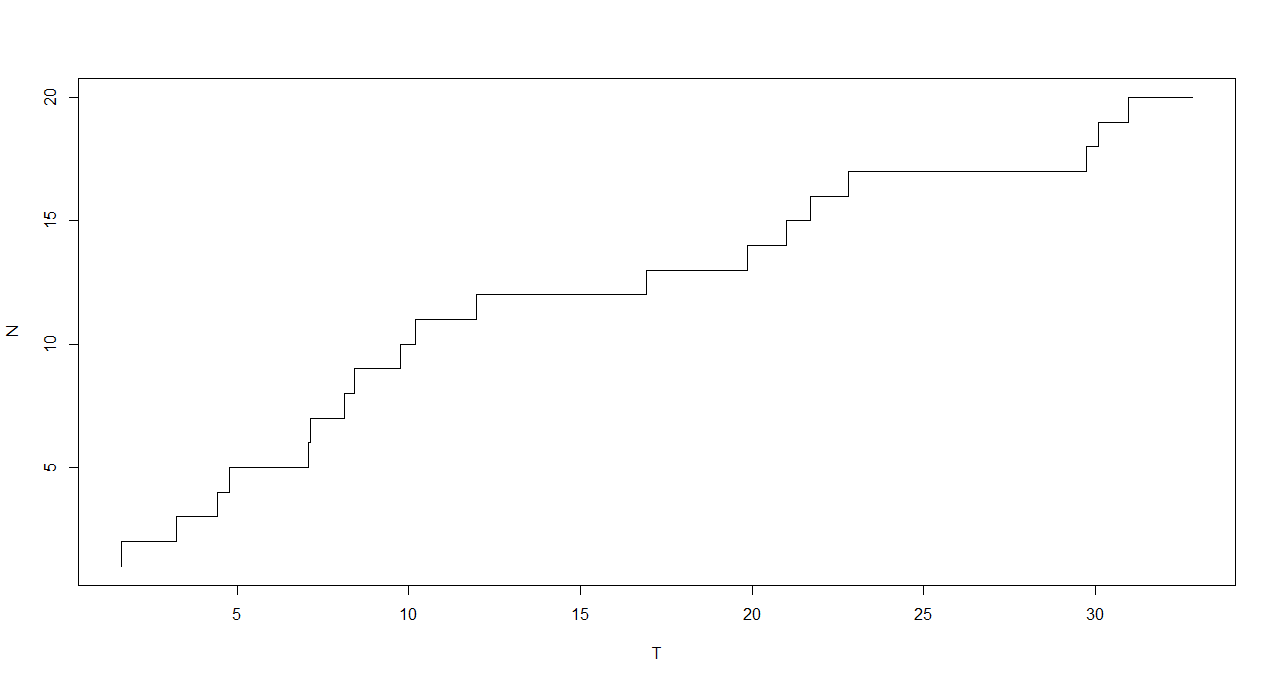
\includegraphics[width=0.7\textwidth]{simexp.png}
\caption{ Simulaci\'on del proceso Poisson mediante variables exponenciales}
\label{1}
\end{figure}
\begin{figure}
\centering
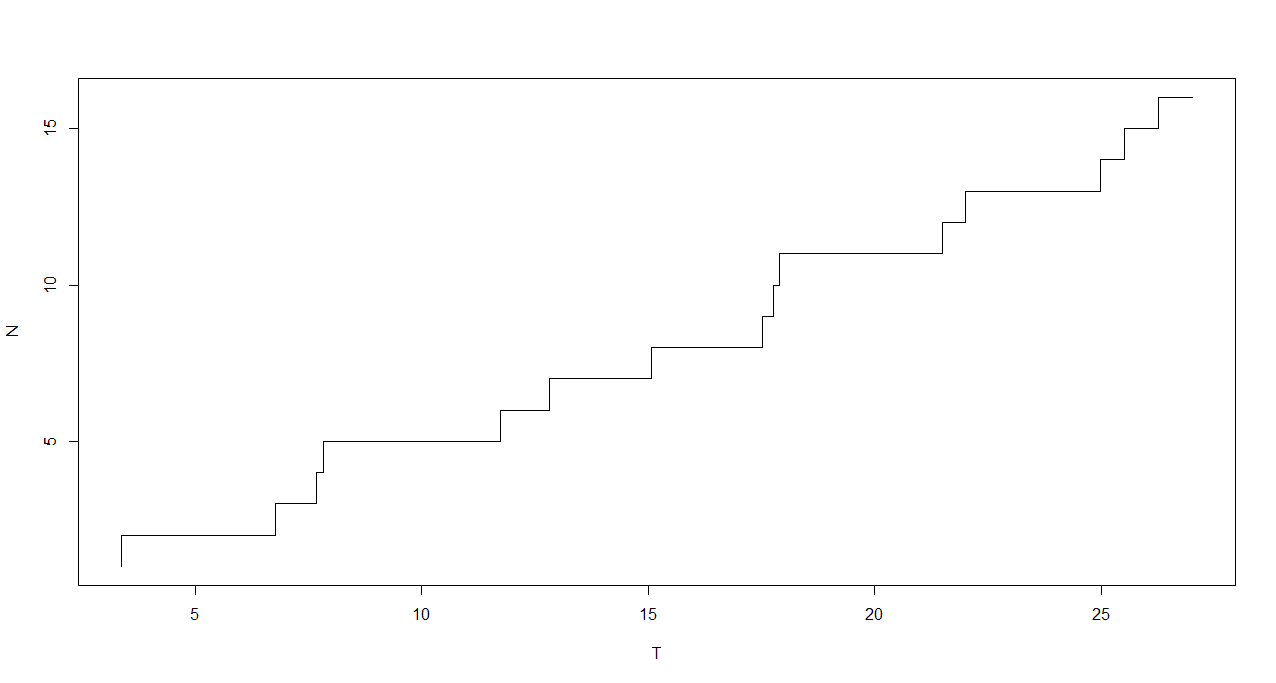
\includegraphics[width=0.7\textwidth]{simpos.png}
\caption{ Simulaci\'on del proceso Poisson mediante una variable Poisson}
\label{2}
\end{figure}
\end{enumerate}
\end{problema}
\begin{problema}
%Simulaci\'on de un proceso Poisson puntual... subordinador...
 Sea $\Xi$ una medida de Poisson aleatoria en $(0,\infty)\times (0,\infty)$ cuya medida de intensidad $\nu$ est\'a dada por $\imf{\nu}{ds,dx}=\indi{s<t}\indi{x>0}C/x^{1+\alpha}\, ds\,dx$. 
 \begin{enumerate}
\item Determine los valores de $\alpha$ para los cuales $\int 1\wedge x\,\imf{\nu}{dx}<\infty$. 
 
\begin{proof}
Tenemos que:
\begin{esn}
\int 1\wedge x\imf{\nu}{ds,dx}=\int_0^t\int_0^1 x C/x^{1+\alpha}dxds + \int_0^t\int_1^\infty  C/x^{1+\alpha}dxds
\end{esn}

Veamos las condiciones para que la primera integral sea finita, primero notemos que $\alpha\neq 1$, ya que en caso contrario tendriamos $ \int_0^1 x C/x^{1+\alpha} dx= \int_0^1  C/x dx=\lim_{x\rightarrow 0}-ln(x)=\infty$.Entonces si $\alpha\neq 1$:
\begin{esn}
\int_0^1 x C/x^{1+\alpha} dx =\frac{C}{1-\alpha} - C\lim_{x \rightarrow 0}\frac{x^{-\alpha+1}}{1-\alpha}.
\end{esn}

Entonces $C\lim_{x \rightarrow 0}\frac{x^{-\alpha+1}}{1-\alpha}$ existe siempre que $\alpha < 1$.
Ahora veamos las condiciones para que la segunda integral se finita, notemos que $\alpha\neq 0$ por el mismo argumento que en el caso anterior. Entonces si $\alpha\neq 0$:

\begin{esn}
\int_1^\infty  C/x^{1+\alpha} dx=\frac{C}{\alpha}-C\lim_{x \rightarrow \infty}\frac{x^{-\alpha}}{\alpha}
\end{esn}
En este caso $\alpha>0$.

Por lo tanto si $\alpha \in (0,1)$ entonces $\int 1\wedge x\,\imf{\nu}{dx}<\infty$.
\end{proof}
Nos restringimos ahora a valores de $\alpha$ para los cuales la integral anterior sea finita. Sean $\imf{f_t}{s,x}=\indi{s\leq t}x$ y $X_t=\Xi f_t$.
 \item Determine los valores  de $\alpha$ para los cuales $X_t<\infty$ para toda $t\geq 0$ casi seguramente.
\begin{proof}
Por proposici\'on vista en clase sabemos que $X_t<\infty$ si  la integral $\int 1 \wedge f_t dv$ es finita, entonces:
\begin{align}
\int 1 \wedge f_t dv&=\int_0^1\int_0^{\infty}\indi{s\leq t}xC/x^{1+\alpha}dsdx + \int_1^\infty\int_0^{\infty} \indi{s\leq t}C/x^{1+\alpha}dsdx \notag \\
&=\int_0^1\int_0^{t}xC/x^{1+\alpha}dsdx + \int_1^\infty\int_0^{t}C/x^{1+\alpha}dsdx \notag \\
&=Ct\paren{\int_0^1 \frac{1}{x^{\alpha}}dx+\int_1^{\infty}\frac{1}{x^{1+\alpha}}} \notag
\end{align}

Analogamente que en el ejercicio anterior $\alpha \in (0,1)$ para que $\int 1 \wedge f_t dv<\infty$. Por lo tanto $X_t<\infty$ casi seguramente si $\alpha \in (0,1)$.
Adem\'as si $\alpha \in (0,1)$ tenemos que:
\begin{esn}
\int 1 \wedge f_t dv =Ct\paren{\frac{1}{1-\alpha}+\frac{1}{\alpha}}=\frac{Ct}{\alpha(1-\alpha)}.
\end{esn}

\end{proof}

 \item Calcule $\esp{e^{-\lambda X_t}}$ y pruebe que $X_{t}$ tiene la misma distribuci\'on que $t^{1/\alpha}X_1$.
 \begin{proof}
Utilizando teorema visto en clase sabemos que:
\begin{esn}
\esp{e^{-\Xi f}}=\exp\paren{-\int\paren{1-e^{-f}}d\nu}
\end{esn}

Entonces:

\begin{esn}
\esp{e^{-\lambda X_t}}=\exp\paren{-\int\paren{1-e^{-\lambda f_t}}d\nu}
\end{esn}


Ahora calculando la integral tenemos que:

\begin{align}
\int\paren{1-e^{-\lambda f_t}}d\nu &= C\int_0^{\infty}\int_0^{t} \paren{1-e^{-\lambda x}} \frac{1}{x^{1+\alpha}}dsdx \notag \\
&=Ct\int_0^{\infty} \paren{1-e^{-\lambda x}}\frac{1}{x^{1+\alpha}}dx \notag \\
&=Ct\int_0^{\infty}\int_0^{x}\lambda e^{-\lambda y}\frac{1}{x^{1+\alpha}}dydx \notag \\
&=Ct\int_0^{\infty}\int_y^{\infty}\frac{\lambda e^{-\lambda y}}{x^{1+\alpha}}dxdy \notag \\
&=\frac{Ct}{\alpha}\int_0^{\infty} \lambda e^{-\lambda y} y^{-\alpha}dy \notag
\intertext{Completando par que nos quede una Gamma:}
&=\frac{Ct\lambda^{\alpha}}{\alpha}\int_0^{\infty}e^{-\lambda y}(\lambda y)^{-\alpha} \lambda dy \notag \\
&=\frac{Ct\lambda^{\alpha}}{\alpha}\Gamma(1-\alpha) \notag
\end{align}

Por lo tanto $\esp{e^{-\lambda X_t}}=\exp\paren{-\frac{C\lambda^{\alpha}\Gamma(1-\alpha)t}{\alpha}}$

Para verificar que tiene la misma distribuci\'on que $t^{1/\alpha}X_1$ nos basta con verificar que   $\esp{e^{-\lambda t^{1/\alpha}X_1}}= \esp{e^{-\lambda X_t}}$. Luego entonces definamos $\phi(\lambda,t)=\esp{e^{-\lambda X_t}}=\exp\paren{-\frac{C\lambda^{\alpha}\Gamma(1-\alpha)t}{\alpha}}$. Evaluando en $t=1$ tenemos que:
\begin{esn}
\phi(\lambda,1)=\esp{e^{-\lambda X_1}}=\exp\paren{-\frac{C\lambda^{\alpha}\Gamma(1-\alpha)}{\alpha}}.
\end{esn}

Evaluando en $\lambda t^{1/\alpha}$:
\begin{esn}
\phi(\lambda t^{1/\alpha},1)=\esp{e^{-\lambda t^{1/\alpha} X_1}}=\exp\paren{-\frac{C(\lambda t^{1/\alpha} )^{\alpha}\Gamma(1-\alpha)}{\alpha}}=\exp\paren{-\frac{C\lambda^{\alpha}\Gamma(1-\alpha)t}{\alpha}}.
\end{esn}

Por lo tanto como $\esp{e^{-\lambda t^{1/\alpha} X_1}}=\esp{e^{-\lambda X_t}}$ entonces $X_t$ se distribuye igual que $t^{1/\alpha}X_1$.
\end{proof}
 \item Diga por qu\'e el siguiente c\'odigo en Octave simula la trayectoria aproximada del proceso $X$ en el intervalo $[0,1]$.
 \end{enumerate}
\end{problema}
\begin{problema}
Pruebe que si $X$ tiene incrementos independientes entonces el proceso $X^t$ dado por $X^t_s=X_{t+s}-X_t$ es independiente de $\F^X_t=\sag{X_s:s\geq 0}$.

Calcular la esperanza y varianza del proceso de Poisson y de Poisson compuesto (en t\'erminos de la intensidad y la distribuci\'on de salto).

\begin{proof}
Como $N_t$ se distribuye Poisson$(\lambda t)$ entonces $\esp{N_t}=\var{N_t}=\lambda t$.

Ahora si tenenemos un proceso Poisson compuesto, $X_t=\sum_{i=0}^{N_t}\xi_i$ donde $\xi_i$ son variables aleatorias independientes e identicamente distribuidas. Entonces:

\begin{align}
\esp{X_t}&=\esp{\sum_{i=0}^{N_t}\xi_i}\notag \\
&=\esp{\espc{\sum_{i=0}^{N_t}\xi_i}{N_t}}\notag \\ &=\esp{\sum_{k=0}^{\infty}\espc{\sum_{i=0}^{N_t}\xi_i}{N_t=k}\indi{N_t=k}}\notag \\
&=\esp{\sum_{k=0}^{\infty}\esp{\sum_{i=0}^{k}\xi_i}\indi{N_t=k}}\notag \\ &=\esp{\sum_{k=0}^{\infty}k\esp{\xi_1}\indi{N_t=k}}\notag \\ &=\esp{\xi_1}\esp{\sum_{k=0}^{\infty}k\indi{N_t=k}} \notag \\
&=\esp{\xi_1}\esp{N_t}\notag \\
&=\esp{\xi_1}\lambda t\notag
\end{align}

Por lo tanto $\esp{X_t}=\esp{\xi_1}\lambda t$.
Ahora calcularemos la varianza:

\begin{align}
\var{X_t}&=\esp{\var{X_t|N_t}}+\var{\espc{X_t}{N_t}} \notag \\
&=\esp{\var{X_t|N_t}}+\var{\esp{\xi_1}N_t}\notag \\
&=\esp{\var{X_t|N_t}}+\esp{\xi_1}^2\var{N_t}\notag \\
&=\esp{\var{X_t|N_t}}+\esp{\xi_1}^2\lambda t \notag
\end{align}

Solo nos falta calcular el primer sumando lo cual lo haremos de la siguiente manera:

\begin{align}
\var{X_t|N_t}&=\espc{X_t^2}{N_t}-\espc{X_t}{N_t}^2\notag \\
&=\espc{X_t^2}{N_t}-{N_t}^2\esp{\xi_i}^2\notag \\
&=\espc{\paren{\sum_{i=0}^{N_t}\xi_i}^2}{N_t}-{N_t}^2\esp{\xi_i}^2\notag \\
&=\sum_{k=0}^{\infty}\espc{\paren{\sum_{i=0}^{N_t}\xi_i}^2}{N_t=k}\indi{N_t=k}-{N_t}^2\esp{\xi_i}^2\notag \\
&=\sum_{k=0}^{\infty}\esp{\paren{\sum_{i=0}^{k}\xi_i}^2}\indi{N_t=k}-{N_t}^2\esp{\xi_i}^2\notag \\
&=\sum_{k=0}^{\infty}\paren{k\esp{\xi_1^2}+k(k-1)\esp{\xi_1}^2}\indi{N_t=k}-{N_t}^2\esp{\xi_i}^2\notag \\
&=N_t\esp{\xi_1^2}+N_t(N_t-1)\esp{\xi_1}^2-{N_t}^2\esp{\xi_i}^2\notag \\
&=N_t\paren{\esp{\xi_1^2}-\esp{\xi_1}^2}\notag \\
&=N_t\paren{\var{\xi_1^2}} \notag
\end{align}

Entonces sustituyendo obtenemos que:
\begin{align}
\var{X_t}&=\esp{N_t\paren{\var{\xi_1^2}}}+\esp{\xi_1}^2\lambda t \notag \\
&=\var{\xi_1^2}\lambda t+\esp{\xi_1}^2\lambda t \notag \\
&=\lambda t \esp{\xi_1^2}\notag
\end{align}

Por lo tanto $\esp{X_t}=\esp{\xi_1}\lambda t$ y $\var{X_t}=\esp{\xi_1^2}\lambda t$.

\end{proof}

Probar que si $X$ es\begin{esn}
\esp{e^{iu Z_t}}=e^{-\lambda t\paren{1-\imf{\psi}{u}}}\quad\text{donde}\quad \imf{\psi}{u}=\esp{e^{iu \xi_1}}.\end{esn}

\begin{proof}

\begin{align}
\esp{e^{iu X_t}}&=\esp{e^{iu \sum_{i=0}^{N_t}\xi_i}}\notag \\
&=\esp{\espc{e^{iu \sum_{i=0}^{N_t}\xi_i}}{N_t}}\notag
\end{align}

Nos enfocaremos en calcular $\espc{e^{iu \sum_{i=0}^{N_t}\xi_i}}{N_t}$:

\begin{align}
\espc{e^{iu \sum_{i=0}^{N_t}\xi_i}}{N_t}&=\sum_{k=0}^{\infty}\espc{e^{iu \sum_{i=0}^{N_t}\xi_i}}{N_t=k} \indi{Nt=k} \notag \\
&=\sum_{k=0}^{\infty}\esp{e^{iu \sum_{i=0}^{k}\xi_i}}\indi{Nt=k} \notag \\
&=\sum_{k=0}^{\infty}\esp{\prod_{i=0}^ke^{iu \xi_i}}\indi{Nt=k}\notag \\
&=\sum_{k=0}^{\infty}\esp{e^{iu \xi_1}}^k\indi{Nt=k} \notag  \\
&=\esp{e^{iu \xi_1}}^{N_t}\notag \\
&=\imf{\psi}{u}^{N_t}\notag
\end{align}

Sustituyendo:
\begin{align}
\esp{e^{iu X_t}} &=\esp{\imf{\psi}{u}^{N_t}}\notag \\
&=\sum_{k=0}^{\infty}\imf{\psi}{u}^k\p(N_t=k)\notag \\
&=\sum_{k=0}^{\infty}\imf{\psi}{u}^k\frac{(\lambda t)^{k}}{k!}e^{-\lambda t}\notag \\
&=e^{-\lambda t}\sum_{k=0}^{\infty}\frac{(\imf{\psi}{u} \lambda t)^{k}}{k!}\notag \\
&=e^{-\lambda t}e^{\imf{\psi}{u} \lambda t}\notag \\
&=e^{-\lambda t\paren{1-\imf{\psi}{u}}}\notag
\end{align}

Por lo  tanto $\esp{e^{iu X_t}}=e^{-\lambda t\paren{1-\imf{\psi}{u}}}$.
\end{proof}



Sea $N$ un proceso de L\'evy tal que $N_t$ tiene distribuci\'on de par\'ametro $\lambda t$. 
\begin{enumerate}
\item Pruebe que casi seguramente las trayectorias de $N$ son no-decrecientes.
\begin{proof}


\begin{align}
\proba{N_{t+s}\geq N_t}&=\proba{N_{t+s}-N_t\geq 0}\notag \\
&=\proba{N_{t}-N_0\geq 0}\notag \\
&=\proba{N_t\geq 0}=1 \notag
\end{align}
ya que por hip\'otesis sabemos que $N_t$ tiene distribuci\'on de par\'ametro $\lambda t$.

Por lo tanto $N_{t+s}\geq N_t$ casi seguramente.
\end{proof}

\item Sea $\Xi$ la \'unica medida en $\mc{B}_{\re_+}$ tal que $\imf{\Xi}{[0,t]}=N_t$. Pruebe que $\Xi$ es una medida de Poisson aleatoria de intensidad $\lambda \cdot\leb$.
\begin{proof}
Por proposici\'on 4.5  de las notas se obtiene el resultado.
\end{proof}

\item Concluya que $N$ es un proceso de Poisson de intensidad $\lambda$.

\begin{proof}
El inciso anterior nos ind\'ica que $N$ es un proceso de conteo y adem\'as como es proceso de Levy por teorema visto en clase $N$ es un proceso de Poisson de intensidad $\lambda$.
\end{proof}

\end{enumerate}
\end{problema}

\begin{problema}
Sea $P_t$ la probabilidad de transici\'on en $t$ unidades de tiempo para el proceso de Poisson de par\'ametro $\lambda$. 

Al utilizar el teorema del biniomio, pruebe directamente que las probabilidades de transici\'on del proceso de Poisson satisfacen las ecuaciones de Chapman-Kolmogorov $P_{t+s}=P_tP_s$. D\'e adem\'as un argumento probabil\'istico, basado en condicionar con lo que sucede al tiempo $s$, para probar dicha ecuaci\'on. 

Sea\begin{esn}
\imf{Q}{i,j}=\begin{cases}
-\lambda&j=i\\
\lambda&j=i+1\\
0&j\neq i,i+1
\end{cases}.
\end{esn}Pruebe directamente que se satisfacen las ecuaciones de Kolmogorov\begin{equation*}
%\label{CKEquationsForPoisson}
\frac{d}{dt}\imf{P_t}{i,j}=\imf{QP_t}{i,j}=\imf{P_tQ}{i,j},
\end{equation*}donde $QP_t$ es el producto de las matrices $Q$ y $P_t$.

\begin{proof}
Como estamos en un proceso Poisson de par\'amettro $\lambda$ tenemo que:
\begin{esn}
P_t(i,j)=\p(N_t=j-i)=e^{-\lambda t}\frac{(\lambda t)^{j-i}}{(j-i)!} 
\end{esn}

Entonces:

\begin{align}
P_{t+s}(i,j)&=e^{-\lambda (t+s)}\frac{(\lambda (t+s))^{j-i}}{(j-i)!}\notag \\
&=e^{-\lambda (t+s)}\frac{\lambda^{j-i}(t+s)^{j-i}}{(j-i)!}\notag \\
&=e^{-\lambda (t+s)}\frac{\lambda^{j-i}\sum_{k=0}^{j-i}\binom{j-i}{k}s^kt^{j-i-k}}{(j-i)!}\notag \\
&=e^{-\lambda (t+s)}\lambda^{j-i}\sum_{k=0}^{j-i}\frac{s^kt^{j-i-k}}{(k)!(j-i-k)!}.\notag
\end{align}

Ahora veamos el producto de matrices entrada por entrada:

\begin{align}
(P_tP_s)(i,j)&=\sum_{k=0}^{\infty}P_t(i,k)P_s(k,j)\notag \\
&=\sum_{k=0}^{\infty}e^{-\lambda t}\frac{(\lambda t)^{k-i}}{(k-i)!} e^{-\lambda s}\frac{(\lambda s)^{j-k}}{(j-k)!}\notag
\intertext{Como el proceso Poisson es creciente tenemos que $i\leq k\leq j$:}
&=e^{-\lambda (t+s)}\lambda^{j-i}\sum_{k=i}^{j}\frac{s^{j-k}t^{k-i}}{(k-i)!(j-k)!}\notag 
\intertext{Haciendo  $h=k-i$:}
&=e^{-\lambda (t+s)}\lambda^{j-i}\sum_{h=0}^{j-i}\frac{s^{j-h-i}t^{h}}{(h)!(j-h-i)!}\notag
\end{align}

Por lo tanto:
\begin{esn}
P_{s+t}=P_sP_t.
\end{esn}

El argumento probabilistico es el siguiente:
\begin{align}
P_{t+s}(i,j)&=\proba{N_{t+s}=j-i}\notag \\
&=\sum_{k=0}^{\infty}\proba{N_{t+s}=j-i,N_s=k}
\intertext{Como $N_{t+s}\geq N_s$ entonces $j-i\geq k$:}
&=\sum_{k=0}^{j-i}\proba{N_{t+s}=j-i,N_s=k}\notag \\
&=\sum_{k=0}^{j-i}\proba{N_{t+s}-N_s=j-i-k,N_s=k}\notag
\intertext{Haciendo h=$k+i$:}
&=\sum_{h=i}^{j}\proba{N_{t+s}-N_s=j-h,N_s=h-i}\notag \\
&=\sum_{h=i}^{j}\proba{N_{t+s}-N_s=j-h}\proba{N_s=h-i}\notag \\
&=\sum_{h=i}^{j}\proba{N_{t}=j-h}\proba{N_s=h-i}\notag \\
&=\sum_{h=i}^{j}P_s(i,h)P_t(h,j) \notag \\
&=(P_sP_t)(i,j). \notag
\end{align}

Ahora probaremos que se cumplen las ecuaciones de Kolmogorov. Calculando la derivada:


\begin{esn}
\frac{d}{dt}\imf{P_t}{i,j}=\frac{d}{dt}\frac{(\lambda t)^{j-i}}{(j-i)!}e^{-\lambda t}=-\lambda P_t(i,j)+\lambda P_t(i+1,j)
\end{esn}

Ahora fijemonos en la multiplicaci\'on de matrices:
\begin{align}
\imf{QP_t}{i,j}&=\sum_{k=0}^{\infty}Q(i,k)P_t(k,j)\notag \\
&=Q(i,i)P_t(i,j)+Q(i,i+1)P_t(i+1,j)\notag \\
&=-\lambda P_t(i,j)+\lambda P_t(i+1,j)\notag \\
&=\frac{d}{dt}\imf{P_t}{i,j}. \notag
\end{align}

Ahora notemos que:
\begin{align}
\imf{P_tQ}{i,j}&=\sum_{k=0}^{\infty}P_t(i,k)Q(k,j)\notag \\
&=P_t(i,j)Q(j,j)+P_t(i,j-1)Q(j-1,j)\notag \\
&=-\lambda P_t(i,j)+\lambda P_t(i,j-1)\notag \\
&=-\lambda P_t(i,j)+\lambda\proba{N_t=j-1-i} \notag \\
&=-\lambda P_t(i,j)+\lambda\proba{N_t=j-(i+1)} \notag \\
&=-\lambda P_t(i,j)+\lambda P_t(i+1,j)\notag \\
&=\frac{d}{dt}\imf{P_t}{i,j}\notag
\end{align}

Por lo tanto se cumplen las ecuaciones backward y forward de Kolmogorov.
\end{proof}

\end{problema}

\begin{problema}[Tomado del examen general de probabilidad del Posgrado en Ciencias Matem\'aticas, UNAM, \href{http://www.posgradomatematicas.unam.mx/contenidoEstatico/archivo/files/pdf/Examenes_Generales/Probabilidad/Probabilidad2011-1.pdf}{Febrero 2011}]
Una planta de producci\'on toma su energ\'ia de dos generadores. La cantidad de generadores al tiempo $t$ est\'a representado por una cadena de Markov a tiempo continuo $\set{X_t,t\geq 0}$ con espacio de estados $E=\set{0,1,2}$ y matriz infinit\'esimal $Q$ dada por\begin{esn}
Q=\begin{pmatrix}
-6&6&0\\
1&-7&6\\
0&2&-2
\end{pmatrix}.
\end{esn}
\begin{enumerate}
\item Encuentre la matriz de transici\'on de la cadena de Markov de los estados distintos que toma $X$, clasifique los estados, diga si existe una \'unica distribuci\'on invariante y en caso afirmativo, encu\'entrela. Calcule expl\'icitamente las potencias de la matriz de transici\'on. (Recuerde que de ser posible diagonalizar, esta es una buena estrategia.)
\begin{proof}
Sabemos que $-c(x)=Q(x,x)$ y que $\alpha(x,y)=Q(x,y)=c(x)P(x,y)$, obtenrmos que la matriz de transci\'on es
\begin{esn}
P=\begin{pmatrix}
0&1&0\\
1/7&0&6/7\\
0&1&0
\end{pmatrix}
\end{esn}

Todos los estados son recurrentes y $P$ es irrecucible. Por lo tanto existe la distribuci\'on invariante:

\begin{esn}
\begin{pmatrix}
\pi_1& \pi_2& \pi_3
\end{pmatrix}
\begin{pmatrix}
0&1&0\\
1/7&0&6/7\\
0&1&0
\end{pmatrix}
=\begin{pmatrix}
\pi_1&\pi_2& \pi_3
\end{pmatrix}
\end{esn}

Con la condici\'on de que $\pi_1+\pi_2+\pi_3=1$ entonces $\pi=(1/14,1/2,3/7)$. Como $P$ tiene distribuci\'on invariante entonces $P_t$ tiene distibuci\'on invariante. Caculando la distribuci\'on invariante de $P_t$:

\begin{esn}
\begin{pmatrix}
6\pi_1& 7\pi_2& 2\pi_3
\end{pmatrix}
\begin{pmatrix}
0&1&0\\
1/7&0&6/7\\
0&1&0
\end{pmatrix}
=\begin{pmatrix}
6\pi_1&7\pi_2& 2\pi_3
\end{pmatrix}
\end{esn}

Con la condici\'on de que $\pi_1+\pi_2+\pi_3=1$ entonces $\pi=(1/25,6/25,18/25)$.
Para encontrar $P^n$ hay que diagonalizar:

\begin{esn}
P=\frac{1}{14}\begin{pmatrix}
-6&1&-1\\
0&1&1\\
1&1&-1
\end{pmatrix}\begin{pmatrix}
0&0&0\\
0&1&0\\
0&0&-1
\end{pmatrix}
\begin{pmatrix}
-2&0&2\\
1&7&6\\
-1&7&-6
\end{pmatrix}
\end{esn}

Por lo tanto:

\begin{esn}
P^n=\frac{1}{14}\begin{pmatrix}
-6&1&-1\\
0&1&1\\
1&1&-1
\end{pmatrix}\begin{pmatrix}
0&0&0\\
0&1&0\\
0&0&(-1)^n
\end{pmatrix}
\begin{pmatrix}
-2&0&2\\
1&7&6\\
-1&7&-6
\end{pmatrix}
\end{esn}
Por lo tanto:
\begin{esn}
P^{2n+1}=\begin{pmatrix}
0&1&0\\
1/7&0&6/7\\
0&1&0
\end{pmatrix}
\end{esn}
 y 
\begin{esn}
P^{2n}=\begin{pmatrix}
1/7&0&6/7\\
0&1&0\\
1/7&0&6/7
\end{pmatrix}
\end{esn}
\end{proof}
\item ?`Cu\'al es la probabilidad de que ambos generadores est\'en trabajando al tiempo $t$ si s\'olo uno trabaja al tiempo cero?
\begin{proof}
Calcualremos $P_t$ para encontrar la probabilidad deseada. Sabemos que $P_t=e^{Qt}$, primero diagonalizaremos $Q$.
\begin{esn}
Q=\frac{1}{25}\begin{pmatrix}
1&18&-6\\
1&3&4\\
1&-2&-1
\end{pmatrix}\begin{pmatrix}
0&0&0\\
0&-5&0\\
0&0&-10
\end{pmatrix}
\begin{pmatrix}
1&6&18\\
1&1&-2\\
-1&4&-3
\end{pmatrix}
\end{esn}

Entonces:

\begin{esn}
P_t=\frac{1}{25}\begin{pmatrix}
1&18&-6\\
1&3&4\\
1&-2&-1
\end{pmatrix}\begin{pmatrix}
1&0&0\\
0&e^{-5t}&0\\
0&0&e^{-10t}
\end{pmatrix}
\begin{pmatrix}
1&6&18\\
1&1&-2\\
-1&4&-3
\end{pmatrix}
\end{esn}

Por lo tanto $P_t(1,2)=\frac{1}{25}(18-6e^{-5t}-12e^{-10t})$
\end{proof}
\item Si $\rho_2$ denota la primera vez que ambos generadores est\'an trabajando al mismo tiempo, encuentre la distribuci\'on de $\rho_2$ cuando s\'olo un generador est\'a trabajando al tiempo cero.
\begin{proof}
Para encontrar a $\rho_2$ hacemos al segundo estado absorbente, entonces la matriz $Q$ se transforma de la siguiente manera:

\begin{esn}
Q=\begin{pmatrix}
-6&6&0\\
1&-7&6\\
0&0&0
\end{pmatrix}.
\end{esn}
\end{proof}

Diagonalizando $Q$ para encontrar $P_t$ tenemos que:

\begin{esn}
Q=\frac{1}{5}\begin{pmatrix}
1&3&-2\\
1&1&1\\
1&-0&0
\end{pmatrix}\begin{pmatrix}
0&0&0\\
0&-4&0\\
0&0&-9
\end{pmatrix}
\begin{pmatrix}
0&0&5\\
1&2&-3\\
-1&3&-2
\end{pmatrix}
\end{esn}

Calculando $P_t$ mediante la ecuaci\'on forward de Kolmogorov:

\begin{esn}
P_t=\frac{1}{5}\begin{pmatrix}
1&3&-2\\
1&1&1\\
1&-0&0
\end{pmatrix}\begin{pmatrix}
1&0&0\\
0&e^{-4t}&0\\
0&0&e^{-9t}
\end{pmatrix}
\begin{pmatrix}
0&0&5\\
1&2&-3\\
-1&3&-2
\end{pmatrix}
\end{esn}

Como el estado 2 es absorbente entonces:
\begin{esn}
\proba{\rho_2 \leq t}=P_t(1,2)=\frac{1}{5} (5-3e^{-4t}-2e^{-9t})
\end{esn}

\item Encuentre la proporci\'on de tiempo asint\'otica en que los dos generadores est\'an trabajando. Si cada generador produce 2.5 MW de energ\'ia por unidad de tiempo, ?`Cu\'al es la cantidad promedio de energ\'ia producida a largo plazo por unidad de tiempo?
\begin{proof}
La proporci\'on de tiempo asint\'otica de que ambos generadores esten trabajando es: $\pi_3=18/25$.
La cantidad promedio es $5*\pi_3+2.5*\pi_2=5*18/25+2.5*6/25=4.2$.
\end{proof}
\end{enumerate}
\end{problema}
\begin{problema}[Procesos de ramificaci\'on a tiempo continuo]
Sea $\mu$ una distribuci\'on en $\na$. A $\mu_k$ lo interpretamos como la probabilidad de que un individuo tenga $k$ hijos. Nos imaginamos la din\'amica de la poblaci\'on como sigue: a tasa $\lambda$, los individuos de una poblaci\'on se reproducen. Entonces tienen $k$ hijos con probabilidad $\mu_k$. Se pueden introducir dos modelos: uno en que el individuo que se reproduce es retirado de la poblaci\'on (nos imaginamos que muere) y otro en que no es retirado de la poblaci\'on (por ejemplo cuando se interpreta a la poblaci\'on como especies y a sus descendientes como mutaciones). En el caso particular del segundo modelo en que $\mu_1=1$, se conoce como proceso de Yule. 
\begin{enumerate}
\item Especifique un modelo de cadenas de Markov a tiempo continuo para cada uno de los modelos anteriores. A estos procesos se les conoce como procesos de ramificaci\'on a tiempo continuo.
\begin{proof}


Si empezamos con $k$ hijos la distribuci\'on inicial sera $X_0=k$. Para el primer caso, la muerte de un individuo y que tenga $n$ hijos es equivalente a que no se muera y tenga $n-1$ hijos, adem\'as eliminaremos el caso en el que el individuo tiene 1 hijo debido a que no cambio de estado. Entonces $\alpha(0,x)=0$, $\alpha(x,y)=0$ si $y<x-1$, $\alpha(x,x)=0$, $\alpha(x,x-1)=\lambda x \mu_0$ y $\alpha(x,x+k)=\lambda x\mu_{k+1}$ para toda $k\in \na$.

En el segundo caso no hay muerte y adem\'as tambi\'en eliminaremos el caso en el que el individuo no tiene hijos de a que tiene que cambiar de estado , entonces $\alpha(0,x)=0$, $\alpha(x,y)=0$ si $y\leq x$ y $\alpha(x,x+k)=\lambda x \mu_k$ para toda $k\in \na$.

De aqui podemos calcular la matriz $P$, $c(x)=\sum_{y\in E} \alpha(x,y)=\lambda$ y $P(x,y)=\alpha(x,y)/c(x)$.

Por lo tanto para el primer caso tenemos que:

\begin{esn}
P=\begin{pmatrix}
1&0 & 0 & 0 &\ldots \\
\mu_0&0&\mu_2&\mu_3&\ldots \\
0&\mu_0&0&\mu_2&\ldots \\
\vdots &\vdots &\vdots &\vdots &\ddots 
\end{pmatrix}
\end{esn}
y para el segundo caso:
\begin{esn}
P=\begin{pmatrix}
1&0 & 0 & 0 &\ldots \\
0&0&\mu_1&\mu_2&\ldots \\
0&0&0 &\mu_1 &\ldots \\
\vdots &\vdots &\vdots &\vdots &\ddots 
\end{pmatrix}.
\end{esn}

Entonces sean $S_1,S_2,...$ variables aleatorias exponenciales de par\'amaetro 1 y una cadena de markov $Z_n$ a tiempo discreto con matriz de transici\'on $P$. Definimos $T_0=0$ y $T_{n+1}=T_n+S_n/c(Z_n)$, definiendo a $X_t=Z_n$ si $[T_n,T_{n+1}]$ entonces $X_t$ es una cadena de Markov a tiempo continuo.

\end{proof}
Nuestro primer objetivo ser\'a encontrar una relaci\'on entre procesos de ramificaci\'on a tiempo continuo y procesos de Poisson compuestos. Sea $N$ un proceso de Poisson  y $S$ una caminata aleatoria independiente de $N$ tal que $\proba{S_1=j}=\mu_{j-1}$ \'o $\mu_{j}$ dependiendo de si estamos en el primer caso o en el segundo. Sea $k\geq 0$ y definamos a $X_t=k+S_{N_t}$.

\item Diga brevemente por qu\'e $X$ es una cadena de Markov a tiempo continuo e identifique su matriz infinitesimal para ambos modelos.

\begin{proof}

Si definimos al proceso $W_n=X_{T_n}=k+S_n$. Mostraremos que $W_n$ es una cadena de Markov a tiempo discreto, sean $\epsilon_i$ las variables aleatorias independientes de la caminata aleatoria, entonces:

\begin{align}
&\probac{W_n=i_n}{W_{n-1}=i_{n-1}, ..., W_1=i_1} \notag \\
&=\frac{\proba{W_n=i_n,W_{n-1}=i_{n-1}, ..., W_1=i_1}}{\proba{W_{n-1}=i_{n-1}, ..., W_1=i_1}} \notag \\
&=\frac{\proba{W_n-W_{n-1}=i_n-i_{n-1}, ..., W_2-W_1=i_2-i_1,W_1=i_1}}{\proba{W_{n-1}-W_{n-2}=i_{n-1}-i_{n-2}, ..., W_2-W_1=i_2-i_1,W_1=i_1}}\notag \\
&=\frac{\proba{\epsilon_n=i_n-i_{n-1}, ..., \epsilon_2=i_2-i_1,\epsilon_1=i_1-k}}{\proba{\epsilon_{n-1}=i_{n-1}-i_{n-2}, ..., \epsilon_2=i_2-i_1,\epsilon_1=i_1-k}}\notag \\
&=\frac{\proba{\epsilon_n=i_n-i_{n-1}} ...\proba{\epsilon_2=i_2-i_1}\proba{\epsilon_1=i_1-k}}{\proba{\epsilon_{n-1}=i_{n-1}-i_{n-2}} ...\proba{B_2=i_2-i_1}\proba{B_1=i_1-k}}\notag \\
&=\mu_{i_n-i_{n-1}} \notag \\
&=\probac{W_n=i_n}{W_{n-1}=i_n-1} \notag
\end{align}

Ademas los tiempos $T_n-T_{n-1}$ se distribuyen $exp(\lambda)$ por ser los mismos del Proceso Poisson. Por lo tanto $X_t$ es una cadena de Markov a tiempo continuo.

Para el primer caso la matriz infinitesimal esta dada por (suponiendo que $\mu_1=0$):

\begin{esn}
Q=\begin{pmatrix}
\ddots&\vdots &\vdots & \vdots & \vdots &\ldots \\
\ldots& \lambda\mu_0&-\lambda&\lambda\mu_2&\lambda\mu_3&\ldots \\
\ldots & 0&2\lambda\mu_0&-2\lambda&2\lambda\mu_2&\ldots \\
\ldots & 0&0& 3\lambda\mu_0&-3\lambda&3\lambda\mu_2&\ldots \\
\vdots &\vdots & \vdots &\vdots &\vdots &\ddots
\end{pmatrix}
\end{esn}
y para el segundo caso (suponiendo que $\mu_0=0$):
\begin{esn}
Q=\begin{pmatrix}
0&0 &0 & 0 & 0 &\ldots \\
0&-\lambda& \lambda\mu_1&\lambda\mu_2&\lambda\mu_3&\ldots \\
0 & 0&-2\lambda &2\lambda\mu_1&2\lambda\mu_2&\ldots \\
0 & 0&0& -3\lambda& 3\lambda\mu_1&3\lambda\mu_2&\ldots \\
\vdots &\vdots & \vdots &\vdots &\vdots &\ddots
\end{pmatrix}
\end{esn}
\end{proof}

Sea ahora $\tau=\min\set{t\geq 0: X_t=0}$ y $Y_t=X_{t\wedge \tau}$. 

\item Argumente por qu\'e $Y$ es una cadena de Markov a tiempo continuo e identifique su matriz infinitesimal.
\begin{proof}
En el segundo caso tenemos que $X_t=Y_t$ ya que la poblaci\'on nunca llega al estado 0. Para el primer caso
sus tiempos de salto siguen siendo independientes  y adem\'as al llegar al estado $0$ el proceso se quda ah\'i, por lo cual el estado = se convierte en estado absorbente. Por lo tanto el proceso $Y_t$ es un proceso de Markov con matriz infintesimal:
\begin{esn}
Q=\begin{pmatrix}
0&0 &0 & 0 & 0 &0 \\
\ldots& \lambda\mu_0&-\lambda&\lambda\mu_2&\lambda\mu_3&\ldots \\
\ldots & 0&2\lambda\mu_0&-2\lambda&2\lambda\mu_2&\ldots \\
\ldots & 0&0& 3\lambda\mu_0&-3\lambda&3\lambda\mu_2&\ldots \\
\vdots &\vdots & \vdots &\vdots &\vdots &\ddots
\end{pmatrix}.
\end{esn}



\end{proof}
\item Argumente por qu\'e existe un \'unico proceso $Z$ que satisface\begin{esn}
Z_t=Y_{\int_0^t Z_s\, ds}
\end{esn}y que dicho proceso es un proceso de ramificaci\'on a tiempo continuo. Sugerencia: Recuerde que las trayectorias de $Y$ son constantes por pedazos.

\begin{proof}
Construiremos $Z$ de manera que cumpla la hip\'otesis. Como $Y_t$ es un proceso constante por pedazos. Nos basta con verificar  donde $Y_t$ cambia, el primer cambio se da em $T_1$, por lo que si $t<T_1$ entonces $Y_t$ integra $kt$. Entonces  para $t<T_1 /k$ definfimos $Z_t=k$.Por lo tanto $\int_0^t Z_s ds=kt<T_1$. Por lo tanto $Y_{\int_0^t Z_s ds}=k=Z_t$.

Para el segundo salto de $Y_t$, el cual se obtiene en $T_2$, tenemos que $Y_t=k+S_1$ cuando $t\in [T_1,T_2)$. Entonces para $t\in [T_1,T_2)$ queremos que $Z_t=k+S_1=Y_{ \int_0^{\frac{T_1}{k}} k\, ds+\int_{\frac{T_1}{k}}^{t}k+S_1}$. Entonces necesitamos que:
\begin{esn}
T_1\leq \int_0^{\frac{T_1}{k}} k\, ds+\int_{\frac{T_1}{k}}^{t}k+S_1< T_2
\end{esn}
Desarrolando tenemos que:
\begin{esn}
\frac{T_1}{k}\leq t < \frac{T_1}{k}+\frac{T_2-T_1}{k+S_1}
\end{esn}


Por lo tanto $Z_t=k+S_1$ cuando $t\in [\frac{T_1}{k}, \frac{T_1}{k}+\frac{T_2-T_1}{k+S_1})$.

Siguiendo el procedimiento obtenemos que en el $n$-\'esimo salto del proceso $Y_t$ toma lugar en $T_n$ y $Y_t=k+S_{n-1}$ en $[T_{n-1},T_n)$. Entonces para que $Z_t=Y_{\int_0^t Z_s ds}$, necesitamos que:
\begin{esn}
T_{n-1}\leq\int_0^{\frac{T_1}{k}} kds + \int_{\frac{T_1}{k}}^{\frac{T_1}{k}+\frac{T_2-T_1}{k+S_1}}k+S_1+...+\int_{\frac{T_1}{k}+...+\frac{T_{n-1}-T_{n-2}}{k+S_{n-2}}}^{t}k+S_{n-1}< T_n
\end{esn}

Esto implica que:
\begin{esn}
\frac{T_1}{k}+ \frac{T_2-T_1}{k+S_1}+...+\frac{T_{n-1}-T_{n-2}}{k+S_{n-2}}\leq t< \frac{T_1}{k}+ \frac{T_2-T_1}{k+S_1}+...+\frac{T_{n}-T_{n-1}}{k+S_{n-1}}
\end{esn}

Por lo tanto $Z_t=k+S_{n-1}=Y_{\int_0^t Z_s\, ds}$ si $t\in[\frac{T_1}{k}+...+\frac{T_{n-1}-T_{n-2}}{k+S_{n-2}},\frac{T_1}{k}+...+\frac{T_{n}-T_{n-1}}{k+S_{n-1}})$
Por lo tanto $Z_t=k+S_{n-1}$ si $t\in[A_{n-1},A_n)$ donde:

\begin{esn}
A_n=\frac{T_1}{k}+\frac{T_{2}-T_{1}}{k+S_{1}}+...+\frac{T_{n}-T_{n-1}}{k+S_{n-1}}
\end{esn}

Notemos que:
\begin{esn}
A_n-A_{n-1}= \frac{T_n-T_{n-1}}{k+S_{n-1}}
\end{esn}

Como $T_i$ proviene de un proceso Poisson $N$ entonces $T_n-T_{n-1}$ se distribuye exponencial $\lambda$. Por lo tanto $\frac{T_n-T_{n-1}}{k+S_{n-1}}$ se distribuye exponencial $\lambda(k+S_{n-1})$. Por lo tanto $Z_t$ es una cadena de Markov a tiempo continuo. Por lo tanto $Z_t$ es un proceso de ramificaci\'on.

\end{proof}

Ahora nos enfocaremos en el proceso de Yule. 

\item Escriba las ecuaciones backward de Kolmogorov para las probabilidades de transici\'on $\imf{P_t}{x,y}$. Al argumentar por qu\'e $\imf{P_{t}}{x,x}=e^{-\lambda x}$, resuelva las ecuaciones backward por medio de la t\'ecnica de factor integrante (comenzando con $\imf{P_t}{x,x+1}$) y pruebe que\begin{esn}
\imf{P_t}{x,y}=\binom{y-1}{y-x} e^{-\lambda x t}\paren{1-e^{-\lambda t}}^{y-x}.
\end{esn}

\begin{proof}
Nos enfocaremos en el segundo caso ya que en el primer caso si $\mu_1=1$ entonces tenemos un proceso constante ya que siempre que un individuo se reproduce es retirado de la poblaci\'on y con probabilidad 1 tiene un hijo.

Las ecuaciones backward son:
\begin{esn}
\frac{d}{dt}\imf{P_t}{x,y}=\sum_{s \in E}Q(x,s)P_t(s,y)
\end{esn}


Luego entonces para el segundo caso se tiene que la matriz infinitesimal esta dada por:

\begin{esn}
Q(x,y)=\begin{cases}
\lambda x &y = x+1 \\
-\lambda x & x=y
\end{cases}
\end{esn}

Entonces:
\begin{esn}
\frac{d}{dt}\imf{P_t}{x,y}=\lambda x P_t(x+1,y)-\lambda x P_t(x,y).
\end{esn}

Para el caso $x=y$ tenemos que:

\begin{align}
\frac{d}{dt}\imf{P_t}{x,x}&=-\lambda x P_t(x,x) \notag \\
\imf{P_t}{x,x}&=e^{-\lambda x  t}=\binom{x-1}{x-x} e^{-\lambda x t}\paren{1-e^{-\lambda t}}^{x-x}
\end{align}

Si $x<y$ entonces $y=x+k$, resolveremos las utilizando inducci\'on sobre $k$. Caso $k=1$
\begin{esn}
\frac{d}{dt}\imf{P_t}{x,x+1}=\lambda x P_t(x+1,x+1)-\lambda x P_t(x,x+1)
\end{esn}
Como $P_t(x+1,x+1)=e^{-\lambda (x+1)t}$ entonces:
\begin{esn}
\frac{d}{dt}\imf{P_t}{x,x+1}=\lambda x e^{-\lambda (x+1)t}-\lambda x P_t(x,x+1)
\end{esn}

Mutiplicando por el factor integrante $e^{\lambda xt}$:
\begin{esn}
\frac{d}{dt}\paren{e^{\lambda xt}P_t(x,x+1)}=\lambda x e^{-\lambda t}
\end{esn}

Integrando  y utilizando la condici\'on inicial de $P_0(x,x+1)=0$:
\begin{esn}
e^{\lambda xt}P_t(x,x+1)=\int_0^t\lambda x e^{-\lambda s}ds=x(1-e^{\lambda t})
\end{esn}

Por lo tanto:
\begin{esn}
P_t(x,x+1)=xe^{-\lambda xt}(1-e^{\lambda t})=\binom{x}{1} e^{-\lambda x t}\paren{1-e^{-\lambda t}}^{x+1-x}.
\end{esn}

Supongamos que la igualdad es v\'alida para $y=x+k$ y demostremos que es v\'alida para $y=x+k+1$. Entonces:
\begin{esn}
\frac{d}{dt}\imf{P_t}{x,x+k+1}=\lambda xP_t(x+1,x+k+1)-\lambda xP_t(x,x+k+1)
\end{esn}
Por hip\'otesis de inducci\'on tenemos que:
\begin{esn}
P_t(x+1,x+k+1)=P_t((x+1),(x+1)+k)=\binom{x+k}{k}e^{-\lambda (x+1) t}\paren{1-e^{-\lambda t}}^{k}
\end{esn}

Entonces:
\begin{esn}
\frac{d}{dt}\imf{P_t}{x,x+k+1}=\lambda x \binom{x+k}{k} e^{-\lambda (x+1) t}\paren{1-e^{-\lambda t}}^{k}-\lambda x P_t(x,x+k+1)
\end{esn}
Multiplicando por el factor integrante tenemos que:
\begin{esn}
\frac{d}{dt}\paren{e^{\lambda xt} \imf{P_t}{x,x+k+1}}=\lambda x \binom{x+k}{k} e^{-\lambda t}\paren{1-e^{-\lambda t}}^{k}
\end{esn}
Integrando 
\begin{esn}
\imf{P_t}{x,x+k+1}=\frac{x}{k+1}\binom{x+k}{k}e^{-\lambda xt} \paren{1-e^{-\lambda t}}^{k+1}.
\end{esn}

Por lo tanto:
\begin{esn}
\imf{P_t}{x,x+k+1}=\binom{x+k}{k+1}e^{-\lambda xt} \paren{1-e^{-\lambda t}}^{k+1}
\end{esn}

Por lo tanto la form\'ula es v\'alida para $k+1$.

Por lo tanto:
\begin{esn}
\imf{P_t}{x,y}=\binom{y-1}{y-x} e^{-\lambda x t}\paren{1-e^{-\lambda t}}^{y-x}
\end{esn}

\end{proof}
\item Al utilizar la f\'ormula para la esperanza de una variable binomial negativa, pruebe que\begin{esn}
\imf{\se_x}{Z_t}= xe^{\lambda t}.
\end{esn}
\begin{proof}

Por lo anterior sabemos que condicionado al que el proceso inicia en $x$, $Z_t$ se distribuye binomial negativa con par\'ametros $p=e^{-\lambda t}$ y $r=x$.

Por lo tanto:
\begin{esn}
\imf{\se_x}{Z_t}=\frac{x}{e^{-\lambda t}}=xe^{\lambda t}
\end{esn}

\end{proof}


\item Pruebe que $e^{-\lambda t}Z_t$ es una martingala no-negativa y que por lo tanto converge casi seguramente a una variable aleatoria $W$.
\begin{proof}
\begin{itemize}
\item Utlizando la filtracion natural $e^{-\lambda t}Z_t$ es $\F_t$-m\'edible.
\item Utilizando el inciso anterior $e^{-\lambda t}Z_t\in L_1$
\item Propiedad de juego justo, sea $s\leq t$:
\begin{align}
\espc{e^{-\lambda t}Z_t}{\F_s}&=e^{-\lambda t}\espc{Z_t}{\F_s}\notag
\intertext{Utilizando la propiedad de Markov:}
&=e^{-\lambda t}\imf{\se_{Z_{s}}}{Z_{t-s}}\notag
\intertext{Utilizando el ejercicio anterior:}
&=e^{-\lambda t}Z_s e^{-\lambda (t-s)} \notag \\
&=e^{-\lambda s}Z_s. \notag
\end{align}
\end{itemize}

Por lo tanto $e^{-\lambda t}Z_t$ es martingala.

Por lo tanto por ser martingala no negativa por el teorema de convergencia de martingalas el preoceso converge a una variable aleatoria $W$ casi seguramente.
\end{proof}
\item Al calcular la transformada de Laplace de $e^{-\lambda t}Z_t$, pruebe que $W$ tiene distribuci\'on exponencial. Por lo tanto, argumente que casi seguramente $Z$ crece exponencialmente.
\begin{proof}
La transformada de Laplace de una distrsibuci\'on Binomial Negativa es:
\begin{esn}
\esp{e^{uZ_t}}=\paren{\frac{pe^{u}}{1-(1-p)e^u}}^r
\end{esn}

En particular en nuestro caso, suponiendo que la poblaci\'on inicial es 1, tenemos que:

\begin{esn}
\esp{e^{uZ_t}}=\frac{e^{-\lambda t}}{e^{-u}-(1-e^{-\lambda t})}.
\end{esn}

Evaluando en $u=v e^{-\lambda t}$ se obtiene la transformada de Laplace para $e^{-\lambda t}Z_t$:
\begin{esn}
\esp{e^{ve^{-\lambda t}Z_t}}=\frac{e^{-\lambda t}}{e^{-ve^{-\lambda t}}-(1-e^{-\lambda t})}
\end{esn}

Cuando $t\rightarrow\infty$ tenemos que:
\begin{align}
\lim_{t\rightarrow \infty}\frac{e^{-\lambda t}}{e^{-ve^{-\lambda t}}-(1-e^{-\lambda t})}&=\lim_{x\rightarrow 0}\frac{x}{e^{-sx}-(1-x)} \notag
\intertext{Utilizando L'Hopital:}
&=\lim_{x\rightarrow 0}\frac{1}{-se^{-sx}+1}\notag \\
&=\frac{1}{1-s}\notag 
\end{align}

Por lo tanto $W$ tiene distribuci\'on exponencial de parametro 1.
\end{proof}
%La distribuciÑn lÕmite està tomada de Beroin-Goldschmidt, ellos citan y corrigen un error de Athreya.
\end{enumerate}
\end{problema}
\begin{problema}

(Tomado del examen general de conocimientos del \'area de Probabilidad del Posgrado en Ciencias Matem\'aticas, UNAM, \href{http://www.posgradomatematicas.unam.mx/contenidoEstatico/archivo/files/pdf/Examenes_Generales/Probabilidad/Probabilidad2011-2.pdf}{Agosto 2011})

Sea $N$ un proceso de Poisson homog\'eneo de par\'ametro $\lambda$. Sea $E=\paren{-1,1}$ y $X_0$ una variable aleatoria con valores en $E$ independiente de $N$. Se define el proceso\begin{esn}
X_t=X_0 \times \paren{-1}^{N_t}, \quad t\geq 0.
\end{esn}                                                                                                                                                                                                                                                                                       
\begin{enumerate}
\item Explique por qu\'e $X$ es una cadena de Markov a tiempo continuo con valores en $E$.
\begin{proof}
Definamos el proceso $W_n=X_{T_n}$ donde $T_n$ el tiempo en el que sucede el $n$-esimo evento del proceso Poisson entonces $W_n=X_0 \times \paren{-1}^{n}$ si $t\in[T_n,T_{n+1})$. Demostraremos que $W_n$ wa cadena de Markov a tiempo discreto:
\begin{align}
\probac{W_n=i_n}{W_{n-1}=i_{n-1},...,W_0=i_0}&=\probac{X_0 \times \paren{-1}^{n}=i_n}{X_0 \times \paren{-1}^{n-1}=i_{n-1},...,X_0=i_0} \notag \\
&=\probac{-i_{n-1}=i_n}{X_0 \times \paren{-1}^{n-1}=i_{n-1},...,X_0=i_0} \notag \\
&=\indi{-i_{n-1}=i_n}\notag \\
&=\probac{W_n=i_n}{W_{n-1}=i_{n-1}}\notag
\end{align}

Por lo tanto $W_n$ es cadena de Markov a tiempo discreto, y ademas los tiempos entre sucesos se distribuyen exponencial de par\'ametro $\lambda$, ya que $N_t$ es un proceso Poisson.

Por lo tanto $X$ es cadena de Markov.

\end{proof} 
\item Calcule sus probabilidades de transici\'on y su matriz infinitesimal.

\begin{proof}
Por el inciso anterior sabemos que:
\begin{esn}
P=\begin{pmatrix}
0&1\\
1&0
\end{pmatrix}.
\end{esn}

Ya que los tiempos entre sucesos se distribuyen exponencial $\lambda$ tenemos que:

\begin{esn}
Q=\begin{pmatrix}
-\lambda&\lambda\\
\lambda&-\lambda
\end{pmatrix}.
\end{esn}

De aqui podemos calcular $P_t$. Diagonalizando a $Q$:

\begin{esn}
Q=\begin{pmatrix}
1&1\\
1&-1
\end{pmatrix}\begin{pmatrix}
0&0\\
0&-2\lambda
\end{pmatrix}
\begin{pmatrix}
1/2&1/2\\
1/2&-1/2
\end{pmatrix}.
\end{esn}
Por lo tanto:
\begin{esn}
P_t=\begin{pmatrix}
1&1\\
1&-1
\end{pmatrix}\begin{pmatrix}
1&0\\
0&e^{-2\lambda}
\end{pmatrix}
\begin{pmatrix}
1/2&1/2\\
1/2&-1/2
\end{pmatrix}.
\end{esn}
\end{proof}
 
\item ?`Existe una distribuci\'on estacionaria para esta cadena? En caso afirmativo ?'Cu\'al es?
\begin{proof}

Si existe una distribuci\'on estacionaria ya que la matriz de transici\'on de la cadena de Markov de los estados distintos que toma $X$ es positivo recurrente, por lo tanto tiene distribuci\'on estacionaria. Por lo tanto $X$ tiene distribuci\'on estacionaria. Calculando la distribuci\'on estacionaria:

\begin{esn}
\begin{pmatrix}
\lambda \pi_{-1}&\lambda \pi_{1}
\end{pmatrix}\begin{pmatrix}
0&1\\
1&0
\end{pmatrix}=\begin{pmatrix}
\lambda \pi_{-1}&\lambda \pi_{1}
\end{pmatrix}
\end{esn}

Condicionado a que $\pi_{-1}+\pi_{1}=1$ obtenemos que $\pi=(1/2,1/2)$.
\end{proof}
\end{enumerate}
\end{problema}
\begin{problema}
Sea\begin{esn}
Q=\begin{matrix}
-2&2\\
3&-3
\end{matrix}.
\end{esn}\begin{enumerate}
\item Haga un programa en octave que permita simular las trayectorias de una cadena de Markov a tiempo continuo $X$ con matriz infinitesimal $Q$.
\begin{lstlisting}
n=10
X=0
p=.5
if(runif(1)<p){
X=0
T=rexp(1,2)
}else{
X=1
T=rexp(1,3)
}
for(i in 2:n){
if(X[i-1]==0){
X[i]=1
T[i]=T[i-1]+rexp(1,3)
}else{
X[i]=0
T[i]=T[i-1]+rexp(1,2)
}
}
plot (T,X , type ="S")
\end{lstlisting}
\begin{figure}
\centering
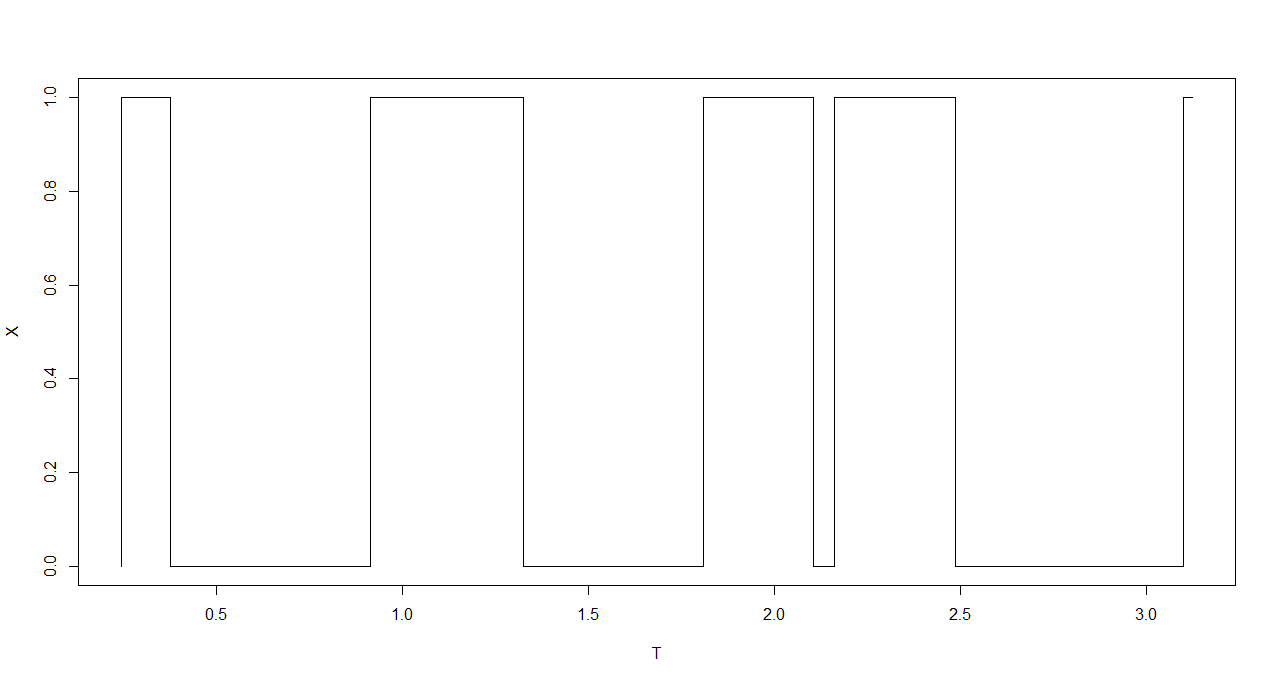
\includegraphics[width=0.7\textwidth]{cadenamarkovtc.png}
\caption{Simulaci\'on de Cadena de Markov con matriz infinitesimal Q}
\label{3}
\end{figure}
\item Utilice su programa para generar 10000 trayectorias en el intervalo de tiempo $[0,10]$ comenzando con probabilidad $1/2$ en cada estado y obtenga la distribuci\'on emp\'irica de $X_{10}$.
\begin{lstlisting}
cont=0
for(j in 1:10000){
X=0
p=.5
if(runif(1)<p){
X=0
T=rexp(1,2)
}else{
X=1
T=rexp(1,3)
}
i=2
while(T[i-1]<=10){
if(X[i-1]==0){
X[i]=1
T[i]=T[i-1]+rexp(1,3)
}else{
X[i]=0
T[i]=T[i-1]+rexp(1,2)
}
i=i+1
}
if(X[i-1]==0){
cont=cont+1
}
}

p0=cont/10000
p1=1-p0
p0
p1

Distribuci\'on emp\'irica
> p0
[1] 0.6084
> p1
[1] 0.3916
\end{lstlisting} 
\item Calcule $e^{10Q}$ (utilizando alg\'un comando adecuado) y contraste con la distribuci\'on emp\'irica del inciso anterior.
\begin{lstlisting}
library(Matrix)
Q= cbind(c(-2,3),c(2,-3))
P_10=expm(10*Q)
P_10

> P_10
2 x 2 Matrix of class "dgeMatrix"
     [,1] [,2]
[1,]  0.6  0.4
[2,]  0.6  0.4
\end{lstlisting}
\item Codifique el siguiente esquema num\'erico, conocido como m\'etodo de Euler, para aproximar a $e^{10 Q}$: escoja $h>0$ peque\~no, defina a $P^h_0$ como la matriz identidad y recursivamente\begin{esn}
P^h_{i+1}=P^h_i+hQP^h_i. 
\end{esn}corra hasta que $i=\floor{10/h}$ y compare la matriz resultante con $e^{10Q}$. Si no se parecen escoja a $h$ m\'as peque\~no. ?`Con qu\'e $h$ puede aproximar a $e^{10Q}$ a 6 decimales?
\begin{lstlisting}
options(digits=6)
Q= cbind(c(-2,3),c(2,-3))
h=.3
P=diag(1,2)
k=floor(10/h)
for(i in 1:k){
P=P+h*(Q%*%P)
}
P
> P
     [,1] [,2]
[1,]  0.6  0.4
[2,]  0.6  0.4

Por lo tanto con h=.3 se puede aproximar a P con 6 decimales.
\end{lstlisting}
\end{enumerate}
\end{problema}


\begin{problema}
Un proceso estoc\'astico $B=\paren{B_t,t\geq 0}$ es un movimiento browniano en ley si y s\'olo si es un proceso gaussiano centrado y $\esp{B_sB_t}=s\wedge t$. 
\begin{proof}
Supongamos que $B=\paren{B_t,t\geq 0}$ es un movimiento browniano en ley. Tenemos que demostrar que $(B_{t_1},B_{t_2},...,B_{t_n})$ en vector gausssino con $(t_1<t_2...<t_n)$, como $B$ es un movimiento Browniano sabemos que $(B_{t_1},B_{t_2}-B_{t_1},...,B_{t_n}-B_{t_{n-1}})$ es un vector gaussiano ya que son variables aleatorias normales independientes y cualquier combinaci\'on lineal de normales independientes es normal. Entonces cualquier combinaci\'on lineal la podemes escribir:
\begin{esn}
\sum_{i=1}^n \lambda_i B_{t_i}=\sum_{i=1}^{n} \alpha_i (B_{t_{i}}-B_{t_{i-1}})
\end{esn}

donde $(B_{t_0})=0$.

Por lo tanto $\sum_{i=1}^n \lambda_i B_{t_i}$ se distribuye normal y $\esp{B_{t_i}}=0$.

Por lo tanto $B$ es un proceso gaussiano centrado.

Y ademas como es un movimiento browniano sabemos que $\esp{B_sB_t}=s\wedge t$ por ser movimiento Browniano.

Ahora supongamos que es un proceso gaussiano centrado y $\esp{B_sB_t}=s\wedge t$. Luego entonces como $\esp{B_0}=0$ y ya que $\esp{B_sB_t}=s\wedge t$ entonces $\var{B_0}=\esp{B_0B_0}=0$. Por lo tanto $B_0=0$.
Por el mismo argumento que en la necesidad cualquier combinaci\'on lineal la podemos escrbir de la siguiente manera:

\begin{esn}
\sum_{i=1}^n \lambda_i B_{t_i}=\sum_{i=1}^{n} \alpha_i (B_{t_{i}}-B_{t_{i-1}}).
\end{esn}

Por lo tanto los incrementos del proceso gaussiano centrado tambien forman un proceso gaussiano.


Ahora para ver que tiene incrementos independientes como estamos en un proceso gaussiano solo nos basta verificar que la correlacion es cero. Sea $t_i<t_j$:

\begin{align}
\esp{(B_{t_i}-B_{t_{i-1}})(B_{t_j}-B_{t_{j-1}})}&=\esp{B_{t_{i}}B_{t_{j}}-B_{t_{i}}B_{t_{j-1}}-B_{t_{i-1}}B_{t_{j}}+B_{t_{i-1}}B_{t_{j-1}}}\notag \\
&=\esp{B_{t_{i}}B_{t_{j}}}-\esp{B_{t_{i}}B_{t_{j-1}}}-\esp{B_{t_{i-1}}B_{t_{j}}}+\esp{B_{t_{i-1}}B_{t_{j-1}}}\notag \\
&=t_i-t_i-t_{i-1}+t_{i-1}\notag \\
&=0.\notag
\end{align}

Por lo tanto $B$ tiene incrementos independientes.

Ahora veamos que $B$ tiene incrementos estacionarios, es decir $B_{t+s}-B_t=B_s$ en distribuci\'on. como $B_{t+s}-B_t$ es una combinaci\'on lineal del proceso gaussianos entonces sabemos que es normal. Adem\'as como es un proceso gaussiano sabemos que $\esp{B_{t+s}-B_t}=0$. Ahora calculemos la varianza:

\begin{align}
\var{B_{t+s}-B_t}&=\esp{(B_{t+s}-B_t)^2}\notag \\
&=\esp{B_{t+s}B_{t+s}}-\esp{B_{t+s}B_{t}}-\esp{B_{t}B_{t+s}}+\esp{B_{t}B_{t}}\notag \\
&=t+s-t-t+t\notag \\
&=s\notag
\end{align}

Por lo tanto $B_{t+s}-B_t$ se distribuye $N(0,s)$.

Por lo tanto $B_{t+s}-B_t=B_s$ en distribuci\'on.

Para concluir como $B$ es un proceso gaussiano centrado y ademas la $\var{B_t}=\esp{B_tB_t}=t$.
Por lo tanto $B_t$ se distribuye $N(0,t)$.

Por lo tanto $B$ es un movimiento browniano en ley.
\end{proof}
\end{problema}
\begin{problema}
El objetivo de este problema es construir, a partir de movimientos brownianos en $[0,1]$, al movimiento browniano en $[0,\infty)$.
\begin{enumerate}
\item Pruebe que existe un espacio de probabilidad $\ofp$ en el que existe una sucesi\'on $B^1,B^2,\ldots$ de movimientos brownianos en $[0,1]$ independientes. (Sugerencia: utilice la construcci\'on del movimiento browniano de L\'evy  para que la soluci\'on sea corta.)
\item Defina a $B_t=B^1_1+\cdots+B^{\floor{t}}_1+B^{\ceil{t}}_{t-\floor{t}}$ para $t\geq 0$. Pruebe que $B$ es un movimiento browniano. 

\begin{proof}
Primero notemos que $B_0=0$ ya que $B_0=B_{0}^1=0$.

Utilizaremos el ejercicio anterior para ver que es un movimento browniano. Primero demostraremos que $B_t$ es un proceso gaussiano:

Falta

Ahora veamos que es un proceso gaussiano centrado:

\begin{align}
\esp{B_t}&=\esp{B^1_1+\cdots+B^{\floor{t}}_1+B^{\ceil{t}}_{t-\floor{t}}}\notag \\
&=\esp{B^1_1}+\cdots+\esp{B^{\floor{t}}_1}+\esp{B^{\ceil{t}}_{t-\floor{t}}} \notag \\
&=0.
\end{align}

Calculemos la varianza:

\begin{align}
\var{B_t}&=\var{B^1_1+\cdots+B^{\floor{t}}_1+B^{\ceil{t}}_{t-\floor{t}}}\notag \\
&=\var{B^1_1}+\cdots+\var{B^{\floor{t}}_1}+\var{B^{\ceil{t}}_{t-\floor{t}}} \notag \\
&=\floor{t}+t-\floor{t}\notag \\
&=t\notag
\end{align}

Por lo tanto $B_t$ se distribuye $N(0,t)$.

Ahora verificaremos que $\esp{B_sB_t}=s\wedge t$:

Si $s=t$ tenemos que $\esp{B_tB_s}=\esp{B_t^2}=t=t\wedge s$.
Supongamos que $t<s$:

Supongamos primero que $\floor{t}\leq t<s\leq\ceil{t}$. Entonces:
\begin{align}
B_t&=B^1_1+\cdots+B^{\floor{t}}_1+B^{\ceil{t}}_{t-\floor{t}}\notag \\
B_s&=B^1_1+\cdots+B^{\floor{t}}_1+B^{\ceil{t}}_{s-\floor{t}}\notag
\end{align}

Utilizando el hecho de que $B^n$ son independientes obtenemos que:
\begin{align}
\esp{B_tB_s}&=\esp{(B^1_1)^2}+...+\esp{(B^{\floor{t}}_1)^2}+\esp{B^{\ceil{t}}_{t-\floor{t}}B^{\ceil{t}}_{s-\floor{t}}}\notag \\
&=\floor{t}+\esp{B^{\ceil{t}}_{t-\floor{t}}B^{\ceil{t}}_{s-\floor{t}}} \notag \\
&=\floor{t}+(t-\floor{t})\wedge(s-\floor{t}\notag \\
&=\floor{t}+t-\floor{t} \notag \\
&=t\notag
\end{align}

Ahora supongamos que $\floor{t}\leq t\leq\ceil{t}< s$. Entonces:

\begin{align}
B_t&=B^1_1+...+B^{\floor{t}}_1+B^{\ceil{t}}_{t-\floor{t}}\notag
B_s&=B^1_1+...+B^{\floor{t}}_1+B^{\ceil{t}}_1+B^{\ceil{t}+1}_1+...+B^{\floor{s}}_1+B^{\ceil{s}}_{s-\floor{s}}\notag \\
\end{align}

Como $B^n$ son independientes tenemos que:
\begin{align}
\esp{B_tB_s}&=\esp{(B^1_1)^2}+...+\esp{(B^{\floor{t}}_1)^2}+\esp{B^{\ceil{t}}_{t-\floor{t}}B^{\ceil{t}}_{1} }\notag \\
&=\sum_{i=1}^{\floor{t}}\esp{(B^i_1)^2}+t-\floor{t}\notag \\
&=\floor{t}+t-\floor{t}\notag
=t\notag
\end{align}

Por lo tanto $\esp{B_tB_s}=s\wedge t$.

Por lo tanto por el ejercicio anterior obtenemos que $B_t$ es un movimiento browniano en ley.

Y ademas como cada $B^n$ es continua y adem\'as $B_0^n=$ para toda $n\in\na$ entonces $B_t$ es continua.

\end{proof}
%\item Pruebe que $\paren{B_t}^2-t$ no tiene incrementos independientes. Sugerencia: En el ejercicio anterior identific\'o la distribuci\'on de $\paren{B_t}^2$; calcule la transformada de Laplace conjunta de dos incrementos.
\end{enumerate}
\end{problema}
\begin{problema}
Pruebe que si $\tilde X$ es una modificaci\'on de $X$ entonces ambos procesos tienen las mismas distribuciones finito-dimensionales. Concluya que si
 $B$ es un movimiento browniano en ley y $\tilde B$ es una modificaci\'on de $B$ con trayectorias continuas entonces $\tilde B$ es un movimiento browniano.

\begin{proof}

Sea $0\leq t_1<t_2<t_3...<t_n$. Primeros veamos que $A_n=\{X_{t_1}=\hat{X_{t_1}},X_{t_2}=\hat{X_{t_2}},...,X_{t_n}=\hat{X_{t_n}}\}$ tiene probabilidad 1. Lo haremos por inducci\'on.

Por definición de modificacion de $X$ sabemos que $\proba{A_1}=1$.

Supongamos caso $n=k$, es decir que $\proba{A_k}=1$.

Demostraremos caso $n=k+1$:

\begin{align}
\proba{A_{k+1}}&=\proba{A_k\cap \{X_{_{k+1}}=\hat{X_{t_{k+1}}}\}}\notag
\intertext{Como los dos eventos tienen probabilidad 1 entonces:}
\proba{A_{k+1}}&=1.\notag
\end{align}

Por lo tanto $\proba{A_n}=1$.

Ahora demostraremos la proposici\'on:

\begin{align}
&\proba{X_{t_1}\leq x_1,..., X_{t_n}\leq x_n}=\proba{X_{t_1}\leq x_1,..., X_{t_n}\leq x_n,A_n\cup A_n^c}\notag \\
&=\proba{X_{t_1}\leq x_1,..., X_{t_n}\leq x_n,A_n}+\proba{X_{t_1}\leq x_1,..., X_{t_n}\leq x_n, A_n^c} \notag
\intertext{Como $\proba{A_n}=1$ entonces $\proba{A_n^c}=0$, entonces:}
&=\proba{\proba{X_{t_1}\leq x_1,..., X_{t_n}\leq x_n,A_n}} \notag \\
&=\probac{X_{t_1}\leq x_1,..., X_{t_n}\leq x_n}{A_n}\proba{A_n}\notag \\
&=\probac{X_{t_1}\leq x_1,..., X_{t_n}\leq x_n}{A_n} \notag \\
&=\probac{\hat{X_{t_1}}\leq x_1,...,\hat{X_{t_n}}\leq x_n}{A_n} \notag \\
&=\frac{\proba{\hat{X_{t_1}}\leq x_1,...,\hat{X_{t_n}}\leq x_n,A_n}}{\proba{A_n}}\notag \\
&=\proba{\hat{X_{t_1}}\leq x_1,...,\hat{X_{t_n}}\leq x_n,A_n} \notag \\
&=\proba{\hat{X_{t_1}}\leq x_1,...,\hat{X_{t_n}}\leq x_n,A_n}+\proba{\hat{X_{t_1}}\leq x_1,...,\hat{X_{t_n}}\leq x_n,A_n^c}\notag \\
&=\proba{\hat{X_{t_1}}\leq x_1,...,\hat{X_{t_n}}\leq x_n,A_n\cup A_n^c}\notag \\
&=\proba{\hat{X_{t_1}}\leq x_1,...,\hat{X_{t_n}}\leq x_n}.\notag
\end{align}

Por lo tanto ambos procesos tienen las mismas distribuciones finito-dimensionales.

Para demostrar que $\tilde{B}$ es un movimiento browniano sabemos que $B$ es un movimiento browniano entonces B es  un proceso gaussiano centrado tal que  $\esp{B_sB_t}=s \wedge t$. Por lo que acabamos de demostrar tenemos que $\tilde{B}$ es un proceso gaussiano centrado tal que $\esp{\tilde{B_s}\tilde{B_t}}=s \wedge t$. Por lo tanto $\tilde{B}$ es un movimiento browniano en ley con trayectorias continuas. Por lo tanto $\tilde{B}$ es un movimiento browniano.

\end{proof}
\end{problema}
\begin{problema}
Sea\begin{esn}
M^\lambda_t=e^{\lambda B_t-\lambda^2t/2}.
\end{esn}
\begin{enumerate}
\item Explique y pruebe formalmente por qu\'e, para toda $n\geq 1$, $\partial^n M^\lambda_t/\partial \lambda^n$ es una martingala.
\begin{proof}
Observemos que $M^\lambda_t$ es martingala.
\begin{itemize}
\item Ya que suponemos que estamos en la filtraci\'on can\'onica entonces $M^\lambda_t$ es adaptado
\item Como $M^\lambda_t=e^{\lambda B_t-\lambda^2t/2} \leq e^{\lambda B_t}$, entonces:
\begin{esn}
\esp{M^\lambda_t}\leq \esp{e^{\lambda B_t}}=e^{\frac{t\lambda^2}{2}}.
\end{esn}
Por lo tanto $M^\lambda_t$ es integrable.
\item  Propiedad de juego justo. Sea $s \leq t$:
\begin{align}
\espc{M^\lambda_t}{\F_s}&=\espc{e^{\lambda B_t-\lambda^2t/2}}{\F_s}\notag  \\ &=e^{-\lambda^2t/2}\espc{e^{\lambda B_t}}{\F_s} \notag \\
&=e^{-\lambda^2t/2}\espc{e^{\lambda( B_t- B_s+B_s) }}{\F_s}\notag \\
&=e^{-\lambda^2t/2+\lambda B_s}\esp{e^{\lambda( B_{t-s}) }}\notag \\
&==e^{-\lambda^2t/2+\lambda B_s}e^{(t-s)\lambda^2/2}\notag \\
&=e^{\lambda B_s-s\lambda^2/2}\notag \\
&=M^\lambda_s \notag
\end{align}

\end{itemize}

Por lo tanto $M^\lambda_t$ es martingala.

Ahora veamos que $\partial^n M^\lambda_t/\partial \lambda^n$ es martingala, para esto utulizaremos el resultado que nos permite intercambiar la esperanza condicional con la derivada, el cual fue demostrado anterioremente. Utilizando inducci\'on:

Caso n=1:

\begin{itemize}
\item $\partial M^\lambda_t/\partial \lambda$ es $\F_t$-medible ya que es limite de funciones $\F_t$- medibles.
\item Verifiquemos que $\partial M^\lambda_t/\partial \lambda$ es integrable:
\begin{align}
\abs{\partial M^\lambda_t/\partial \lambda}&=e^{\lambda B_t-\lambda^2t/2}\abs{(B_t-\lambda t)}\notag \\ &\leq e^{\lambda B_t-\lambda^2t/2}\abs{B_t}+e^{\lambda B_t-\lambda^2t/2}\abs{\lambda t}\notag \\
&\leq e^{\lambda B_t} \abs{B_t}+e^{\lambda B_t} \abs{\lambda t}\notag
\intertext{Luego entonces:}
\esp{abs{\partial M^\lambda_t/\partial \lambda}}& \leq \esp{e^{\lambda B_t} \abs{B_t}}+\esp{e^{\lambda B_t} \abs{\lambda t}}\notag \\
&=\int_{-\infty}^{\infty}\abs{u}e^{\lambda u} \frac{1}{\sqrt{2\pi t}}e^{-\frac{u^2}{2t}}du+\abs{\lambda t}e^{t\lambda^2/2}\notag \\
&=e^{t\lambda^2/2}\int_{-\infty}^{\infty}\abs{u}\frac{1}{\sqrt{2\pi t}}e^{-\frac{(u-t\lambda)^2}{2t}}du++\abs{\lambda t}e^{t\lambda^2/2}<\infty \notag
\end{align}

Por lo tanto $\partial M^\lambda_t/\partial \lambda$ es integrable.
Ademas tambien concluimos $\partial M^\lambda_t/\partial \lambda$ esta dominada por $ e^{\lambda B_t} \abs{B_t}+e^{\lambda B_t} \abs{\lambda t}$ que pertenece a $L_1$.

\item La propiedad de juego justo.Ya que $\partial M^\lambda_t/\partial \lambda$ esta dominada entonces podemos intercambiar la derivada con la esperanza:

\begin{align}
\espc{\frac{\partial}{\partial \lambda} M^\lambda_t}{\F_s}&=\frac{\partial}{\partial \lambda} \espc{ M^\lambda_t}{\F_s}\notag \\
&=\frac{\partial}{\partial \lambda}M^\lambda_s \notag
\end{align}

Por lo tanto satsiface la propiedad de juego justo.

\end{itemize}

Por lo tanto $\frac{\partial}{\partial \lambda} M^\lambda_t$ es martingala.

Ahora supongamos $\frac{\partial^k}{\partial \lambda^k} M^\lambda_t$ es martingala.

Por demostrar $\frac{\partial^{k+1}}{\partial \lambda^{k+1}} M^\lambda_t$ es martingala.

\begin{itemize}


\item Supongamos que $\frac{\partial^n}{\partial \lambda^n} M^\lambda_t$ es martingala, por demostrar que  . Dada la hipotesis de inducci\'on tenemos entonces que:
$$
\espc{\frac{\partial^{n+1}}{\partial \lambda^{n+1}} M^\lambda_t}{\F_s}=\espc{\frac{\partial}{\partial \lambda}  \frac{\partial^n}{\partial \lambda^n} M^\lambda_t}{\F_s}=^*\frac{\partial}{\partial \lambda} \espc{ \frac{\partial^n}{\partial \lambda^n} M^\lambda_t}{\F_s}
$$
$$
\frac{\partial}{\partial \lambda} \frac{\partial^n}{\partial \lambda^n} M^\lambda_s=\frac{\partial^{n+1}}{\partial \lambda^{n+1}}M^\lambda_s
$$
Lo que demostrar\'ia  que $\frac{\partial^{n+1}}{\partial \lambda^{n+1}} M^\lambda_t$ tiene la propiedad de martingala\\
(*) Faltaria probar que  $\frac{\partial^n}{\partial \lambda^n} M^\lambda_t $ es dominada por una funci\'on integrable para poder sacar el operador derivada de la esperanza condicional
\end{itemize}
\end{proof}
\item Sea $\imf{H_n}{x}=\paren{-1}^ne^{x^2/2}\frac{d^n}{dx^n}e^{-x^2/2}$. A $H_n$ se le conoce como en\'esimo polinomio de Hermite. Calc\'ulelo para $n\leq 5$. Pruebe que $H_n$ es un polinomio para toda $n\in\na$ y que $\partial^n M^\lambda_t/\partial \lambda^n=t^{n/2}\imf{H_n}{B_t/\sqrt{t}}M^\lambda_t$. 
\item Pruebe que $t^{n/2}\imf{H_n}{B_t/\sqrt{t}}$ es una martingala para toda $n$ y calc\'ulela para $n\leq 5$. 
\item Aplique muestreo opcional a las martingalas anteriores al tiempo aleatorio $T_{a,b}=\min\set{t\geq 0:B_t\in\set{-a,b}}$ (para $a,b>0$) con $n=1,2$ para calcular $\proba{B_{T_{a,b}}=b}$ y $\esp{T_{a,b}}$, �Qu\'e concluye cuando $n=3,4$? ?` Cree que $T_{a,b}$ tenga momentos finitos de cualquier orden? Justifique su respuesta.
\item Aplique el teorema de muestreo opcional a la martingala $M^\lambda $ al tiempo aleatorio $T_a=\inf\set{t\geq 0:B_t\geq a}$ si $\lambda>0$. Diga por qu\'e es necesaria la \'ultima hip\'otesis y calcule la transformada de Laplace de $T_a$. 
\item Opcional (para subir calificaci\'on en esta u otra tarea): 
\begin{enumerate}
\item Modifique el ejercicio para que aplique al proceso Poisson.
\item Resu\'elva el ejercicio modificado. 
\end{enumerate}
\end{enumerate}
\end{problema}
\begin{problema}\mbox{}
\begin{enumerate}
\item Al aplicar la desigualdad maximal de Doob sobre los racionales de orden $n$ y pasar al l\'imite conforme $n\to\infty$, pruebe que $\sup_{t\leq }\abs{B_t-B_1}$ es cuadrado integrable.
\item Pruebe que la sucesi\'on de variables aleatorias\begin{esn}
\paren{\sup_{t\in [0,1]}\abs{B_{n+t}-B_n},n\in\na}
\end{esn}son independientes, id\'enticamente distribuidas y de media finita. (Utilice la propiedad de Markov.)
\item Al utilizar Borel-Cantelli, pruebe que, para cualquier $C>0$ fija\begin{esn}
\limsup_{n\to\infty}\sup_{t\in [0,1]}\abs{B_{n+t}-B_n}/n\leq C\end{esn} casi seguramente.
\item Pruebe que $\paren{B_n/n,n\geq 1}$ converge casi seguramente a $0$ y deduzca que\begin{esn}
\lim_{t\to\infty }B_t/t=0.
\end{esn}
\end{enumerate}
\end{problema}
%
%\begin{problema}
%Sean $\F_1,\F_2,\ldots $ y $\G$ sub\sa s de $\F$. Decimos que $\F_1,\F_2,\ldots$ son condicionalmente independientes dada $\G$ si para cualquier $H_i$ que sea $\F_i$ medible y acotada se tiene que\begin{esn}
%\espc{H_1\cdots H_n}{\G}=\espc{H_1}{\G}\cdots \espc{H_n}{\G}.
%\end{esn}
%\begin{enumerate}
%\item ?`Qu\'e quiere decir la independencia condicional cuando $\G=\set{\oo,\emptyset}$?
%\item Pruebe que $F_1$ y $\F_2$ son condicionalmente independientes dada $\G$ (denotado $\condind{\F_1}{\F_2}{\G}$) si y s\'olo si para cualquier $H$ que sea $\F_1$-medible y acotada se tiene que\begin{esn}
%\espc{H}{\F_2,\G}=\espc{H}{\G}.
%\end{esn}
%\item Pruebe que $\F_1,\F_2,\ldots, $ son condicionalmente independientes dada $\G$ si y s\'olo si para cada $n\geq 1$, $\F_{n+1}$ es condicionalmente independiente de $\F_1,\ldots, \F_n$ dada $\G$. 
%\end{enumerate}
%
%\defin{Categor\'ias: } Esperanza condicional, Independencia condicional.
%\end{problema}
%
%\begin{problema}
%Sea $\mu$ una distribuci\'on de progenie y defina $\tilde \mu_j=\mu_{j+1}$. Sea $S=\paren{S_n}$ una caminata aleatoria con distribuci\'on de salto $\tilde\mu$. Sea $k$ un entero no-negativo y defina recursivamente\begin{esn}
%Z_0=k=C_0,\quad Z_{n+1}=k+S_{C_n}\quad\text{y} C_{n+1}=C_n+Z_{n+1}.
%\end{esn}
%\begin{enumerate}
%\item Pruebe que $Z_n\geq 0$ para toda $n$ y que si $Z_n=0$ entonces $Z_{n+1}=0$.
%\item Pruebe que $C_n$ es un tiempo de paro para la filtraci\'on can\'onica asociada a $S$.
%\item Pruebe que $Z$ es un proceso de Galton-Watson con ley de progenie $\mu$. 
%\item Pruebe que si $S$ alcanza $-1$ entonces existe $n$ tal que $Z_n=0$. Deduzca que si la media de $\mu$ es $1$ entonces $Z$ se extingue. (Sugerencia: utilice un ejercicio anterior sobre martingalas con saltos acotados hacia abajo.) 
%\end{enumerate}
%
%\defin{Categor\'ias: } Caminatas aleatorias, Procesos de Galton-Watson%, Propiedad de Markov fuerte.
%\end{problema}
%
%\begin{problema}
%Sea $\mu$ una distribuci\'on de progenie y defina $\tilde \mu_j=\mu_{j+1}$. Sea $\nu$ una distribuci\'on en $\na$. Consideremos a dos caminatas aleatorias $S=\paren{S_n}$  y $T$ con  distribuci\'ones de salto $\tilde\mu$ y $\nu$.
%\begin{enumerate}
%\item ?`Qu\'e significa que $S$ y $T$ sean independientes? As\'umalo.
%\item Sea $k$ un entero no-negativo y defina recursivamente\begin{esn}
%Z_0=k=C_0,\quad Z_{n+1}=k+S_{C_n}+T_n\quad\text{y} C_{n+1}=C_n+Z_{n+1}.
%\end{esn}
%\item Pruebe que $Z_n\geq 0$ para toda $n$.
%\item Pruebe que $C_n=k\in\F^S_k\cap\F^T_n$.
%\item Pruebe que $Z$ es un proceso de Galton-Watson con inmigraci\'on.
%\end{enumerate}
%
%\defin{Categor\'ias: } Caminatas aleatorias, Procesos de Galton-Watson, Construcci\'on de procesos estoc\'asticos
%\end{problema}
%
%\begin{problema} %Construcci\'on tipo Poisson 
%Sean $\mu$ y $\nu$ una distribuci\'on de progenie y de inmigraci\'on. Sean $Y_1,Y_2,\ldots$ independientes y de ley $\nu$. Suponga que condicionalmente a $Y$, $X^0,X^1,X^2,\ldots$ son procesos de Galton-Watson independientes tales que $X^0_0=k$ y $X^k_0=Y_k$ para $k\geq 1$. Pruebe que si\begin{esn}
%Z_n=\sum_{k=0}^n X^k_{n-k},
%\end{esn}entonces $Z$ es un proceso de Galton-Watson con distribuciones de progenie e inmigraci\'on $\mu$ y $\nu$ que comienza en $k$. 
%
%\defin{Categor\'ias: } Procesos de ramificaci\'on
%\end{problema}
%
%\begin{problema}
%Para cada par de medidas de probabilidad en $\na^\na$ $\p_1$ y $\p_2$ definimos a la convoluci\'on de $\p_1$ y $\p_2$, denotada $\p_1 *\p_2$, como la distribuci\'on de $\paren{S^1_k+S^2_k,k\geq 0}$ donde $S^1$ y $S^2$ son independientes y de distribuciones $\p_1$ y $\p_2$ respectivamente.
%\begin{enumerate}
%\item ?` Cu\'al es la relaci\'on entre las distribuciones finito-dimensionales de $\p_1$, $\p_2$ y $\p_1*\p_2$?
%\item Sea $\p_k^\mu$ la distribuci\'on de un proceso de Galton-Watson  de ley de reproducci\'on $\mu$ que comienza en $k$. Pruebe que $\p_{k_1}*\p_{k_2}=\p_{k_1+k_2}$.
%%\item Caracterizaci\'on de leyes markovianas con la propiedad de ramificaci\'on.
%\end{enumerate}
%
%\defin{Categor\'ias: } Distribuciones finito-dimensionales, Procesos de ramificaci\'on.
%\end{problema}
\bibliographystyle{amsalpha}

\end{document}